\documentclass[12pt, a4paper]{report}

\usepackage[utf8]{inputenc}
\usepackage[T1]{fontenc}
\usepackage{listings}
\lstdefinelanguage{Solidity}{
  keywords={pragma,solidity,contract,function,returns,external,internal,public,private,
             view,pure,payable,mapping,address,uint256,uint,bool,bytes32,string,
             event,emit,modifier,require,revert,import,is,memory,storage,indexed,
             bytes,keccak256,struct,enum,constructor,fallback,receive},
  sensitive=true,
  comment=[l]{//},
  morecomment=[s]{/*}{*/},
  morestring=[b]",
}
\lstset{
  basicstyle=\ttfamily\scriptsize,
  keywordstyle=\bfseries,
  commentstyle=\color{black!55}\itshape,
  stringstyle=\itshape,
  breaklines=true,
  frame=tb,
  rulecolor=\color{black!55},
  captionpos=b,
  numbers=left,
  numberstyle=\tiny\color{black!55},
  xleftmargin=2em,
}
\IfFileExists{libertine.sty}{%
  \usepackage[mono=false]{libertine}%
  \IfFileExists{zi4.sty}{\usepackage[varqu]{zi4}}{}%
}{%
  \usepackage{lmodern}%
}
\usepackage[protrusion=true, expansion=false]{microtype}
\usepackage[a4paper, width=155mm, top=25mm, bottom=25mm, headheight=15pt]{geometry}
\usepackage{setspace}
\onehalfspacing
\emergencystretch=3em
\hbadness=2000

\usepackage{amsmath,amssymb}
\usepackage{fontawesome5}
\newcommand{\tmarkDone}{\textbf{\faCheck}}
\newcommand{\tmarkNo}{\textbf{\faTimes}}
\newcommand{\tmarkPartial}{\faHourglassHalf}
\newcommand{\tmarkPlanned}{\textcolor{black!55}{\faCircle}}

\usepackage{graphicx}
% Overleaf / self-contained build: all figure assets live in overleaf/ (PNG + vector PDF).
\newcommand*{\ThesisDiagDir}{overleaf/}
\graphicspath{{overleaf/}{./}}
\pdfimageresolution=300
\makeatletter
\newcommand*{\@thesis@doinclude}[2]{%
  \if\relax\detokenize{#1}\relax
    \includegraphics{#2}%
  \else
    \includegraphics[#1]{#2}%
  \fi
}
\newcommand*{\@thesismissingimg}[1]{%
  \fbox{\parbox{0.92\linewidth}{\scriptsize\centering\ttfamily Missing file: \detokenize{#1}.\\[2pt]Add it to the \texttt{overleaf/} folder and recompile.}}%
}
\newcommand{\ThesisIncludeGraphics}[2][]{%
  \IfFileExists{\ThesisDiagDir#2}{%
    \@thesis@doinclude{#1}{\ThesisDiagDir#2}}{%
  \IfFileExists{#2}{%
    \@thesis@doinclude{#1}{#2}}{%
    \@thesismissingimg{#2}%
  }}%
}
\makeatother
\newcommand{\TableScreenshotEnd}[2][]{%
  \refstepcounter{table}%
  \if\relax\detokenize{#1}\relax\else\label{#1}\fi%
  \phantomsection%
  \addcontentsline{lot}{table}{\protect\numberline{\thetable}#2}%
}
\usepackage[table]{xcolor}
\usepackage{tikz}
\usetikzlibrary{arrows.meta,positioning,fit,shapes.geometric,calc}
\usepackage{pgfplots}
\usepgfplotslibrary{statistics}
\pgfplotsset{compat=1.18, minor tick num=0}

\usepackage{booktabs}
\usepackage{array}
\usepackage{colortbl}
\usepackage{multirow}
\usepackage{float}
\usepackage{etoolbox}
\usepackage{caption}
\captionsetup{
    labelfont={bf,small},
    textfont={small},
    skip=6pt,
    format=hang
}
\makeatletter
% Compact, professional List of Figures / List of Tables (no tocloft dependency)
\renewcommand*\l@figure{\@dottedtocline{1}{0em}{3.2em}}
\renewcommand*\l@table{\@dottedtocline{1}{0em}{3.8em}}
\makeatother

\newlength{\ThesisTableImgReserve}
\newlength{\ThesisFigImgReserve}
\setlength{\ThesisTableImgReserve}{\dimexpr2\intextsep+0.75\baselineskip\relax}
\setlength{\ThesisFigImgReserve}{\dimexpr2\intextsep+\abovecaptionskip+\belowcaptionskip+4\baselineskip\relax}
\newcommand{\TableImageMaxFit}[1]{%
  \ThesisIncludeGraphics[
    width=0.7\linewidth,
    height=\dimexpr(\textheight-\ThesisTableImgReserve)*7/10\relax,
    keepaspectratio
  ]{#1}%
}
\newcommand{\FigureImageMaxFit}[1]{%
  \ThesisIncludeGraphics[width=\linewidth,height=\dimexpr\textheight-\ThesisFigImgReserve\relax,keepaspectratio]{#1}%
}
\newcommand{\OnePageDiagram}[2][]{%
  \if\relax\detokenize{#1}\relax
    \ThesisIncludeGraphics[width=\linewidth,height=\dimexpr\textheight-\ThesisFigImgReserve\relax,keepaspectratio]{#2}%
  \else
    \ThesisIncludeGraphics[#1,width=\linewidth,height=\dimexpr\textheight-\ThesisFigImgReserve\relax,keepaspectratio]{#2}%
  \fi
}
\newcommand{\HalfWidthDiagram}[1]{%
  \ThesisIncludeGraphics[width=0.5\linewidth, keepaspectratio]{#1}%
}
\newcommand{\WideDiagram}[2][]{%
  \if\relax\detokenize{#1}\relax
    \ThesisIncludeGraphics[width=\linewidth, height=0.78\textheight, keepaspectratio]{#2}%
  \else
    \ThesisIncludeGraphics[#1, width=\linewidth, height=0.78\textheight, keepaspectratio]{#2}%
  \fi
}
\newcommand{\TallDiagram}[2][]{%
  \if\relax\detokenize{#1}\relax
    \ThesisIncludeGraphics[width=\linewidth, height=0.96\textheight, keepaspectratio]{#2}%
  \else
    \ThesisIncludeGraphics[#1, width=\linewidth, height=0.96\textheight, keepaspectratio]{#2}%
  \fi
}
% Balanced layout slot (reference: Figure 4.3 ml-explainability) — wide banded diagrams.
\newcommand{\BalancedDiagram}[2][]{%
  \if\relax\detokenize{#1}\relax
    \ThesisIncludeGraphics[width=\linewidth, height=0.72\textheight, keepaspectratio]{#2}%
  \else
    \ThesisIncludeGraphics[#1, width=\linewidth, height=0.72\textheight, keepaspectratio]{#2}%
  \fi
}
% Activity diagrams — full-height slot for 3× label size.
\newcommand{\ActivityDiagram}[2][]{%
  \if\relax\detokenize{#1}\relax
    \ThesisIncludeGraphics[width=\linewidth, height=\textheight, keepaspectratio]{#2}%
  \else
    \ThesisIncludeGraphics[#1, width=\linewidth, height=\textheight, keepaspectratio]{#2}%
  \fi
}
% Half-size slot (50\% of BalancedDiagram width and height).
\newcommand{\CompactDiagram}[2][]{%
  \if\relax\detokenize{#1}\relax
    \ThesisIncludeGraphics[width=0.5\linewidth, height=0.36\textheight, keepaspectratio]{#2}%
  \else
    \ThesisIncludeGraphics[#1, width=0.5\linewidth, height=0.36\textheight, keepaspectratio]{#2}%
  \fi
}

\usepackage[skins]{tcolorbox}

\usepackage{titlesec}
\usepackage{parskip}
\usepackage{fancyhdr}
\usepackage{enumitem}
\PassOptionsToPackage{hyphens,spaces,obeyspaces}{url}
\usepackage{hyperref}
\makeatletter
\g@addto@macro\UrlBreaks{\do\/\do\-\do\.\do\:\do\&\do\=\do\#}
\makeatother

\definecolor{PrimaryBlue}{HTML}{000000}
\definecolor{AccentBlue}{gray}{0.55}
\definecolor{LightBlue}{gray}{0.96}
\definecolor{MidBlue}{gray}{0.90}
\definecolor{DarkText}{HTML}{000000}
\definecolor{GrayText}{gray}{0.45}
\definecolor{RowShade}{gray}{0.965}
\definecolor{RowShadeAlt}{gray}{0.92}
\definecolor{TableHeadBg}{gray}{0.88}
\definecolor{TableRule}{gray}{0.55}
\definecolor{GreenAccent}{HTML}{000000}
\definecolor{AmberAccent}{HTML}{000000}
\definecolor{RedAccent}{HTML}{000000}
\definecolor{VioletAccent}{HTML}{000000}

\hypersetup{
    colorlinks=true,
    linkcolor=black,
    filecolor=black,
    urlcolor=black,
    citecolor=black,
    pdfborder={0 0 0},
}

\titleformat{\chapter}[display]
    {\normalfont\LARGE\bfseries}
    {\chaptertitlename\ \thechapter}{20pt}{\LARGE}
    [\vspace{4pt}{\color{black!40}\titlerule[0.6pt]}]

\titleformat{\section}
    {\large\bfseries}
    {\thesection}{0.8em}{}

\titleformat{\subsection}
    {\normalsize\bfseries}
    {\thesubsection}{0.6em}{}

\titleformat{\subsubsection}
    {\normalsize\bfseries\itshape}
    {\thesubsubsection}{0.6em}{}

\titlespacing*{\chapter}{0pt}{-20pt}{20pt}
\titlespacing*{\section}{0pt}{16pt plus 3pt minus 2pt}{8pt plus 2pt minus 1pt}
\titlespacing*{\subsection}{0pt}{12pt plus 2pt minus 1pt}{6pt plus 1pt minus 1pt}
\titlespacing*{\subsubsection}{0pt}{10pt plus 2pt minus 1pt}{4pt plus 1pt minus 1pt}

\newcommand{\tableheadcolor}{\rowcolor{TableHeadBg}}
\newcommand{\tableheadfont}{\bfseries}
\newcommand{\ThesisTableBodyFont}{\small}

% Consistent greyscale table polish (font size unchanged; spacing only).
\newcommand{\ThesisTablePrep}{%
  \ThesisTableBodyFont
  \renewcommand{\arraystretch}{1.22}%
  \setlength{\tabcolsep}{6pt}%
  \arrayrulecolor{TableRule}%
  \setlength{\aboverulesep}{0.55ex}%
  \setlength{\belowrulesep}{0.55ex}%
}
\AtBeginEnvironment{table}{\ThesisTablePrep}
\AtBeginEnvironment{tabular}{%
  \rowcolors{2}{}{RowShade}%
  \arrayrulecolor{TableRule}%
}

\newenvironment{moderntable}[1][H]{%
    \begin{table}[#1]\centering\ThesisTablePrep
}{%
    \end{table}%
}

\newtcolorbox{layerbox}[1]{
    colback=white,
    colframe=black!55,
    coltitle=black,
    fonttitle=\bfseries\small,
    title=#1,
    boxrule=0.6pt,
    arc=2pt,
    left=6pt,right=6pt,top=4pt,bottom=4pt,
}

\newtcolorbox{highlightbox}[1][]{
    colback=black!4,
    colframe=black!45,
    boxrule=0.5pt,
    arc=2pt,
    left=8pt,right=8pt,top=6pt,bottom=6pt,
    #1
}

\pagestyle{fancy}
\fancyhf{}
\renewcommand{\headrulewidth}{0.4pt}
\fancyhead[L]{\small\color{black!55}Crypto World Bank}
\fancyhead[R]{\small\color{black!55}BRAC University}
\fancyfoot[C]{\small\color{black!55}\thepage}

\newcommand{\manualpie}[6]{%
  \fill[#6] (#1,#2) -- ++({#4}:{#3}) arc ({#4}:{#5}:{#3}) -- cycle;
  \draw[white, line width=0.8pt] (#1,#2) -- ++({#4}:{#3}) arc ({#4}:{#5}:{#3}) -- cycle;
}
\newcommand{\ddcat}[3]{\node[draw=black!55, fill=black!5, rounded corners=2pt, minimum width=2.2cm, minimum height=0.65cm, align=center, font=\scriptsize]
  (#1) at (#2) {#3};}
\newcommand{\ddone}[3]{\node[draw=black, fill=black!22, minimum width=2.2cm, minimum height=0.65cm, align=center, font=\scriptsize\bfseries, rounded corners=2pt] (#1) at #2 {#3};}
\newcommand{\ddtwo}[3]{\node[draw=black!55, fill=white, minimum width=2.2cm, minimum height=0.65cm, align=center, font=\scriptsize, rounded corners=2pt] (#1) at #2 {#3};}

\begin{document}

%% ============================================================
%% TITLE PAGE
%% ============================================================
\thispagestyle{empty}

\begin{center}

\vspace*{0.3cm}

\ThesisIncludeGraphics[width=3.5cm]{bracu_logo_12-0-2022.png}

\vspace{0.8cm}

{\LARGE\bfseries\color{PrimaryBlue} Decentralized Crypto World Bank}\\[0.4em]
{\large\color{PrimaryBlue!80} A Blockchain-Based Lending Platform\\[0.15em]with AI-Enhanced Security}

\vspace{0.6cm}

{\normalsize\bfseries Thesis ID: [P26101123]}

\vspace{1.2cm}

{\large by}

\vspace{0.5cm}

{\Large\bfseries\color{PrimaryBlue} Md.\ Bokhtiar Rahman Juboraz}\\[0.2em]
{\color{GrayText}20301138}\\[0.8em]
{\Large\bfseries\color{PrimaryBlue} Md.\ Mahir Ahnaf Ahmed}\\[0.2em]
{\color{GrayText}20301083}

\vspace{1.2cm}

A pre-thesis 1 report submitted to the Department of Computer Science and Engineering\\
in partial fulfillment of the requirements for the degree of\\
\textbf{B.Sc.\ in Computer Science}

\vfill

{\color{PrimaryBlue}\rule{0.4\textwidth}{0.6pt}}\\[0.6em]
Department of Computer Science and Engineering\\
\textbf{BRAC University}\\
February 2026

\vspace{0.5cm}

{\small\color{GrayText}\copyright\ 2026.\ BRAC University --- All rights reserved.}

\end{center}

%% ============================================================
%% DECLARATION
%% ============================================================
\newpage
\thispagestyle{empty}

\chapter*{Declaration}
\phantomsection
\addcontentsline{toc}{chapter}{Declaration}

It is hereby declared that

\begin{enumerate}
\item The report submitted is our own original work while completing degree at BRAC University.

\item The report does not contain material previously published or written by a third party, except where this is appropriately cited through full and accurate referencing.

\item The report does not contain material which has been accepted, or submitted, for any other degree or diploma at a university or other institution.

\item We have acknowledged all main sources of help.
\end{enumerate}

\vspace{2cm}

\textbf{Student's Full Name \& Signature:}

\vspace{2cm}

\begin{tabular}{p{6cm}p{1cm}p{6cm}}
\hrulefill & & \hrulefill \\
\centering Md. Bokhtiar Rahman Juboraz & & \centering Md. Mahir Ahnaf Ahmed \tabularnewline
\centering 20301138 & & \centering 20301083 \tabularnewline
\end{tabular}

%% ============================================================
%% APPROVAL
%% ============================================================
\newpage
\thispagestyle{empty}

\chapter*{Approval}
\phantomsection
\addcontentsline{toc}{chapter}{Approval}

The pre-thesis 1 report of final year project titled ``Decentralized Crypto World Bank: A Blockchain-Based Lending Platform with AI-Enhanced Security'' submitted by

\begin{enumerate}
\item Md. Bokhtiar Rahman Juboraz (20301138)
\item Md. Mahir Ahnaf Ahmed (20301083)
\end{enumerate}

Of Spring, 2026 has been accepted as satisfactory in partial fulfillment of the requirement for the degree of B.Sc. in Computer Science on February 20, 2026.

\vspace{1cm}

\textbf{Examining Committee:}

\vspace{1.5cm}

\begin{flushleft}
Supervisor:\\
(Member)
\end{flushleft}

\begin{flushright}
\vspace{-0.5cm}
\hrulefill\\
Mr. Annajiat Alim Rasel\\
Senior Lecturer\\
Department of Computer Science and Engineering\\
BRAC University
\end{flushright}

\vspace{1.5cm}

\begin{flushleft}
Project Coordinator:\\
(Member)
\end{flushleft}

\begin{flushright}
\vspace{-0.5cm}
\hrulefill\\
Dr. Md. Golam Rabiul Alam\\
Professor\\
Department of Computer Science and Engineering\\
BRAC University
\end{flushright}

\newpage
\thispagestyle{empty}

\null\vfill

\begin{flushleft}
Head of Department:\\
(Chair)
\end{flushleft}

\begin{flushright}
\vspace{-0.5cm}
\hrulefill\\
Dr. Sadia Hamid Kazi\\
Chairperson and Associate Professor\\
Department of Computer Science and Engineering\\
BRAC University
\end{flushright}

\vfill\null

%% ============================================================
%% ETHICS STATEMENT
%% ============================================================
\newpage
\thispagestyle{empty}

\chapter*{Ethics Statement}
\phantomsection
\addcontentsline{toc}{chapter}{Ethics Statement}

This project operates exclusively on public blockchain test networks using test tokens with no real monetary value. No real financial transactions, personal banking data, or user financial records are involved at any stage of development or evaluation. Artificial Intelligence and Machine Learning (AI/ML) model training and evaluation are \textbf{not executed in pre-thesis 1}; they are planned for the final thesis phase after pre-thesis 2, using synthetically generated or publicly available anonymized datasets. The platform prototype does not process Know Your Customer (KYC) or Anti-Money Laundering (AML) data in its current scope, and all wallet addresses used during testing are disposable testnet addresses. We acknowledge the ethical considerations inherent in AI-assisted financial decision-making and have incorporated explainability mechanisms (SHapley Additive exPlanations, or SHAP) to ensure that automated risk assessments remain transparent and auditable by human reviewers. Future phases plan to incorporate a privacy-preserving ZKP-based identity compliance layer in which users prove KYC status without exposing personal data on-chain; the ethical implications of this design will be evaluated in the final thesis.

%% ============================================================
%% ABSTRACT
%% ============================================================
\newpage
\thispagestyle{empty}

\chapter*{Abstract}
\phantomsection
\addcontentsline{toc}{chapter}{Abstract}

Global development finance relies on multilayered institutional structures to distribute capital across borders and communities, yet these systems often struggle with fragmented transparency, procedural friction, and uneven access to credit. Although decentralized finance has demonstrated that programmable infrastructures can automate lending and enhance auditability, existing models largely employ flat architectures that do not reflect institutional hierarchies or structured governance. As a result, there remains limited exploration of how tiered financial systems might be represented within decentralized environments while preserving oversight and adaptability. Here we present \textit{Crypto World Bank}, a formally specified, planning-phase research prototype that specifies a blockchain-based institutional finance platform coordinating capital allocation across a four-tier hierarchical governance structure on EVM-compatible Layer~2 infrastructure. The primary contribution is a smart-contract hierarchy with a \textit{specified} oracle-mediated risk-analytics pipeline (Random Forest, Isolation Forest, SHAP via Chainlink Functions---training and benchmarking after pre-thesis 2); an optional conversational agent (MCP tool server) provides an alternate UI path while core banking remains form- and wallet-driven. The architecture spans six functional domains---deposit mobilization, credit allocation, payment settlement, risk intermediation, liquidity management, and ancillary financial services. Smart contracts, frontend, and oracle integration are specified in this pre-thesis; implementation and testnet deployment are planned across four phases in the final thesis stage. This hybrid design illustrates how institutional finance and decentralized systems may converge, contributing an open-source, hierarchically governed crypto financial services architecture as a foundation for further research.

\vspace{0.5em}
\noindent\textbf{Keywords:} Blockchain, Decentralized Finance, Institutional DeFi, Hierarchical Lending, Smart Contracts, Oracle-Mediated Risk Analytics, Explainable AI, Group Lending, Multi-Entity Co-Lending, Deposit Mobilization, Reserve Management, Financial Sustainability

%% ============================================================
%% DEDICATION
%% ============================================================
\newpage
\thispagestyle{empty}

\chapter*{Dedication}
\phantomsection
\addcontentsline{toc}{chapter}{Dedication}

\vspace{3cm}
\begin{center}
\textit{Dedicated to our families for their unwavering support throughout our academic journey.}
\end{center}

%% ============================================================
%% ACKNOWLEDGMENT
%% ============================================================
\newpage
\thispagestyle{empty}

\chapter*{Acknowledgment}
\phantomsection
\addcontentsline{toc}{chapter}{Acknowledgment}

We would like to express our sincere gratitude to our panel members for their guidance and support throughout this project. We also thank our supervisor, Mr.\ Annajiat Alim Rasel, Senior Lecturer at the Department of Computer Science and Engineering, BRAC University, for his guidance and support. Finally, we thank the Department of Computer Science and Engineering at BRAC University for providing us with the resources and academic environment to pursue this work.

%% ============================================================
%% TABLE OF CONTENTS, LIST OF TABLES, LIST OF FIGURES
%% ============================================================
\newpage
\singlespacing
\setcounter{page}{1}
\pagenumbering{roman}
\tableofcontents
\newpage
\phantomsection
\addcontentsline{toc}{chapter}{List of Tables}
\listoftables
\newpage
\phantomsection
\addcontentsline{toc}{chapter}{List of Figures}
\listoffigures
\newpage
\chapter*{List of Formulas}
\phantomsection
\addcontentsline{toc}{chapter}{List of Formulas}
\begin{description}[leftmargin=0pt]
    \item[Utilization Rate (U):] \(U = \frac{L}{L + B}\) (lending utilization; \(L\) is lent amount, \(B\) is available balance/liquidity)
    \item[Collateral Ratio (CR):] \(CR = \frac{C}{D}\) (collateral-to-debt ratio)
    \item[Loan-to-Value (LTV):] \(LTV = \frac{\text{Loan Amount}}{\text{Collateral Value}}\)
    \item[APR (simple):] \(APR = r_{\text{period}} \times N\) (annualized simple rate over \(N\) periods)
    \item[Compound Interest (Savings):] \(A = P\left(1 + \frac{r}{n}\right)^{nt}\) (deposit growth; \(P\) principal, \(r\) annual rate, \(n\) compounding frequency)
    \item[EMI (Installment Payment):] \(EMI = \frac{P \cdot r \cdot (1+r)^n}{(1+r)^n - 1}\) (installment for principal \(P\), periodic rate \(r\), \(n\) installments)
    \item[Health Factor (HF):] \(HF = \frac{C \times LT}{D}\) (liquidation trigger for \textit{over-collateralized retail loans only}; if \(HF < 1.0\) liquidation is triggered, where \(LT\) is liquidation threshold; see Section~\ref{sec:banking-products} for tier-specific HF variants and the group-loan pool-level formulation)
    \item[Reserve Ratio (RR):] \(RR = \frac{\text{Reserves}}{\text{Total Deposits}}\) (solvency constraint enforced at each tier; governs the maximum downward capital that may be allocated, \textit{not} a money-creation parameter)
    \item[Platform Solvency Ratio (PSR):] \(PSR = \frac{\text{TotalReserveBalance}}{\text{TotalOutstandingLoans}}\) (on-chain analogue of capital adequacy, measuring whether the system's reserve cover exceeds outstanding loan obligations; replaces the Basel~III CAR formula, which is undefined for this platform because USDC assets have no regulatory risk-weight classification under Basel~III and ``Tier~1 Capital'' in the Basel sense cannot be computed from an on-chain USDC balance alone)
    \item[Credit Velocity (CV):] \(CV = \frac{\text{Capital Recycled per Period}}{\text{Total Reserve}}\) (rate at which reserve capital flows through the lending hierarchy and returns as repayment; replaces the inapplicable fractional-reserve money multiplier, which presupposes new money creation and does not apply to fixed-supply USDC)
    \item[FX Conversion:] \(\text{Amount}_B = \text{Amount}_A \times \left(\frac{P_A}{P_B}\right)\) (oracle-priced conversion between assets \(A\) and \(B\))
    \item[Group Loan Individual Share:] \(\text{Share}_i = \frac{\text{LoanTotal}}{N_{\text{members}}}\)
    \item[On-Chain Credit Score (conceptual):] \(CS = \sum_i w_i \cdot \text{feature}_i\) (weighted features learned off-chain and stored as a score on-chain)
    \item[Isolation Forest Anomaly Score:] \(s(x, n) = 2^{-\frac{E(h(x))}{c(n)}}\) (anomaly scoring for instance \(x\); where \(h(x)\) is the path length of instance \(x\) from the root of an isolation tree and \(c(n)\) is the average path length for \(n\) samples)
    \item[Random Forest Fraud Probability:] \(P(\text{fraud}\mid x) = \frac{1}{T}\sum_{t=1}^{T} f_t(x)\) (ensemble average over \(T\) trees; where \(f_t(x)\) is the binary fraud prediction of the \(t\)-th decision tree)
    \item[Platform Net Interest Allocation:] \(\text{NetInterest} = \text{InterestCollected} - \text{DepositorYield} - \text{InsuranceAllocation}\)
    \item[SHAP (Shapley value):] \(\phi_i = \sum_{S \subseteq F \setminus \{i\}} \frac{|S|!(|F|-|S|-1)!}{|F|!}\left[f(S \cup \{i\}) - f(S)\right]\)
\end{description}
\newpage
\chapter*{List of Abbreviations}
\phantomsection
\addcontentsline{toc}{chapter}{List of Abbreviations}
\begin{description}[leftmargin=0pt]
    \item[AA:] Account Abstraction (ERC-4337)
    \item[ALM:] Asset-Liability Management
    \item[AI:] Artificial Intelligence
    \item[AI/ML:] Artificial Intelligence / Machine Learning
    \item[AML:] Anti-Money Laundering
    \item[APR:] Annual Percentage Rate
    \item[API:] Application Programming Interface
    \item[BRAC:] Bangladesh Rural Advancement Committee
    \item[CAR:] Capital Adequacy Ratio (Basel~III; not directly applicable to this platform --- see Platform Solvency Ratio, PSR, in List of Formulas)
    \item[CBDC:] Central Bank Digital Currency
    \item[CCIP:] Cross-Chain Interoperability Protocol (Chainlink)
    \item[CCS:] ACM Computing Classification System
    \item[CR:] Collateral Ratio
    \item[CVL:] Certora Verification Language
    \item[DeFi:] Decentralized Finance
    \item[DID:] Decentralized Identifier (W3C)
    \item[DON:] Decentralised Oracle Network (Chainlink)
    \item[EIP:] Ethereum Improvement Proposal
    \item[EIP-7702:] Ethereum Improvement Proposal 7702 --- Session Key standard enabling scoped, time-bound wallet authorisations for an autonomous agent
    \item[EMI:] Equated Monthly Installment
    \item[ERC:] Ethereum Request for Comments (token / interface standard)
    \item[EVM:] Ethereum Virtual Machine
    \item[FL:] Federated Learning
    \item[FATF:] Financial Action Task Force
    \item[FX:] Foreign Exchange
    \item[GNN:] Graph Neural Network
    \item[HF:] Health Factor
    \item[KYC:] Know Your Customer
    \item[LLM:] Large Language Model
    \item[L2:] Layer 2
    \item[LTV:] Loan-to-Value Ratio
    \item[MFI:] Microfinance Institution
    \item[MiCA:] Markets in Crypto-Assets Regulation (EU)
    \item[ML:] Machine Learning
    \item[MCP:] Model Context Protocol --- tool-calling interface used by the AI agent to interact with CWB banking operations
    \item[NIM:] Net Interest Margin
    \item[PRISMA:] Preferred Reporting Items for Systematic Reviews and Meta-Analyses
    \item[PoS:] Proof of Stake
    \item[PoR:] Proof of Reserve (Chainlink on-chain reserve verification)
    \item[PSR:] Platform Solvency Ratio (on-chain capital adequacy analogue; see List of Formulas)
    \item[QRC:] QR code
    \item[RBAC:] Role-Based Access Control
    \item[RLS:] Row-Level Security (PostgreSQL policy feature enforcing append-only access on audit tables)
    \item[RR:] Reserve Ratio
    \item[SAR:] Suspicious Activity Report
    \item[SBT:] Soulbound Token (non-transferable ERC standard)
    \item[SHAP:] SHapley Additive exPlanations
    \item[SOFR:] Secured Overnight Financing Rate
    \item[SSE:] Server-Sent Events
    \item[SSI:] Self-Sovereign Identity
    \item[SoK:] Systematization of Knowledge
    \item[SWC:] Smart Contract Weakness Classification
    \item[TVL:] Total Value Locked
    \item[U:] Utilization
    \item[UUPS:] Universal Upgradeable Proxy Standard (ERC-1822)
    \item[VC:] Verifiable Credential (W3C)
    \item[XAI:] Explainable Artificial Intelligence
    \item[ZKP:] Zero-Knowledge Proof
    \item[zkAML:] Zero-Knowledge Anti-Money-Laundering proof
    \item[zkEVM:] Zero-Knowledge Ethereum Virtual Machine --- a ZK rollup that inherits Ethereum L1 security via cryptographic validity proofs
    \item[zk-SNARK:] Zero-Knowledge Succinct Non-Interactive Argument of Knowledge
\end{description}
\newpage
\pagenumbering{arabic}
\setcounter{page}{1}

%% CHAPTER 1: INTRODUCTION
\chapter{Introduction}
\label{sec:intro}

The Crypto World Bank is a Final Year research prototype demonstrating a blockchain-based institutional finance platform. Where existing DeFi protocols address isolated functions---Aave (lending), Uniswap (exchange), MakerDAO (stablecoins)---this work formally specifies a hierarchically governed platform spanning deposit mobilization, credit allocation, installment repayment, interbank liquidity, FX facilitation, solidarity group lending, syndicated co-lending, reserve enforcement, and risk-based governance across four institutional tiers mirroring real-world development finance. The Tier~1 World Bank Reserve and core lending hierarchy are specified in Solidity; the multi-entity contract suite is fully specified in Chapter~3 and scheduled across Phases~II--III.

The system serves three participant categories: a programmable global reserve (Tier~1), national and local development banks (Tiers~2--3), and retail clients (Tier~4) with savings, group loans, and installment lending. Unbanked and MSME financing gaps~[9, 15] motivate hierarchical intermediation; this thesis does not claim a specific geographic deployment target. Design artifacts are available in our \href{https://github.com/Yuvraajrahman/Cryto-World-Bank}{GitHub repository}. Blockchain provides shared-state visibility, tamper-evident audit trails, and programmable rule enforcement among institutions with competing interests---as demonstrated by the World Bank FundsChain programme and JPMorgan Kinexys, which show that open ledger infrastructure and institutional hierarchy are not mutually exclusive.

\begin{figure}[H]
\centering
\BalancedDiagram{Ch1_system-overview-four-tier-stack.pdf}
\caption[Crypto World Bank system overview]{Crypto World Bank system overview}
\label{fig:intro-system-overview}
\end{figure}

\section{Background}
\label{sec:background}

Development finance channels capital through layered institutions---supranational bodies, national intermediaries, and local lenders---but this model carries structural costs. Correspondent banking locks idle capital in pre-funded nostro/vostro accounts~[18], settles cross-border payments in two to five days at roughly \$42 per transaction~[19], and charges remittance corridors 6.49\% on average---above the UN SDG target of 3\%~[20]. Meanwhile, 1.4~billion adults remain unbanked~[9] and MSMEs face a \$4.5~trillion annual financing gap~[15].

DeFi has shown that lending, collateral, and interest can be automated transparently on-chain: Aave~v3 holds \$26.3~billion TVL~[21] and the broader DeFi lending market exceeds \$55~billion~[8] (accessed March~2026). Yet these protocols use flat pool designs that ignore institutional hierarchy, inter-tier capital movement, and the client-via-Local-Bank lending path typical of development finance.

\paragraph{What smart contracts and blockchain provide.}
\textbf{Smart contracts} enforce lending rules as immutable, atomic, trustless, and auditable on-chain logic. \textbf{Blockchain} replaces bilateral ledger reconciliation with a single shared record---when a Local Bank disburses a loan, the World Bank Reserve's reserve ratio updates in the same transaction~[19]. \textbf{DeFi} extends this to financial services without licensed custodians. The Crypto World Bank adds three dimensions absent from existing protocols: \textit{institutional hierarchy} (four-tier capital flows), \textit{multi-entity operations} (solidarity groups, syndicated loans, tranched pools), and connection to the development-finance framework identified as structurally absent in the literature~[1].

\paragraph{Optional conversational interface.}
Primary interaction is through the React UI and wallet signing. An optional locally hosted agent (Qwen3-8B + MCP, 17 banking tools) provides an alternate path with mandatory human confirmation; it does not gate core banking (Chapter~4).

\section{Rationale and Motivation}
\label{sec:rationale}

Real development finance depends on layered institutions, yet settlement friction, opaque reserves, and correspondent-banking idle capital leave both intermediaries and unbanked clients underserved~[9, 15, 18, 20]. Flat DeFi protocols automate lending at scale but ignore institutional hierarchy, cross-tier flows, and the Local-Bank-to-client path that microfinance and development banks use in practice~[1]. This study is motivated by the opportunity to encode that hierarchy on a programmable ledger---with enforced reserves, role-based governance, and auditable capital movement---while supporting (not replacing) human credit judgment through lightweight analytics and an optional conversational interface. The thesis specifies a reusable architecture; it does not claim a particular national deployment target.

\section{Problem Statement}

Three forces motivate this study: development-finance inefficiencies restricting transparency and settlement; absent multi-tier banking functions in DeFi (deposits, solidarity lending); and the opportunity to combine blockchain auditability with lightweight analytics. Development finance routes funds through national and local banks to individual borrowers, creating six structural inefficiencies:

\begin{enumerate}[noitemsep]
\item \textbf{Lack of transparency.} Lower tiers cannot independently verify capital management, reserve levels, or lending decisions above them; reserve adequacy is self-reported and audited at most quarterly.
\item \textbf{Sluggish settlements and idle capital.} Cross-border transfers take two to five days, lock capital in pre-funded correspondent accounts~[18], and cost roughly \$42 per transaction~[19].
\item \textbf{Inconsistent risk evaluation.} Fraud and credit assessment rely on human judgment; borrowers are re-evaluated at each tier without a unified verifiable credit history.
\item \textbf{Access and trust barriers.} Inter-institutional trust requires expensive legal and audit processes; developing-country investors earn returns roughly three percentage points below developed markets~[22].
\item \textbf{No programmable savings.} Depositors in developing economies lack real-time visibility into how savings are deployed.
\item \textbf{No on-chain group credit.} Borrowers without individual collateral cannot access programmable mutual-liability group lending, despite microfinance precedents (BRAC, Grameen, ASA).
\end{enumerate}

DeFi automates lending transparently at scale---Aave~v3 (\$26.3~billion TVL, \$17.7~billion borrows)~[21], Compound~v3 (\$1.4~billion)~[23], MakerDAO/Sky (\$10.5~billion stablecoin issuance)~[24]---yet exhibits four limitations for institutional development finance:

\begin{itemize}[noitemsep]
\item \textbf{Flat lending models.} Aave and Compound use risk-parameterized sub-markets but not institutional hierarchy, cross-tier allocation, or role-differentiated governance; CWB models \textit{institutional relationships}, not asset buckets within one pool.
\item \textbf{No AI risk analytics.} Decisions rely on collateral ratio and utilization curves without behavioral fraud detection or explainable credit support.
\item \textbf{No tiered governance.} Token-weighted voting lacks the role distinctions (regulator, wholesale lender, retail lender, client) of hierarchical finance.
\item \textbf{Single-level institutional DeFi.} Maple Finance (\$2.6--3.8~billion TVL)~[25] and Goldfinch (\$680~million originations in 18+ countries)~[26] lack hierarchical capital flows and interbank facilities.
\end{itemize}

\section{Objectives}

The objectives of this project are:

\begin{enumerate}[noitemsep]
\item \textbf{Design and specify} a four-tier lending architecture (World Bank $\to$ National Bank $\to$ Local Bank $\to$ Client) on an EVM-compatible blockchain; full testnet deployment is planned for Phases~I--IV.
\item \textbf{Specify} an extended banking product suite---deposits, savings, and solidarity group lending---on the hierarchical foundation.
\item \textbf{Investigate} a lightweight off-chain analytics layer (fraud detection, anomaly detection, explainable review) and an optional MCP-based conversational agent as an alternate UI path.
\item \textbf{Specify} programmable lending with borrowing limits, installments, and role-based access control via smart contracts.
\item \textbf{Plan} testnet deployment (Polygon zkEVM Cardona, Ethereum Sepolia) and evaluate hierarchical controls in the final thesis phase.
\item \textbf{Document} governance, security, regulatory considerations, and a controlled rollout toward sandbox piloting.
\end{enumerate}

\section{Research Questions}

The research questions are:

\begin{enumerate}[noitemsep]
\item \textbf{RQ1:} Does a hierarchical blockchain lending architecture reflect development-finance capital flows more faithfully than flat DeFi protocols?
\item \textbf{RQ2:} Can on-chain transparency, reserve controls, and role-based governance reduce opacity and friction across tiers?
\item \textbf{RQ3:} Does a lightweight off-chain analytics layer offer practical, auditable fraud and lending support?
\item \textbf{RQ4:} Can the architecture deploy on public testnets with the RBAC, capital-flow, and reserve properties required for institutional banking? \textit{Scope: prototype viability only---not production readiness or regulatory compliance.}
\item \textbf{RQ5:} Can deposit-funded and solidarity group lending be represented as programmable, auditable on-chain mechanisms feasible for retail users?
\end{enumerate}

\section{Research Contribution}
\label{sec:research-contribution}

This work makes four original and precisely scoped research contributions:

\begin{description}[leftmargin=0pt]

\item[\textbf{Contribution 1 --- Four-Tier Hierarchical DeFi Architecture.}]
No prior work combines (a)~a four-tier lending hierarchy with reserve-ratio enforcement at every tier, (b)~oracle-mediated explainable ML credit governance, and (c)~programmable mutual-liability group lending in one open architecture. Partial counterexamples exist on individual axes---Maple Finance, Goldfinch, Morpho~V2, Aave Arc ($\approx$\$50\,k TVL in February~2026 despite permissioned architecture~[65])---but none model multilateral development-finance capital flows with enforced reserves at all four tiers~[1, 37, 90]. \textit{Scope:} Tier~1--3 contracts and the lending workflow are specified in Solidity (Appendices~B, D); cross-tier automation and testnet deployment are scoped to Phases~I--II (Appendix~C).

\item[\textbf{Contribution 2 --- On-Chain Solidarity Group Lending.}]
No prior academic work specifies programmable mutual-liability group lending with group consent, installment splitting, and over-indebtedness controls in EVM smart contracts (Section~\ref{sec:over-indebt}). Goldfinch provides partial precedent without per-member liability; Jaffer~[91] and Sherratt~[92] ground the economic and social-risk context. \textit{Scope honesty:} the design implements \textit{programmable joint liability} (closer to cosigning than BRAC/Grameen solidarity groups). Minimal PoC deployment is scoped to Phase~II.

\item[\textbf{Contribution 3 --- Oracle-Mediated AI/ML Integration with Explainability.}]
An architectural pattern integrates off-chain fraud detection, anomaly detection, and SHAP-based explainability (Section~\ref{sec:ml-explainability}) into on-chain lending via a trusted oracle relay, with three integration options (centralized relay, Chainlink Functions, commit-reveal) and audience-specific outputs for clients, approvers, and compliance reviewers. \textit{Scope:} pipeline and datasets are specified in pre-thesis 1; all training, benchmarking on BCCC-DeFiFraudTrans-2025~[83] and Elliptic~[84], and oracle wiring begin after pre-thesis 2 (Phases~II--III). Optionally extended by a conversational agent add-on (Chapter~4; Phase~III--IV Could).

\item[\textbf{Contribution 4 --- Compliance-Aware ZKP Identity Pathway.}]
A two-circuit architecture combines zk-SNARK KYC verification (Groth16 via Circom~2.0) with a zkAML circuit~[59] and W3C DID/VC identity~[64], grounded in Piper et al.~[58]. \textit{Scope:} KYC age-range circuit specified for Phase~I deployment; full AML circuit scoped to Future Work.

\end{description}

\paragraph{Positioning against institutional DeFi.}
Sygnum's \textit{Institutional DeFi in 2025} report notes that allocators require \textit{legal enforceability}, not just technology~[65]. CWB is a planning-phase prototype for development-finance and MFI use cases, positioned as a composable lending layer compatible with emerging CBDC and tokenized-deposit rails (Section~\ref{sec:stablecoin-first}) rather than a replacement for traditional banking.

Section~\ref{sec:thesis-organization} maps where each topic introduced in this chapter is expanded across Chapters~2--6 and the appendices.

\section{Blockchain Justification}

The root cause is a \textbf{multi-party coordination and trust problem}: institutions must share financial state and enforce shared rules without fully trusting one another or a central administrator---otherwise requiring a trusted central authority (systemic risk) or bilateral agreements (2--5 day delays, \$42 per transaction). Blockchain provides consensus-enforced shared state, programmable rule enforcement, cryptographic auditability, and atomic multi-party settlement---properties a cloud database cannot replicate without reintroducing a trusted central operator.

\subsection{Blockchain Fundamentals and the EVM Execution Model}
\label{sec:blockchain-fundamentals}

\textbf{A. Blockchain consensus.} An append-only ledger with cryptographic linking; immutability is consensus-enforced and holds while no coalition controls $>$50\% of stake~[63]. Polygon PoS finality via Heimdall (Tendermint BFT) assumes fewer than one-third Byzantine validators---a stated design constraint.

\textbf{B. EVM execution~[50].} Stack-based deterministic bytecode with fixed gas costs per opcode. Storage writes (\texttt{SSTORE}) dominate cost; a 12-installment loan involves $\approx$24 storage operations and 27--32 total state changes (Section~\ref{sec:gas-cost}).

\textbf{C. State machines.} Lending contracts follow \texttt{PENDING} $\to$ \texttt{APPROVED} $\to$ \texttt{ACTIVE} $\to$ \texttt{REPAYING} $\to$ \texttt{COMPLETED/DEFAULTED}, with role-authorized transitions and \texttt{nonReentrant} atomicity.

\textbf{D. The oracle problem~[54, 55].} Smart contracts cannot access off-chain data natively. Three options bridge ML risk scores to on-chain decisions: (1)~centralized relay (simple, trusted); (2)~Chainlink Functions (decentralized, 30--60\,s latency); (3)~commit-reveal (hash before, reveal after). Pre-thesis 1 documents the relay design only; live ML scoring and Chainlink Functions wiring begin after pre-thesis 2 (Phase~III). Price Feeds, Automation, and Proof of Reserve serve FX, overdue detection, and reserve verification.

\textbf{E. Polygon zkEVM.} Cardona is the primary deployment target (Section~\ref{sec:high-level-arch}); ZK validity proofs on Ethereum~L1 provide stronger security than PoS alone.

\section{Proposed Solution}
\label{sec:proposed-solution}

The Crypto World Bank uses a \textbf{four-tier on-chain lending model}: Tier~1 (World Bank reserve custodian) $\to$ Tier~2 (National Banks) $\to$ Tier~3 (Local Banks processing retail loans) $\to$ Tier~4 (clients building on-chain credit history). Supporting mechanisms include rolling borrowing limits, automatic installment generation, and planned off-chain AI/ML analytics.

\subsection{Banking Functions of the Platform}
\label{sec:banking-functions}

The platform implements six standard banking functions across the four-tier hierarchy, enforced on-chain rather than by discretionary audit (Figure~\ref{fig:banking-functions}):

\begin{figure}[H]
\centering
\BalancedDiagram{Ch1_six-banking-functions.png}
\caption[Six banking functions of the platform]{Six banking functions of the platform}
\label{fig:banking-functions}
\end{figure}

\begin{itemize}[noitemsep]
\item \textbf{Deposit mobilization} --- savings vaults with reserve-ratio checks on withdrawal.
\item \textbf{Credit allocation} --- downward capital allocation plus syndicated multi-bank co-funding.
\item \textbf{Payment \& settlement} --- atomic transfers without nostro/vostro in-transit state.
\item \textbf{Risk intermediation} --- reserve buffers, approver workflows, liquidation, oracle-mediated ML.
\item \textbf{Liquidity management} --- same-tier interbank pools and upward surplus repatriation.
\item \textbf{Ancillary services} --- FX oracles, group lending, syndicated/tranched products, decentralized identity.
\end{itemize}

\subsection{Cross-Tier Lending System}
\label{sec:cross-tier-lending}

Real banking capital flows in multiple directions: same-tier interbank lending (SOFR, SONIA), upward surplus deposits to parent institutions, and syndicated co-funding of large exposures. CWB encodes all three as on-chain contracts---a \textbf{multi-directional, multi-entity coordination system} (Figure~\ref{fig:cross-tier-lending}). Downward allocation distributes capital through four tiers; interbank pools balance same-tier liquidity; upward facilities repatriate surpluses; syndicated, group, and tranched contracts enable multi-entity co-funding. Full specifications are in Section~\ref{sec:multi-entity}; literature context in Section~\ref{sec:lit-cross-tier}.

\begin{figure}[H]
\centering
\BalancedDiagram{Ch1_cross-tier-lending-flows.pdf}
\caption[Cross-tier lending flow directions]{Cross-tier lending flow directions}
\label{fig:cross-tier-lending}
\end{figure}

\paragraph{Can a group of entities lend or fund together?}\label{par:group-entities}
Yes---via institutional syndicated loans (Section~\ref{sec:syndicated-lending}), retail solidarity groups (Section~\ref{sec:over-indebt}), tranched pools (Section~\ref{sec:tranched-pools}), and upward surplus deposits (Section~\ref{sec:upward-flow}). \textbf{Same-tier} interbank pools balance peer liquidity (Section~\ref{sec:interbank-pool}; Phase~II stretch). \textbf{Upward} deposits create a natural rate term structure. \textbf{Client path:} all borrowers enter through Local Banks; KYC (Section~\ref{sec:tiered-kyc}), Credit Passport (Section~\ref{sec:credit-passport}), and borrowing limits constrain access; large exposures trigger syndication. Full specifications in Section~\ref{sec:multi-entity}.

\section{Methodology in Brief}

Our approach combines lightweight Agile delivery with a four-phase SDLC. \textbf{Pre-thesis 1} (this report) covers requirements, architecture, and design---including the AI/ML pipeline specification but \textit{no model training or live inference}. After \textbf{pre-thesis 2}, Phases~I--IV implement, verify, and validate. Phase~I deploys the four-tier contract scaffold, wallet auth, frontend skeleton, PostgreSQL schema (20 entities), and Proof of Reserve. Phase~II implements lending lifecycle, borrowing limits, deposits, group lending, and multi-entity treasury (stretch). Phase~III begins all AI/ML workload---dataset ingest, model training, FastAPI scoring, and Chainlink Functions oracle wiring (Section~\ref{sec:oracle-architecture})---plus syndicated/tranched/netting contracts, Foundry tests, and Tenderly monitoring. Phase~IV adds Certora formal verification. Stack: Solidity~0.8.20, React~18/TypeScript, Express.js + FastAPI, scikit-learn, Circom~2.0; optional MCP agent (Phase~III--IV Could). Deployments target Polygon~zkEVM~Cardona and Ethereum~Sepolia testnets.

\section{Scopes and Challenges}
\label{sec:scopes-challenges}

\textbf{Scope.} Pre-thesis 1 delivers formal specification and a four-phase plan covering four-tier lending, loan lifecycle, borrowing limits, and the \textit{design} of oracle-mediated fraud analytics---not trained models or live ML inference (those begin after pre-thesis 2). Mainnet deployment, retail payments, fiat on/off-ramps, production KYC/AML, and stress testing are excluded---supported as post-MVT work by literature (Section~\ref{sec:lit-retail-payments}; Section~\ref{sec:future-retail-payments}).

\textbf{Challenges.} Unlabeled fraud data may require synthetic or transfer-learning approaches; regulatory uncertainty is mitigated by testnet-only operation; gas costs are managed by off-chain ML; interpretability via SHAP; economic sustainability analyzed in Chapter~5.

\paragraph{Economic sustainability.} A 10~ETH loan at 8\% APR yields \$1,600 interest; 10--15 on-chain transactions cost under \$0.15 on Polygon zkEVM---sustainable on L2, requiring optimization for mainnet micro-loans.

\paragraph{Institutional capture.} Mitigated by real-time reserve verification, algorithmic rates, tamper-evident audit trails, open-source governance, and programmatic borrowing caps with syndication for large exposures.

\paragraph{Stablecoin-first lending.}
\label{sec:stablecoin-first}
ETH-denominated micro-loans expose borrowers to liability-side volatility~[60, 61]; CWB requires stablecoin lending at retail tiers (USDC \$77.3B, USDT \$189.5B circulating). Regulatory anchors: EU MiCA~[75, 76], US GENIUS Act~[77], BIS \textit{mBridge}/\textit{Agora} settlement rails~[78, 79]. Supply via stablecoin pools, multi-chain L2 deployment (Section~\ref{sec:bridge}), and four-tier reserve ratios promoting credit velocity (Formula~CV).

\section{Market Analysis and Partnership Ecosystem}

TAM spans DeFi lending ($>$ \$55B TVL~[8]) plus correspondent-banking inefficiencies~[16, 20]; SAM covers hierarchical institutional lending (\$5--15B); SOM covers sandbox pilots (\$50--200M)---full sizing in Table~\ref{tab:market-sizing-ch5}. CWB targets Tier~1--3 institutions and Tier~4 retail clients (Table~\ref{tab:customer-segment-ch5}), with five partner categories: regulators, banks, oracle providers, academics, and field pilots (Table~\ref{tab:partner-categories-ch5}). On-chain incentives include tamper-evident repayment records, transparent reserve verification, and programmable fee distribution.

\section{Thesis Organization}
\label{sec:thesis-organization}

Chapter~1 states the problem, objectives, and proposed approach at overview level. Subsequent chapters expand each thread as follows:

\begin{itemize}[noitemsep]
\item \textbf{Chapter~2 --- Literature Review:} PRISMA methodology and evidence base (Section~\ref{sec:preliminaries}); domain survey across DeFi, ML, hierarchy, security, and retail rails (Section~\ref{sec:review-existing}); protocol comparison (Section~\ref{sec:comparative-protocol}); design implications (Section~\ref{sec:lit-key-findings}).
\item \textbf{Chapter~3 --- System Architecture:} four-tier contracts, oracle stack, and platform selection (Section~\ref{sec:high-level-arch}); data model and on/off-chain partitioning (Sections~\ref{sec:data-model},~\ref{sec:data-partitioning}); ZKP identity and tiered onboarding (Sections~\ref{sec:identity},~\ref{sec:tiered-kyc}); cross-tier and multi-entity lending (Section~\ref{sec:multi-entity}); banking products and group lending (Section~\ref{sec:banking-products}); governance and defense-in-depth security (Sections~\ref{sec:governance-framework},~\ref{sec:defense-in-depth}); closing compliance and impact notes (Sections~\ref{sec:final-specifications}--\ref{sec:ethical-issues-ch3}).
\item \textbf{Chapter~4 --- Methodology:} Agile SDLC phase plan; MVT deliverable boundary (Section~\ref{sec:mvt-checklist}); oracle-mediated ML pipeline (Sections~\ref{sec:aiml-support},~\ref{sec:ml-workload},~\ref{sec:ml-explainability}); optional MCP agent (Section~\ref{sec:optional-agent}; Appendix~\ref{app:agent-harness}).
\item \textbf{Chapter~5 --- Feasibility:} market sizing, customer segments, and partner ecosystem (Tables~\ref{tab:market-sizing-ch5}--\ref{tab:partner-categories-ch5}); economic, technical, and regulatory analysis including MiCA/GENIUS mapping (Section~\ref{sec:mica-compliance}).
\item \textbf{Chapter~6 --- Conclusion:} contribution summary, limitations, and post-MVT future work (Section~\ref{sec:future-work}). Smart-contract interfaces and deployment manifest appear in Appendices~B--D.
\end{itemize}

\noindent\textbf{Department CO mapping.} For examiner traceability against the programme rubric: Chapter~1 (CO1\,---\,problem formulation); Chapter~2 (CO9\,---\,literature survey); Chapter~3 architecture plus Sections~\ref{sec:final-specifications}--\ref{sec:ethical-issues-ch3} (CO2 specifications, CO3 societal impact, CO4 environmental impact, CO12 ethical issues); Chapter~4 (CO5 design process, CO10 project and risk planning); Chapter~5 (CO6--7 evaluation framing, CO11 economic analysis). Measured implementation evidence (testnet deployment, ML benchmarks, formal proofs) is scheduled after Pre-Thesis~2.

%% CHAPTER 2: LITERATURE REVIEW
\chapter{Literature Review}

\section{Preliminaries}
\label{sec:preliminaries}

Core terms---DeFi, smart contracts, over-collateralization, XAI, PoS, CBDC, solidarity/group lending, ALM, flash loans, ZKP, and Health Factor---are defined in the \textbf{Glossary} appendix (Appendix~D in the final thesis assembly; the current pre-thesis build temporarily carries the WorldBankReserve interface as Appendix~D). Platform-specific terms (\textit{Platform Solvency Ratio}, \textit{Provisional Credit Tier}, \textit{Cold-Start Credit Pathway}) appear there as well. Readers may skip to Section~\ref{sec:review-existing} if already familiar with blockchain fundamentals (Section~\ref{sec:blockchain-fundamentals}).

\subsection{Review Methodology (PRISMA-Style Frame)}
\label{sec:lit-prisma}

Evidence is synthesized under a PRISMA-style frame~[66], not a narrative summary alone. Inclusion required: (i)~peer-reviewed or formal institutional reports (2017--2026); (ii)~relevance to at least one of eight CWB modules---DeFi lending, ML fraud/anomaly detection, ZKP/DID identity, group/microfinance literature, smart-contract security, institutional DeFi, regulation, or retail payments/remittance/on-ramps; and (iii)~methodological transparency sufficient to reuse design parameters (reserve invariants, gas accounting, F1 scores). Databases searched: ACM, IEEE, Elsevier, MDPI, arXiv (venue-checked), and BIS/World Bank portals, using \texttt{blockchain}, \texttt{DeFi}, \texttt{lending}, \texttt{fraud detection}, \texttt{ZKP}, \texttt{institutional DeFi}, \texttt{hierarchical}, \texttt{development finance}, plus \texttt{microcredit}, \texttt{remittance}, and \texttt{on-ramp}. The bibliography contains 120 entries; Table~\ref{tab:lit-top10} ranks the top ten. Figure~\ref{fig:prisma-flow} shows screening counts. PRISMA-based banking reviews~[17] confirm this as the expected synthesis standard.

\begin{figure}[H]
\centering
\small
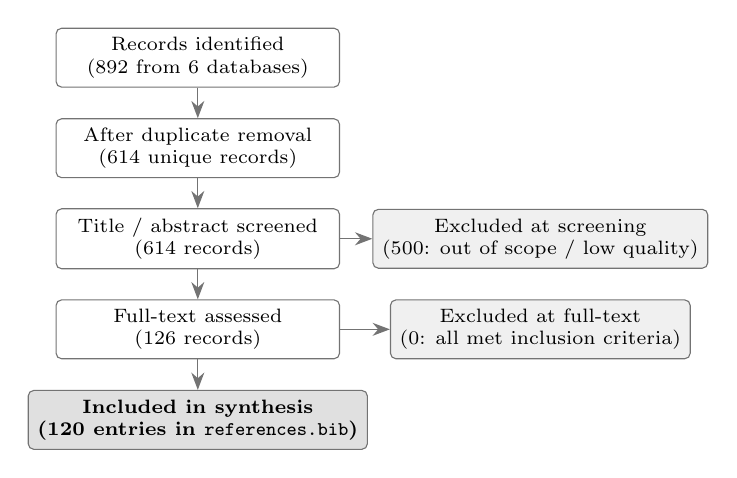
\begin{tikzpicture}[prisma/.style={draw=black!55, fill=white, rounded corners=2pt, minimum width=3.6cm, minimum height=0.72cm, align=center, font=\scriptsize}, prismaem/.style={prisma, fill=black!6, minimum width=3.0cm, minimum height=0.58cm}, arr/.style={-{Stealth[length=2.2mm]}, line width=0.45pt, draw=black!55}
]
  \node[prisma] (id) at (0,0) {Records identified\\(892 from 6 databases)};
  \node[prisma] (dedup) at (0,-1.15) {After duplicate removal\\(614 unique records)};
  \node[prisma] (screen) at (0,-2.3) {Title / abstract screened\\(614 records)};
  \node[prismaem] (excl1) at (4.35,-2.3) {Excluded at screening\\(500: out of scope / low quality)};
  \node[prisma] (full) at (0,-3.45) {Full-text assessed\\(126 records)};
  \node[prismaem] (excl2) at (4.35,-3.45) {Excluded at full-text\\(0: all met inclusion criteria)};
  \node[prisma, fill=black!12, font=\scriptsize\bfseries] (incl) at (0,-4.6)
    {Included in synthesis\\(120 entries in \texttt{references.bib})};
  \draw[arr] (id) -- (dedup);
  \draw[arr] (dedup) -- (screen);
  \draw[arr] (screen) -- (full);
  \draw[arr] (full) -- (incl);
  \draw[arr] (screen.east) -- (excl1.west);
  \draw[arr] (full.east) -- (excl2.west);
\end{tikzpicture}
\caption[PRISMA-style literature screening flow]{PRISMA-style literature screening flow}
\label{fig:prisma-flow}
\end{figure}

\begin{table}[H]
\centering
\footnotesize
\setlength{\tabcolsep}{4pt}
\renewcommand{\arraystretch}{1.12}
\caption[Top-10 ranked literature sources]{Top-10 ranked literature sources}
\label{tab:lit-top10}
\resizebox{\textwidth}{!}{%
\begin{tabular}{@{}cp{4.2cm}p{7.4cm}@{}}
\toprule
\tableheadcolor
\tableheadfont \# & \tableheadfont Source / Module / Operationalized In & \tableheadfont Headline Finding \\
\midrule
1 & Werner et al.\ 2022 [1] · DeFi mechanics · Ch.~3 & DeFi lending is uniformly flat, pool-based, overcollateralized \\
\rowcolor{RowShade}
2 & Tan 2023 (IMF) [5] · CBDC \& hierarchy · Ch.~3 & Two-tier CBDC distribution (central bank $\to$ commercial banks $\to$ users); hierarchical infrastructure is the key design choice \\
3 & Palaiokrassas et al.\ 2024 [3] · Fraud detection · Sec.~\ref{sec:aiml-support} & Multi-chain ML on 54M tx, F1 0.76--0.85 with behavioral features \\
\rowcolor{RowShade}
4 & Adom et al.\ 2022 [4] · Explainable AI · Sec.~\ref{sec:aiml-support} & SHAP outperforms LIME on lending datasets \\
5 & Weber et al.\ 2019 / Elliptic [85] · Graph fraud · Sec.~\ref{sec:gnn-extension} & Graph-structured fraud signal in BTC transactions \\
\rowcolor{RowShade}
6 & McMahan et al.\ 2017 / FedAvg [68] · Federated learning · Sec.~\ref{sec:fl-fraud} & Privacy-preserving model averaging across institutions \\
7 & BIS WP 905 [61] · Stablecoin risk · Secs.~\ref{sec:stablecoin-first}, \ref{sec:mica-compliance} & Algorithmic stablecoins unsuitable for EM DeFi; USDC/USDT recommended \\
\rowcolor{RowShade}
8 & Atzei et al.\ 2017 [7] · Smart contract security · Sec.~\ref{sec:defense-in-depth} & SoK of EVM attack vectors \\
9 & EU MiCA + GENIUS Act [75, 77] · Regulation · Sec.~\ref{sec:mica-compliance} & Stablecoin issuer authorization, reserve disclosure \\
\rowcolor{RowShade}
10 & Bangladesh Bank SP2025-02 [80] · MFI precedent · Sec.~\ref{sec:over-indebt} & Female-to-male account parity 49\%/49\% in 2025; 89\% BRAC loans to women \\
\bottomrule
\end{tabular}%
}
\end{table}

\section{Review of Existing Research}
\label{sec:review-existing}

This chapter surveys peer-reviewed work, institutional reports, and industry data across twelve domains that shape the Crypto World Bank design: DeFi lending, ML fraud detection and explainable AI, hierarchical development finance and cross-tier flows, group/microfinance literature, smart-contract security, gas and Layer~2 scalability, correspondent banking, retail payments and remittance, monetary-policy distributional effects, real-world asset tokenization, stablecoin regulation and institutional settlement rails, and optional LLM/MCP interfaces.

\subsection{Decentralized Lending and DeFi Protocol Design}

DeFi lending automates deposit funding and credit allocation through public smart contracts: utilization curves set rates, oracles trigger liquidations, and settlement is atomic. The model's strengths---real-time auditability, per-block interest, reduced loan-officer discretion---come with structural limits for development finance: participants are fungible (no institutional roles), borrowing is over-collateralized (excluding many unbanked adults), and capital flows one way through flat pools with no inter-tier allocation or multi-entity co-funding.

Werner et al.~[1] systematize DeFi as homogeneous, pool-based, and over-collateralized with no institutional hierarchy---the core gap this thesis addresses. Bastankhah et al.~[2] show adaptive dual fast/slow rate control outperforming static Aave/Compound curves~[51], informing the kinked-rate model (Section~\ref{sec:kinked-rate}). Chen et al.~[39] validate multi-chain lending for throughput; Yang and Cui~[40] supply evaluation metrics (utilization stability, liquidation efficiency, rate responsiveness). Hartmann and Hasan~[41] analyse gas and identity in P2P lending; Dao et al.~[52] adapt credit scoring to DeFi borrowing limits.

\subsection{Machine Learning, Explainable AI, and Extended AI Security}

Palaiokrassas et al.~[3] achieve F1 0.76--0.85 on 54M multi-chain DeFi transactions using behavioral features versus 0.08 with raw transaction data alone---direct input to Random Forest feature engineering. Liu et al.~[6] supply Isolation Forest for unsupervised detection when labeled fraud is scarce. Hasan et al.~[42] train fraud classifiers via federated learning on encrypted features, informing cross-bank intelligence without raw data sharing.

Adom et al.~[4] find SHAP more consistent than LIME for loan explanations; Yuan~[49] reaches AUC $>$0.92 with SHAP on credit-default models---motivating SHAP waterfall review before approvals. Beyond the core pipeline, graph features from Palaiokrassas et al.~[3] support GNN ring detection; federated learning~[42] suits National/Local Bank boundaries; ContractWard~[43] and SoliAudit~[44] enable real-time exploit monitoring; RL rate tuning and NLP income extraction remain future-work options.

\subsection{Hierarchical Distribution, Cross-Tier Flows, and Group Lending}
\label{sec:lit-cross-tier}

Tan~[5] models two-tier CBDC distribution (central bank $\to$ commercial banks $\to$ users), paralleling the four-tier hierarchy. BIS~[46] prefers two-level retail CBDC with interoperability constraints, informing the dual-currency facility. Asaduzzaman et al.~[47] report up to 60\% admin-cost reduction from smart-contract microcredit---literature precedent for \texttt{GroupLendingPool}, not a deployment-jurisdiction claim.

Policy literature establishes hierarchical distribution but sparse programmable \emph{multi-directional} coordination. Kiff et al.~[106] distinguish multi-tier CBDC with supervised intermediaries; Bindseil~[105] analyses tiered remuneration for \texttt{UpwardDepositFacility} rate spreads (Section~\ref{sec:upward-flow}); Auer and B\"{o}hme~[107] hybrid CBDC mirrors client-via-Local-Bank access with Tier~1 reserve authority. \textit{Project Pine}~[103] validates layered contract factories for reserve and collateral dependencies extended by \texttt{InterBankLendingPool} and \texttt{SyndicatedLoan}. Dong et al.~[104] model cross-tier direct financing in supply chains---parallel to downward allocation to capital-constrained retail clients (Figure~\ref{fig:cross-tier-lending}).

Grameen/BRAC solidarity groups achieve $>$95\% repayment through social monitoring that on-chain mutual liability cannot fully replicate; \texttt{GroupLendingPool} encodes multi-signature consent and pool claims at pre-thesis stage. G\"{u}\c{c}\"uk et al.~[53] review privacy and trust in blockchain microlending.

\subsection{Smart Contract Security and Layer~2 Scalability}

Atzei et al.~[7] catalogue reentrancy, access-control, and overflow vectors---motivating OpenZeppelin guards, Solidity~0.8.20, RBAC, Slither, Mythril, and Phase~IV formal verification. Wang et al.~[43] (ContractWard) reach F1 0.96/0.93 on bytecode vulnerability classes; Liao et al.~[44] (SoliAudit) cut audit time $\approx$70\% via ML-prioritized fuzzing; So et al.~[45] (VERISMART) report 98.4\% precision with zero false positives on arithmetic safety---candidate for reserve-ratio invariants.

Kim and Kim~[48] show batching and calldata compression save 30--50\% mainnet gas, supporting Polygon zkEVM Cardona deployment where multi-step four-tier lifecycles multiply savings.

\subsection{Correspondent Banking, Retail Payments, and Settlement Rails}
\label{sec:lit-retail-payments}

BIS~[16] and FSB~[27] document nostro/vostro idle capital, MT103 routing, and 2--5-day settlement. World Bank remittance data~[20] average 6.49\% on a \$200 transfer (Sub-Saharan Africa $>$8\%). Cerutti et al.~[116] and Du et al.~[110] show digital and stablecoin rails can undercut legacy costs but depend on corridor off-ramp depth---scoped separately (Section~\ref{sec:future-retail-payments}).

Retail literature examines stablecoin remittance, merchant checkout, and on/off-ramps for post-MVT modules (\texttt{CurrentAccount}, \texttt{P2PTransfer}). Ante~[108] finds 26\% U.S.\ remittance-user stablecoin adoption, supporting tiered KYC gating. Du et al.~[110] document the fiat--stablecoin--fiat ``sandwich'' pattern. Li et al.~[109] (\textbf{CLEAR} framework) find programmable settlement advantages but weak open-loop dispute recourse; Zhang et al.~[112] warn on refund volatility; Fr\"{o}hlich et al.~[111] show on-ramp friction dominates POS UX. Lin et al.~[113] (\textit{SecurePay}) and BIS \textit{Project Sela}~[119] validate Local-Bank--sponsored multi-intermediary flows; Cimaszewski et al.~[118] blueprint jurisdictional DLT settlement. CPMI~[114], BIS Papers~170~[115], and FATF~[117] define ramp and VASP compliance for platform-mediated \texttt{P2PTransfer}---not permissionless unhosted-wallet remittance. No prior work composes four-tier development-finance lending with closed-loop retail rails in one architecture.

\subsection{Monetary Policy, Tokenization, and Institutional Landscape}
\label{sec:lit-institutional}

Cross-country evidence links QE to wealth inequality~[28]; Federal Reserve metro analysis~[29] shows low-income harm from tightening---motivating algorithmic, transparent rate and reserve parameters rather than opaque committee discretion. Tier-uniform utilization rates reduce loan-officer price discrimination; the Cantillon effect does not apply where USDC is fully reserved and the platform creates no new money~[30].

R3 Corda reports \$17B tokenized RWAs~[31]; Centrifuge exceeds \$1B across eight chains~[32]; World Bank FundsChain tracks disbursements on 13 projects scaling to 250~[33]---institutional precedent for hierarchical on-chain finance beyond fund tracking alone.

Sygnum~[65] notes institutional allocators require legal enforceability (Aave Arc $\approx$\$50k TVL). mBridge~[78] and \textit{Project Agora}~[79] are settlement rails, not retail lending hierarchies; 94\% of central banks research CBDCs~[71]. CWB positions as a lending-layer specification compatible with these rails.

\subsection{Graph ML, Federated Learning, Regulation, and Identity Primitives}

DeFi fraud is relational: Cheng et al.~[93], Chang et al.~[93], and DeFiGuard~[67] outperform flat ML on graph structure---motivating a GNN extension with hierarchical tier edges (Section~\ref{sec:gnn-extension}). Federated learning~[42, 97] and PrivChain-AI (94.7\% accuracy) suit banks that cannot share raw records; FedAvg aggregation at National tier is architecturally natural (Section~\ref{sec:fl-fraud}).

MiCA~[75, 76] and the U.S.\ GENIUS Act~[77] anchor stablecoin-first retail design (Section~\ref{sec:stablecoin-first}; mapping in Section~\ref{sec:mica-compliance}). Buterin et al.~[69] introduce non-transferable SBTs for portable credit passports~[70] (Section~\ref{sec:credit-passport}).

\subsection{Oracle-Mediated ML and Optional LLM Interfaces}
\label{sec:lit-llm}

Luo et al.~[94] survey AI fraud detection across the DeFi lifecycle; Caldarelli~[95] identifies ML-score oracle delivery as under-researched beyond price feeds. BCCC-DeFiFraudTrans-2025~[83] (1,026,867 labeled transactions) is the planned primary training corpus after pre-thesis 2 (Section~\ref{sec:ml-workload}); Fazliani et al.~[96] and Alhasawi et al.~[97] supply semi-supervised and federated baselines.

The optional conversational add-on uses an 8B open-weight LLM with QLoRA, RAG, and refusal layers. Finance LLM studies~[72, 73, 74] report productivity gains but document regulatory-hallucination risks---motivating the red-team protocol in Section~\ref{sec:llm-eval}.

\section{Literature Review Summary}

Table~\ref{tab:lit-summary} (Parts A--F) summarizes reviewed works by methodology, findings, and project relevance, following the synthesis table format recommended by Michigan State University Libraries~[17].

\begin{table}[H]
\centering
\footnotesize
\setlength{\tabcolsep}{4pt}
\renewcommand{\arraystretch}{1.12}
\caption[Literature review summary (Part A)]{Literature review summary (Part A)}
\resizebox{\textwidth}{!}{%
\begin{tabular}{@{}>{\raggedright\arraybackslash}p{3.4cm}>{\raggedright\arraybackslash}p{3.0cm}>{\raggedright\arraybackslash}p{3.8cm}>{\raggedright\arraybackslash}p{3.5cm}@{}}
\toprule
\tableheadcolor
\tableheadfont Author \& Focus & \tableheadfont Methodology & \tableheadfont Key Findings & \tableheadfont Relevance to Our Project \\
\midrule
Palaiokrassas et al.\ (2024) [3] · DeFi fraud detection & XGBoost, NN classifiers on 54M+ multi-chain transactions & F1: 0.76--0.85 vs.\ 0.08 with features alone & Informs Random Forest fraud modeling \\
Adom et al.\ (2022) [4] · XAI in loan approval & LIME / SHAP comparison on lending datasets & SHAP provides deeper, more consistent explainability; LIME is faster & Justifies SHAP as our primary explainability method \\
Tan (2023) [5] · CBDC hierarchical distribution & Model for developing nations & Two-tier CBDC distribution (central bank $\to$ commercial banks $\to$ users); hierarchical infrastructure is the decisive design choice & Informs four-tier architecture and dual-currency facility \\
Liu et al.\ (2008) [6] · Anomaly detection & Isolation Forest on synthetic and real datasets & Isolation via recursive partitioning; shorter paths & Specified as secondary unsupervised detection for wallet behaviour \\
Atzei et al.\ (2017) [7] · Smart contract security & SoK of Ethereum attack vectors & Over-reliance, access control vulnerabilities & Directly informs our security primitives and planned formal verification \\
\bottomrule
\end{tabular}%
}
\TableScreenshotEnd[tab:lit-summary]{Literature Review Summary (Part 1): DeFi Lending and Hierarchical Architecture}
\end{table}

\begin{table}[H]
\centering
\footnotesize
\setlength{\tabcolsep}{4pt}
\renewcommand{\arraystretch}{1.12}
\caption[Literature review summary (Part B)]{Literature review summary (Part B)}
\resizebox{\textwidth}{!}{%
\begin{tabular}{@{}>{\raggedright\arraybackslash}p{3.4cm}>{\raggedright\arraybackslash}p{3.0cm}>{\raggedright\arraybackslash}p{3.8cm}>{\raggedright\arraybackslash}p{3.5cm}@{}}
\toprule
\tableheadcolor
\tableheadfont Author \& Focus & \tableheadfont Methodology & \tableheadfont Key Findings & \tableheadfont Relevance to Our Project \\
\midrule
Werner et al.\ (2022) [1] · DeFi protocol systematisation & SoK survey of 12+ DeFi protocol categories & Lending platforms are uniformly pool-based and overcollateralised; no institutional hierarchy exists & Identifies the core gap our four-tier architecture addresses \\
Bastankhah et al.\ (2024) [2] · Adaptive DeFi lending & Dual fast/slow control; simulation on historical data & Dynamic rate adjustment outperforms static utilisation curves & Validates algorithmic lending parameter optimisation \\
\bottomrule
\end{tabular}%
}
\TableScreenshotEnd{Literature Review Summary (Part 2): Governance, Settlement, and Institutional Adoption}
\end{table}

\begin{table}[H]
\centering
\footnotesize
\setlength{\tabcolsep}{4pt}
\renewcommand{\arraystretch}{1.12}
\caption[Literature review summary (Part C)]{Literature review summary (Part C)}
\resizebox{\textwidth}{!}{%
\begin{tabular}{@{}>{\raggedright\arraybackslash}p{3.4cm}>{\raggedright\arraybackslash}p{3.0cm}>{\raggedright\arraybackslash}p{3.8cm}>{\raggedright\arraybackslash}p{3.5cm}@{}}
\toprule
\tableheadcolor
\tableheadfont Author \& Focus & \tableheadfont Methodology & \tableheadfont Key Findings & \tableheadfont Relevance to Our Project \\
\midrule
Hartmann and Hasan (2021) [41] · Blockchain P2P lending & Smart contract-mediated loan origination framework & Eliminates intermediary overhead; gas cost minimisation analysis & Informs four-tier architecture for peer-to-peer lending \\
Hasan et al.\ (2022) [42] · Privacy-preserving fraud detection & Federated learning on encrypted blockchain features & ML achieves comparable accuracy to centralised models & Informs future privacy-preserving fraud detection extensions \\
Wang et al.\ (2020) [43] · Smart contract vulnerability detection & ML classifiers on bytecode features & F1: 0.96 for access control; 0.93 for data leakage & Supports our planned security verification models \\
Liao et al.\ (2019) [44] · Smart contract audit automation & Hybrid classification + fuzz testing & Reduces audit time by 70\% vs.\ manual review & Informs our security audit strategy for three-contract architecture \\
\bottomrule
\end{tabular}%
}
\TableScreenshotEnd{Literature Review Summary (Part 3): Cross-Border Settlement and Security Tooling}
\end{table}

\begin{table}[H]
\centering
\footnotesize
\setlength{\tabcolsep}{4pt}
\renewcommand{\arraystretch}{1.12}
\caption[Literature review summary (Part D)]{Literature review summary (Part D)}
\resizebox{\textwidth}{!}{%
\begin{tabular}{@{}>{\raggedright\arraybackslash}p{3.4cm}>{\raggedright\arraybackslash}p{3.0cm}>{\raggedright\arraybackslash}p{3.8cm}>{\raggedright\arraybackslash}p{3.5cm}@{}}
\toprule
\tableheadcolor
\tableheadfont Author \& Focus & \tableheadfont Methodology & \tableheadfont Key Findings & \tableheadfont Relevance to Our Project \\
\midrule
BIS et al.\ (2020) [46] · CBDC design requirements & Analysis of retail CBDC distribution architecture & Two-tier model preferred; interoperability challenges identified & Informs dual-currency facility design \\
Kiff et al.\ (2020) [106] · CBDC operating models & IMF survey of retail CBDC architectures & Multi-tier models delegate distribution to supervised intermediaries & Supports four-tier wholesale-to-retail capital path \\
Bindseil (2020) [105] · Tiered CBDC remuneration & ECB policy analysis of two-tier CBDC rates & Tiered rates preserve bank intermediation; control disintermediation risk & Informs upward/downward asymmetric rate spread \\
Dong et al.\ (2023) [104] · Cross-tier supply-chain finance & Three-tier game-theoretic MSOM model & Blockchain cross-tier direct financing reaches capital-constrained deep tiers & Parallel to downward client lending without wholesale bypass \\
Project Pine (2025) [103] · Hierarchical smart contracts & NY Fed / BIS tokenized policy toolkit prototype & Factory-to-facility contract hierarchy for reserves and collateral & Validates layered contract design for \texttt{IBLP} / \texttt{SyndicatedLoan} \\
BIS/FSB [16] · Cross-border settlement infrastructure & Analysis of cross-border payment costs and capital trapped in nostro accounts & 2--5 days avg.\ settlement; \$42/transfer avg.\ cost & Motivates four-tier settlement with near-instant finality \\
Beyer et al.\ (2025) [28] · Monetary policy and inequality & Cross-country analysis (1999--2019) & QE increases wealth inequality; effects more persistent than monetary parameters & Motivates transparent, algorithmic monetary parameters \\
World Bank (2025) [33] · Blockchain for development finance & Pilot on 13 projects, 10 countries & Blockchain tracking reduces reporting burden for fund distribution & Supports our planned multi-chain deployment strategy \\
\bottomrule
\end{tabular}%
}
\TableScreenshotEnd{Literature Review Summary (Part 4): Risk Monitoring and AI/ML in Finance}
\end{table}

\begin{table}[H]
\centering
\footnotesize
\setlength{\tabcolsep}{4pt}
\renewcommand{\arraystretch}{1.12}
\caption[Literature review summary (Part E)]{Literature review summary (Part E)}
\resizebox{\textwidth}{!}{%
\begin{tabular}{@{}>{\raggedright\arraybackslash}p{3.4cm}>{\raggedright\arraybackslash}p{3.0cm}>{\raggedright\arraybackslash}p{3.8cm}>{\raggedright\arraybackslash}p{3.5cm}@{}}
\toprule
\tableheadcolor
\tableheadfont Author \& Focus & \tableheadfont Methodology & \tableheadfont Key Findings & \tableheadfont Relevance to Our Project \\
\midrule
Chen et al.\ (2024) [39] · Multi-chain DeFi lending & Cross-chain model design and implementation & Multi-chain distribution improves throughput and reduces congestion & Supports our planned multi-chain deployment strategy \\
Yang and Cui (2023) [40] · DeFi lending protocol evaluation & Quantitative risk metrics for lending protocol assessment & Utilisation ratio, liquidation efficiency, and reserve responsiveness as key metrics & Provides benchmarks for evaluating our hierarchical tiers \\
Asaduzzaman et al.\ (2020) [47] · Smart micro-credit (MFI literature) & Smart contract-based microfinance & Reduces admin overhead by 60\% vs.\ manual processes & Informs \texttt{GroupLendingPool} economic case \\
Kim and Kim (2024) [48] · DeFi gas fee optimisation & Transaction batching and calldata compression analysis & Gas savings of 30--50\% through optimisation strategies & Validates Layer~2 deployment and mainnet optimisation \\
Yuan (2024) [49] · SHAP-based credit default models & SHAP, Random Forest, and Gradient Boosting classifiers & AUC above 0.92 with full interpretability & Informs per-client risk explanation methodology \\
\bottomrule
\end{tabular}%
}
\TableScreenshotEnd{Literature Review Summary (Part 5): Institutional Adoption and MFI Literature}
\end{table}

\begin{table}[H]
\centering
\footnotesize
\setlength{\tabcolsep}{4pt}
\renewcommand{\arraystretch}{1.12}
\caption[Literature review summary (Part F)]{Literature review summary (Part F)}
\resizebox{\textwidth}{!}{%
\begin{tabular}{@{}>{\raggedright\arraybackslash}p{3.4cm}>{\raggedright\arraybackslash}p{3.0cm}>{\raggedright\arraybackslash}p{3.8cm}>{\raggedright\arraybackslash}p{3.5cm}@{}}
\toprule
\tableheadcolor
\tableheadfont Author \& Focus & \tableheadfont Methodology & \tableheadfont Key Findings & \tableheadfont Relevance to Our Project \\
\midrule
Ante (2025) [108] · Stablecoin remittance adoption & Survey ($n{=}866$) of U.S.\ remittance users & 26\% stablecoin adoption; literacy drives uptake; continuance tied to usefulness & Informs KYC ladder and UX for \texttt{P2PTransfer} \\
Du et al.\ (2026) [110] · Competing payment rails & Harmonized all-in cost comparison across corridors & Stablecoin sandwich can undercut banks/MTOs; off-ramp depth is binding & Motivates PSP on/off-ramp future work \\
Li et al.\ (2026) [109] · Stablecoin retail payments SoK & CLEAR framework vs.\ card networks & Closed-loop / cross-border advantage; weak open-loop dispute recourse & Frames merchant checkout and \texttt{InsuranceFund} design \\
Zhang et al.\ (2024) [112] · Retail stablecoin checkout & Analytical operations model & Stablecoin refunds create consumer volatility disutility & Supports fiat-display \texttt{FXModule} and auto-conversion \\
Fr\"{o}hlich et al.\ (2022) [111] · Crypto POS usability & Mixed-methods Lightning checkout study & Friction at on-ramp, not tap-to-pay & Prioritises fiat-funded \texttt{CurrentAccount} balances \\
Lin et al.\ (2025) [113] · Platform-economy payments & Permissioned chain + regulated money prototype & $\approx$256~TPS; multi-intermediary escrow & Parallel to Local-Bank--sponsored merchant flows \\
CPMI / BIS [114, 115] · Stablecoin policy & Cross-border and monetary-system analysis & On/off-ramps gate acceptance; reserve transparency critical & Regulatory anchor for ramp integration \\
FATF (2021) [117] · VASP / P2P guidance & Risk-based AML standards for virtual assets & Platform-mediated transfers require originator data; pure unhosted P2P out of scope & Compliance model for sponsored \texttt{P2PTransfer} \\
\bottomrule
\end{tabular}%
}
\TableScreenshotEnd{Literature Review Summary (Part 6): Retail Payments and Remittance Rails}
\end{table}

\section{Comparative Protocol Analysis}
\label{sec:comparative-protocol}

No surveyed protocol combines multi-tier hierarchy, oracle-mediated explainable ML, and compliance-aware identity. Table~\ref{tab:protocol-comparison} compares CWB against Aave, Compound, Maker, Maple, and Goldfinch on eleven architectural dimensions.

\begin{table}[H]
\centering
\footnotesize
\setlength{\tabcolsep}{3pt}
\resizebox{\textwidth}{!}{%
\begin{tabular}{@{}p{3.4cm}*{6}{>{\centering\arraybackslash}p{1.35cm}}@{}}
\toprule
\tableheadcolor
\tableheadfont Feature & \tableheadfont Aave & \tableheadfont Comp. & \tableheadfont Maker & \tableheadfont Maple & \tableheadfont Gfinch & \tableheadfont CWB \\
\midrule
Institutional hierarchy & \tmarkNo{} & \tmarkNo{} & \tmarkNo{} & \tmarkNo{} & \tmarkNo{} & \tmarkPlanned{} \\
\rowcolor{RowShade}
Cross-tier capital flow & \tmarkNo{} & \tmarkNo{} & \tmarkNo{} & \tmarkNo{} & \tmarkNo{} & \tmarkPartial{} \\
Same-tier interbank lending & \tmarkNo{} & \tmarkNo{} & \tmarkNo{} & \tmarkNo{} & \tmarkNo{} & \tmarkPartial{} \\
\rowcolor{RowShade}
Syndicated / co-lending & \tmarkNo{} & \tmarkNo{} & \tmarkNo{} & Part. & Part. & \tmarkPartial{} \\
Upward capital repatriation & \tmarkNo{} & \tmarkNo{} & \tmarkNo{} & \tmarkNo{} & \tmarkNo{} & \tmarkPartial{} \\
\rowcolor{RowShade}
Solidarity group lending & \tmarkNo{} & \tmarkNo{} & \tmarkNo{} & \tmarkNo{} & Part. & \tmarkPlanned{} \\
AI/ML fraud detection & \tmarkNo{} & \tmarkNo{} & \tmarkNo{} & Man. & Man. & \tmarkPlanned{} \\
\rowcolor{RowShade}
SHAP explainability & \tmarkNo{} & \tmarkNo{} & \tmarkNo{} & \tmarkNo{} & \tmarkNo{} & \tmarkPlanned{} \\
ZKP KYC compliance & \tmarkNo{} & \tmarkNo{} & \tmarkNo{} & \tmarkNo{} & \tmarkNo{} & \tmarkPlanned{} \\
\rowcolor{RowShade}
Kinked interest rate curve & \tmarkDone{} & \tmarkDone{} & Gov. & \tmarkDone{} & \tmarkNo{} & \tmarkPartial{} \\
Role-based access control & Part. & Part. & Gov. & \tmarkDone{} & Part. & \tmarkPlanned{} \\
\rowcolor{RowShade}
Institutional / L2 focus & \tmarkNo{} & \tmarkNo{} & \tmarkNo{} & \tmarkDone{} & Part. & \tmarkPlanned{} \\
TVL / Status (2026) & \$26B & \$1.4B & \$10B & \$2.6B & \$680M & Planning \\
\bottomrule
\end{tabular}%
}
\caption[Protocol comparison on eleven architectural dimensions]{Protocol comparison on eleven architectural dimensions}
\label{tab:protocol-comparison}
\end{table}

This answers RQ1: Aave~v3 and Compound~v3 sub-markets differentiate assets within flat pools, not institutional relationships or inter-bank flows; Maple, Goldfinch, and Morpho~V2~[117, 90] lack multilateral development-finance capital allocation. CWB's compound novelty (Section~\ref{sec:research-contribution}) holds across hierarchy, explainable ML governance, and group lending axes.

\paragraph{ERC-3643 (T-REX) alignment.}
Tiers~1--3 use bespoke RBAC (Section~\ref{sec:defense-in-depth}) functionally equivalent to ERC-3643 token-level KYC gating~[82]; production under MiCA~[75] could migrate to full T-REX interoperability without redesigning the role registry.

\paragraph{Contrast with opaque custody failures.}
FTX's 2022 collapse exposed commingled client funds with no real-time solvency proof---the class of failure CWB addresses via enforced per-tier reserve ratios readable on-chain. The platform targets banking (savings, credit, interbank lending), not speculative exchange activity.

\subsection{Literature Synthesis}

Six design decisions follow directly from the survey: (1)~Gudgeon et al.~[56] on utilization crises $\to$ kinked-rate model (Section~\ref{sec:kinked-rate}); (2)~Piper et al.~[58] $\to$ ZKP identity path (Section~\ref{sec:identity}); (3)~Tan~[5], BIS~[46], Kiff~[106], Auer and B\"{o}hme~[107] $\to$ four-tier capital flows; (4)~Bindseil~[105], Project Pine~[103], Dong et al.~[104] $\to$ multi-directional lending (Section~\ref{sec:cross-tier-lending}); (5)~Asaduzzaman et al.~[47] $\to$ \texttt{GroupLendingPool}; (6)~Ante~[108], Du et al.~[110], Li et al.~[109], Lin et al.~[113], CPMI~[114], FATF~[117] $\to$ post-MVT retail stack (Section~\ref{sec:future-retail-payments}).

\subsection{Agent Harness Engineering and Production Safety}
\label{sec:harness-lit}

Alizadeh et al.~[87] show income uploads and language-preference fields as prompt-injection vectors in banking agents---fields present in CWB context assembly. OWASP LLM Top~10~[88] ranks prompt injection (LLM01) highest for agentic finance, framing evaluation of the scanning middleware.

\section{Summary of Key Findings}
\label{sec:lit-key-findings}

The literature review yields the following design-relevant conclusions:

\begin{itemize}[noitemsep]
\item \textbf{Flat DeFi vs.\ tiered finance.} Pool-based protocols exceed \$55B TVL~[8] but lack institutional hierarchy; CBDC research confirms tiered distribution as a workable pattern~[5]. No prior work models four-tier reserve-enforced lending.
\item \textbf{Settlement and retail rails.} Correspondent banking traps idle capital~[18], settles in 2--5 days at $\approx$\$42/transfer~[19], and costs remittance users \$48--56B annually~[20]. Stablecoin rails can compress costs~[116, 110] but need ramp infrastructure; retail studies~[109, 112, 111, 113, 119] favour Local-Bank--sponsored closed-loop flows over open permissionless checkout.
\item \textbf{ML, XAI, and security.} Behavioral DeFi features lift fraud F1 to 0.76--0.85~[3]; Isolation Forest~[6] covers unlabeled cases; SHAP beats LIME for regulatory explainability~[4]. Contract vulnerabilities are well catalogued~[7]; ML audit tools reach F1 $>$0.93~[43], cut review time 70\%~[44], and formal verifiers such as VERISMART reach 98.4\% precision~[45].
\item \textbf{Hierarchy, groups, and institutions.} Cross-tier CBDC and Project Pine literature~[106, 105, 107, 103, 104] supports multi-directional programmable flows; analogue MFIs report $>$95\% group repayment~[47] with on-chain mutual liability still an open gap. FundsChain~[33], Corda RWAs~[31], and Kinexys~[34] show rising institutional blockchain adoption.
\item \textbf{Scalability, privacy, and regulation.} Multi-chain lending~[39] and L2 gas optimization~[48] cut costs 30--50\%; federated learning~[42, 97] enables cross-bank fraud intelligence without raw data sharing. MiCA and GENIUS~[75, 77] anchor stablecoin-first design; algorithmic parameters mitigate distributional opacity from discretionary monetary policy~[28, 29].
\item \textbf{Deposit-funded sustainability.} Sustainable MFIs rely on mobilized deposits, not donor capital alone---motivating savings vaults at the Local Bank tier alongside \texttt{GroupLendingPool}.
\end{itemize}

These findings justify the four-tier architecture, cross-tier lending modules, Random Forest / Isolation Forest / SHAP analytics, governance structure, and phased security verification pipeline developed in later chapters.

%% CHAPTER 3: SYSTEM ARCHITECTURE AND DESIGN
\chapter{System Architecture and Design}

\section{Prototype Scope}
\label{sec:prototype-scope}

\begin{table}[H]
\centering
\caption[Prototype scope and implementation status]{Prototype scope and implementation status}
\label{tab:prototype-scope}
\footnotesize
\renewcommand{\arraystretch}{0.88}
\setlength{\tabcolsep}{3pt}
\begin{tabular}{@{}p{7.1cm}>{\raggedleft\arraybackslash}p{5.9cm}@{}}
\toprule
\tableheadcolor
\tableheadfont Feature & \tableheadfont Status \\
\midrule
Four-tier role system (RBAC) & \tmarkPartial{} Specified \\
\rowcolor{RowShade}
World Bank Reserve contract (Tier~1) & \tmarkPartial{} Specified (Phase~I) \\
Tier~2 National Bank contracts & \tmarkPartial{} Specified (Phase~I) \\
\rowcolor{RowShade}
Tier~3 Local Bank contracts & \tmarkPartial{} Specified (Phase~I) \\
Cross-tier fund transfer & \tmarkPlanned{} Planned (Phase~II) \\
\rowcolor{RowShade}
Loan request / approval workflow & \tmarkPartial{} Specified (Phase~II) \\
Installment EMI auto-generation & \tmarkPlanned{} Planned (Phase~II) \\
\rowcolor{RowShade}
SavingsVault contract & \tmarkPlanned{} Planned (Phase~II) \\
FixedDeposit contract & \tmarkPlanned{} Planned (Phase~II) \\
\rowcolor{RowShade}
GroupLendingPool contract & \tmarkPlanned{} Planned (Phase~II) \\
InterBankLendingPool & \tmarkPlanned{} Planned (Phase~II) \\
\rowcolor{RowShade}
AI/ML fraud detection (Random Forest) & \tmarkPlanned{} Planned (Phase~III) \\
SHAP + anomaly explainability & \tmarkPlanned{} Planned (Phase~III) \\
\rowcolor{RowShade}
Oracle integration (Chainlink Functions) & \tmarkPlanned{} Planned (Phase~III) \\
ZKP KYC compliance layer & \tmarkPlanned{} Planned (Phase~IV) \\
\rowcolor{RowShade}
Testnet deployment (Polygon zkEVM Cardona) & \tmarkPlanned{} Planned (Phase~IV) \\
AI Agent / MCP tool server (17 tools) & \tmarkPlanned{} Optional (Phase~III--IV) \\
\rowcolor{RowShade}
EIP-7702 session key management & \tmarkPlanned{} Optional (Phase~III) \\
Authority Brief UI (SHAP for approvers) & \tmarkPlanned{} Planned (Phase~III) \\
\rowcolor{RowShade}
Chainlink Automation (installment triggers) & \tmarkPlanned{} Planned (Phase~II) \\
Chainlink Proof of Reserve & \tmarkPlanned{} Planned (Phase~I) \\
\rowcolor{RowShade}
The Graph subgraph (event indexing) & \tmarkPlanned{} Planned (Phase~III) \\
SAR workflow (AML $\to$ freeze queue) & \tmarkPlanned{} Planned (Phase~III) \\
\rowcolor{RowShade}
\texttt{sessions} table schema & \tmarkPartial{} Specified (Phase~I) \\
\texttt{agent\_action\_log} table schema & \tmarkPlanned{} Optional (Phase~III) \\
\rowcolor{RowShade}
300-client Foundry simulation & \tmarkPlanned{} Planned (Phase~IV) \\
\bottomrule
\end{tabular}
\end{table}

\paragraph{Chapter organisation.}
The remainder of this chapter is organised as follows. Sections~\ref{sec:high-level-arch}--\ref{sec:oracle-architecture} describe the platform stack, contract inventory, blockchain selection, and oracle architecture. Sections~\ref{sec:data-model}--\ref{sec:data-partitioning} present the relational data model and on-chain/off-chain partitioning. Sections~\ref{sec:operating-context}--\ref{sec:funnel} cover operating context, identity, onboarding, and the retail conversion funnel. Sections~\ref{sec:kinked-rate}--\ref{sec:bridge} specify interest-rate, liquidation, deposit, credit-passport, and cross-chain designs. Section~\ref{sec:multi-entity} details multi-entity capital operations. Sections~\ref{sec:system-modeling}--\ref{sec:banking-products} provide UML-style models and the banking product suite. Sections~\ref{sec:governance-framework}--\ref{sec:threat-model} close with governance and the five-layer security architecture.

\paragraph{Specification voice.}
Throughout this chapter, \textbf{specified} denotes a formally documented design in pre-thesis 1; \textbf{planned} denotes a Phase~I--IV implementation deliverable after pre-thesis 2; and \textbf{optional} denotes the conversational agent add-on, which mirrors the same Express.js API and smart contracts as the primary React interface but is not required for core platform operation. \textbf{All AI/ML training and live inference begin after pre-thesis 2} (Section~\ref{sec:ml-workload}). Architectural descriptions use the present tense for specification clarity; Table~\ref{tab:prototype-scope} takes precedence when scope could be ambiguous.

\section{High-Level Architecture}
\label{sec:high-level-arch}

The system employs a \textbf{four-layer decentralised application architecture} (Figure~\ref{fig:three-layer-arch}): a presentation layer (React + wallet integration), a smart-contract layer (fifteen modular EVM contracts centred on the four-tier lending hierarchy), an off-chain services layer (Express REST API, PostgreSQL, planned FastAPI ML scoring after pre-thesis 2, Chainlink oracle integration, event listener, and Redis cache), and a Chainlink infrastructure layer (Chainlink Functions, Automation, Price Feeds, and Proof of Reserve). An optional conversational agent (Qwen3-8B + MCP tool server) attaches to the same API endpoints as the React UI and does not alter on-chain logic. Figure~\ref{fig:component-diagram} elaborates this view with external integrations.

\begin{figure}[H]
\centering
\BalancedDiagram{Ch3_four-layer-dapp-architecture.png}
\caption[Four-layer application architecture]{Four-layer application architecture}
\label{fig:three-layer-arch}
\end{figure}

The architecture \textbf{specifies} fifteen modular contracts. Phase~I targets the three-tier lending core (World Bank Reserve, National Bank, Local Bank). The remaining twelve split into two suites: \textit{banking products} (SavingsVault, FixedDeposit, GroupLendingPool, FXModule, InsuranceFund, CurrentAccount) and \textit{multi-entity operations} (InterBankLendingPool, UpwardDepositFacility, SyndicatedLoan, TranchedPool, TreasurySwap, NettingEngine)---the latter enabling same-tier lending, upward funding, syndicated co-lending, treasury FX, and multilateral netting (Section~\ref{sec:multi-entity}, Figure~\ref{fig:multi-entity-ops}). All are planned across Phases~II and~III.

Figure~\ref{fig:component-diagram} shows component interactions. Core lending contracts are specified in Phase~I; extended modules are planned extensions documented in Appendix~B.

\begin{figure}[H]
\centering
\BalancedDiagram{fig-component-architecture.pdf}
\caption[Component diagram (planning phase)]{Component diagram (planning phase)}
\label{fig:component-diagram}
\end{figure}

\begin{table}[H]
\centering
\begin{tabular}{p{3.6cm}p{2.4cm}p{1.8cm}p{6.7cm}}
\toprule
\tableheadcolor
\textbf{Contract} & \textbf{Module} & \textbf{Status} & \textbf{Primary responsibility} \\
\midrule
WorldBankReserve & Tier~1 core & Specified (Phase~I) & Global reserve custody, national-bank registration, downward capital allocation. \\
NationalBank & Tier~2 core & Specified (Phase~I) & Local-bank registration, upward borrowing, downward allocation. \\
LocalBank & Tier~3 core & Specified (Phase~I) & Client onboarding, loan lifecycle, installments, \texttt{freezeAccount}. \\
SavingsVault & Deposits & Specified (Phase~II) & Variable-yield savings, reserve-gated withdrawals. \\
FixedDeposit & Deposits & Specified (Phase~II) & Term deposits with deterministic early-withdrawal penalty. \\
GroupLendingPool & Group credit & Specified (Phase~II) & Solidarity-group formation, consent, mutual liability. \\
FXModule & Treasury / FX & Specified (Phase~II) & Oracle-priced retail FX with disclosed spread. \\
InsuranceFund & Risk buffer & Specified (Phase~II) & Default coverage buffer; Chainlink Proof of Reserve. \\
CurrentAccount & Payments & Specified (Phase~II) & Transactional accounts and atomic peer transfers. \\
InterBankLendingPool & Multi-entity & Specified (Phase~II) & Same-tier interbank liquidity pools per tier. \\
UpwardDepositFacility & Multi-entity & Specified (Phase~II) & Upward surplus repatriation with yield spread. \\
SyndicatedLoan & Multi-entity & Planned (Phase~III) & Multi-lender syndicate consent and disbursement. \\
TranchedPool & Multi-entity & Planned (Phase~III) & Senior/junior tranching and waterfall recovery. \\
TreasurySwap & Multi-entity & Specified (Phase~II) & Institutional oracle-priced asset swaps. \\
NettingEngine & Multi-entity & Planned (Phase~III) & Multilateral settlement netting batches. \\
\bottomrule
\end{tabular}
\TableScreenshotEnd{Smart Contract Inventory: Fifteen Modular Contracts Across Core, Product, and Multi-Entity Modules}
\end{table}

\section{Blockchain Platform Selection}

\begin{figure}[H]
\centering
\BalancedDiagram{fig-blockchain-stack.pdf}
\caption[Layered blockchain and application stack]{Layered blockchain and application stack}
\label{fig:blockchain-stack}
\end{figure}

\begin{table}[H]
\centering
\caption[Blockchain platform selection criteria and justification]{Blockchain platform selection criteria and justification}
\label{tab:blockchain-selection}
\begin{tabular}{p{3.5cm}p{3.5cm}p{6.5cm}}
\toprule
\tableheadcolor
\textbf{Criterion} & \textbf{Selection} & \textbf{Justification} \\
\midrule
Platform & Ethereum Virtual Machine (EVM) & Largest developer ecosystem; battle-tested security model; extensive tooling. \\
Network & Polygon zkEVM Cardona / Ethereum Sepolia & Zero-cost deployment; production-equivalent behaviour; free faucet access. \\
Consensus & ZK validity proofs (Polygon zkEVM L2, Ethereum L1 settlement) & Every batch of transactions is accompanied by a zero-knowledge proof verified on Ethereum L1, so security derives from cryptographic validity rather than a validator set assumption. \\
Smart contract language & Solidity 0.8.20 & Industry standard; mature compiler with overflow protection; rich library ecosystem. \\
\bottomrule
\end{tabular}
\TableScreenshotEnd{Blockchain Platform Selection: Comparison of EVM-Compatible Networks}
\end{table}

\vspace{2pt}

\begin{table}[H]
\centering
\caption[Blockchain platform selection (continued)]{Blockchain platform selection (continued)}
\begin{tabular}{p{3.5cm}p{3.5cm}p{6.5cm}}
\toprule
\tableheadcolor
\textbf{Criterion} & \textbf{Selection} & \textbf{Justification} \\
\midrule
Gas cost & \$0.001--\$0.01 per transaction & Orders of magnitude cheaper than Ethereum mainnet (\$5--\$50); enables micro-loan economics. \\
Block finality & $\approx$2 seconds & Sub-second practical finality for retail UX; checkpointed to Ethereum for security. \\
Developer tooling & Hardhat + OpenZeppelin & Automated test suite, deployment scripts, and audited security primitives. \\
Testnet availability & Cardona (Polygon zkEVM), Sepolia (Ethereum) & Free faucets; EVM-identical behaviour; no real cryptocurrency required for prototype. \\
Security model & ZK validity proofs & Every batch verified by a ZK proof anchored to Ethereum L1 (vs.\ PoS validator assumption on Amoy). \\
Migration path & EVM-compatible & Same Solidity contracts deploy to any EVM chain; reduces future L2 migration cost. \\
\bottomrule
\end{tabular}
\TableScreenshotEnd{Blockchain Platform Selection (Continued): Operational and Deployment Factors}
\end{table}

\vspace{2pt}

\subsection{Transaction Verification and Consensus}

\begin{itemize}[noitemsep]
\item \textbf{Polygon zkEVM Cardona:} ZK validity proofs anchor batches to Ethereum~L1 (cryptographic security vs.\ PoS validator assumption on Amoy).
\item \textbf{On prototype testnets:} Cardona and Sepolia use equivalent consensus models at no financial cost, enabling incremental development and testing without exposure to real-asset risk.
\end{itemize}

\paragraph{Gas-cost sustainability.}
The hierarchical loan lifecycle generates multiple on-chain state transitions per client; on Polygon zkEVM Cardona the \textbf{projected} cost remains well below 0.01\% of interest earned on a representative retail loan (Section~\ref{sec:gas-cost}), to be validated by the Phase~IV Foundry simulation. This margin underpins the micro-loan economics that motivate Layer~2 deployment in the platform selection above.

\subsection{Oracle Architecture: Off-Chain AI to On-Chain Decision}
\label{sec:oracle-architecture}

The Crypto World Bank requires a mechanism to convey off-chain AI/ML risk assessments into the on-chain loan approval workflow. This is an instance of the oracle problem~[54, 55].

\paragraph{Chainlink Functions oracle (primary).}
The final thesis phase uses \textbf{Chainlink Functions} as the primary oracle mechanism. Chainlink Functions operates via a Decentralised Oracle Network (DON): the ML risk score is fetched independently by multiple Chainlink nodes, consensus across the DON is required before the result is committed on-chain, and no single compromised node can manipulate the risk score. This is a fundamental trust improvement over the earlier commit-reveal relay, which required trusting a single FastAPI service key. The source code executed by the DON is:

\begin{verbatim}
// Chainlink Functions source (runs in decentralised DON)
const clientId = args[0];
const response = await Functions.makeHttpRequest({
  url: `https://your-ml-service.com/score/${clientId}`,
  method: "POST"
});
const score = response.data.risk_score;
// 6 decimal precision
return Functions.encodeUint256(Math.round(score * 1e6));
\end{verbatim}

The DON adds 30--60 seconds of latency and \$0.10--\$1.00 per oracle call, both acceptable for the loan approval lifecycle where decisions are not time-critical. This architecture closes the oracle trust assumption noted in the prototype design (the 2-of-3 Safe multisig attestation was the interim mitigation; Chainlink Functions removes the need for that mitigation entirely).

\paragraph{Commit-reveal relay (prototype fallback).}
After pre-thesis 2, during the prototype phase and prior to Chainlink Functions being wired (Phase~III), the system will use a commit-reveal relay as a fallback. The off-chain ML service commits a hash $h = \text{keccak256}(s \,\|\, \text{nonce})$ to the \texttt{LoanController} contract, then reveals $s$ and the nonce within the decision window. The contract verifies $h = \text{keccak256}(s \,\|\, \text{nonce})$ and stores $s$ immutably. This pattern prevents score manipulation between commitment and decision and creates an immutable on-chain audit trail of every risk score used in a lending decision, while Chainlink Functions integration is completed.

\paragraph{Chainlink Automation: trustless installment triggers.}
\textbf{Chainlink Automation} replaces the centralised cron job for overdue installment detection and interest accrual. The entire loan lifecycle from application to overdue flagging runs without a trusted operator:

\begin{verbatim}
// In LocalBankPool.sol
function checkUpkeep(bytes calldata) external view override
    returns (bool upkeepNeeded, bytes memory performData) {
    uint256[] memory overdueLoans = getOverdueLoans();
    upkeepNeeded = overdueLoans.length > 0;
    performData = abi.encode(overdueLoans);
}

function performUpkeep(bytes calldata performData) external override {
    uint256[] memory overdueLoans =
        abi.decode(performData, (uint256[]));
    for (uint i = 0; i < overdueLoans.length; i++) {
        _markInstallmentOverdue(overdueLoans[i]);
    }
}
\end{verbatim}

This removes the last centralised component from the loan lifecycle --- the entire process from application to overdue flagging runs without a trusted operator.

\paragraph{Chainlink Price Feeds: fiat and crypto pairs.}
The \texttt{FXModule} contract uses Chainlink's production-grade \texttt{AggregatorV3Interface} price feeds for ETH/USD, USDC/USD, and governance-selected fiat pairs (e.g.\ EUR/USD), replacing the earlier ``forex oracle approved by governance'' pattern. Optional fiat-equivalent display in the frontend flows through:

\begin{verbatim}
// In LocalBankPool.sol
AggregatorV3Interface internal fiatUsdFeed;  // e.g. EUR/USD
AggregatorV3Interface internal ethUsdFeed;

function getFiatEquivalent(uint256 usdcAmount)
    public view returns (uint256) {
    (, int fiatRate,,,) = fiatUsdFeed.latestRoundData();
    // USDC tracks USD 1:1; Chainlink uses 8 decimals
    return usdcAmount * uint256(fiatRate) / 1e8;
}
\end{verbatim}

The 8-decimal precision convention is the Chainlink standard for fiat-pair feeds. Chainlink price feeds are a planned Phase~I integration for optional fiat-equivalent display in the frontend.

\paragraph{Chainlink Proof of Reserve.}
The \texttt{WorldBankReserve} contract publishes its reserve balance to \textbf{Chainlink Proof of Reserve (PoR)}, making the reserve cryptographically verifiable by any external auditor without trusting CWB's administrator. This is the ``free PoR'' advantage over FTX: any external system can verify reserve solvency without relying on CWB's admin claims.

\begin{verbatim}
// WorldBankReserve.sol
function getReserveSummary() external view returns (
    uint256 totalDeposited,
    uint256 totalLoaned,
    uint256 reserveRatio,   // scaled 1e4 (e.g. 5000 = 50%)
    uint256 insuranceFundBalance
) {
    return (
        totalDeposited,
        totalLoaned,
        (totalDeposited - totalLoaned) * 1e4 / totalDeposited,
        insuranceFund.balance()
    );
}
\end{verbatim}

This function is the FTX commingling safeguard described in Section~\ref{sec:defense-in-depth}. Adding Chainlink's PoR job on top turns it into a market-standard verifiable proof, and it is specified in full in Appendix~D.

\begin{figure}[H]
\centering
\BalancedDiagram{fig-oracle-architecture.pdf}
\caption[Chainlink oracle architecture]{Chainlink oracle architecture}
\label{fig:oracle-architecture}
\end{figure}

\section{Data Model and Database Design}
\label{sec:data-model}

The relational database schema comprises 20 normalized entities in Third Normal Form (3NF). Figure~\ref{fig:core-system-graph} presents the core entity-relationship overview, Figure~\ref{fig:erd-extended} presents extended product and multi-entity entities, and Figure~\ref{fig:eer} presents the Enhanced Entity-Relationship (EER) diagram with specialisation and weak-entity constructs.

\begin{figure}[H]
\centering
\BalancedDiagram{Ch3_core-entity-relationship-diagram.png}
\caption[Core system entity graph]{Core system entity graph}
\label{fig:core-system-graph}
\end{figure}

\begin{figure}[H]
\centering
\BalancedDiagram{Ch3_extended-erd-banking-multi-entity.png}
\caption[Extended ERD entities]{Extended ERD entities}
\label{fig:erd-extended}
\end{figure}

The current ERD covers the core lending and governance entities. Figure~\ref{fig:erd-extended} presents the extended banking entities (SavingsAccount, FixedDeposit, LoanGroup, GroupMember, CurrentAccount, and InsuranceFund) and the multi-entity / cross-tier operational entities described in Section~\ref{sec:multi-entity-consistency}: \texttt{INTERBANK\_LOAN}, \texttt{UPWARD\_DEPOSIT}, \texttt{SYNDICATE} and \texttt{SYNDICATE\_MEMBER}, \texttt{TRANCHED\_POOL}, \texttt{TREASURY\_SWAP}, and \texttt{NETTING\_BATCH} with \texttt{NETTING\_ENTRY}. Their foreign-key relationships into the core lending entities (LOAN, BANK\_USER, REPAYMENT) are detailed in Section~\ref{sec:multi-entity}. The data model remains in one-to-one consistency with the contract architecture and implementation phase plan.

\begin{figure}[H]
\centering
\BalancedDiagram{Ch3_enhanced-eer-model.png}
\caption[Enhanced EER model]{Enhanced EER model}
\label{fig:eer}
\end{figure}

\clearpage
\subsection{Entity Summary}

\begin{table}[H]
\centering
\caption[Database entity summary (20 entities)]{Database entity summary (20 entities)}
\label{tab:db-entities}
\small
\begin{tabular}{@{}p{2.6cm}p{3.4cm}p{7.0cm}@{}}
\toprule
\tableheadcolor
\textbf{Entity} & \textbf{Primary key} & \textbf{Role / Description} \\
\midrule
WORLD\_BANK & \texttt{world\_bank\_id} & Top-level reserve holder; global lending parameters. \\
NATIONAL\_BANK & \texttt{national\_bank\_id} & Country-level banks; borrow from World Bank. \\
LOCAL\_BANK & \texttt{local\_bank\_id} & City-level banks; borrow from National Bank and lend to users. \\
BANK\_USER & \texttt{bank\_user\_id} & Bank staff with role-based permissions (approve/reject loans). \\
BORROWER (CLIENT) & \texttt{borrower\_id} & End clients requesting and repaying loans (UK: \texttt{wallet\_address}). Renamed \texttt{CLIENT} in the final migration; prototype retains \texttt{BORROWER}. \\
LOAN\_REQUEST & \texttt{request\_id} & Loan applications and approval workflow tracking. \\
LOAN & \texttt{loan\_id} & Active loan after disbursement; FK \texttt{loan\_request\_id} $\to$ \texttt{LOAN\_REQUEST}; collateral and loan asset references. \\
INSTALLMENT & \texttt{loan\_id}, \texttt{installment\_number} & Repayment schedule (weak entity on \texttt{LOAN}; composite PK). \\
TRANSACTION & \texttt{transaction\_id} & Financial transaction records. \\
BORROWING\_LIMIT & \texttt{limit\_id} & Per-client limits with 6-month and 1-year rolling windows (UK: \texttt{borrower\_id}). \\
\bottomrule
\end{tabular}
\TableScreenshotEnd{Database Entity Summary (Part A): Core Lending and Client Entities}
\end{table}

\newpage
\begin{table}[H]
\centering
\caption[Database entity summary (continued)]{Database entity summary (continued)}
\small
\begin{tabular}{@{}p{2.6cm}p{3.4cm}p{7.0cm}@{}}
\toprule
\tableheadcolor
\textbf{Entity} & \textbf{Primary key} & \textbf{Role / Description} \\
\midrule
INCOME\_PROOF & \texttt{proof\_id} & Income verification documents (multi-valued per client). \\
CHAT\_MESSAGE & \texttt{message\_id} & Client--bank communication; FK to \texttt{LOAN\_REQUEST} and/or \texttt{LOAN}. \\
AI\_CHATBOT\_LOG & \texttt{log\_id} & AI chatbot interaction records. \\
AI\_ML\_SECURITY & \texttt{security\_log\_id} & Two logically distinct domains aggregated for the prototype: (1)~\texttt{LOAN\_RISK\_ASSESSMENT} per-loan scores and SHAP vectors; (2)~\texttt{SECURITY\_EVENT\_LOG} for system-wide events. Final thesis splits into separate tables. \\
MARKET\_DATA & \texttt{market\_data\_id} & Cryptocurrency price feed cache (Express.js cron). Read-only auxiliary; no FK into core lending tables. Key attributes: \texttt{symbol}, \texttt{price\_usd}, \texttt{source}, \texttt{recorded\_at}. \\
PROFILE\_SETTING & \texttt{profile\_id} & Client and bank-user interface preferences. FK \texttt{client\_id} $\to$ \texttt{BORROWER} (1:1). Attributes: \texttt{language\_setting}, \texttt{display\_currency}, \texttt{notification\_enabled}. \\
\bottomrule
\end{tabular}
\end{table}

\newpage
\begin{table}[H]
\centering
\caption[Database entity summary (continued)]{Database entity summary (continued)}
\small
\setlength{\tabcolsep}{4pt}
\renewcommand{\arraystretch}{1.08}
\begin{tabular}{@{}>{\raggedright\arraybackslash}p{3.1cm}>{\raggedright\arraybackslash}p{2.7cm}>{\raggedright\arraybackslash}p{7.0cm}@{}}
\toprule
\tableheadcolor
\textbf{Entity} & \textbf{Primary key} & \textbf{Role / Description} \\
\midrule
SESSIONS & \texttt{session\_id} & Wallet session registry: device/IP hash, EIP-7702 session-key scope and TTL, parent lineage, compression summary, end reason, and delivery source. Audit FK for agent write tools. \\
AGENT\_ACTION\_LOG & \texttt{action\_id} & Append-only agent write-tool log (tool, parameters, confirmation-message FK, tx hash, status). Separate from \texttt{AI\_CHATBOT\_LOG}; INSERT-only RLS policy. \\
INTEREST\_RATE\_TIER & \texttt{tier\_id} & Normalised kinked-rate parameters (\texttt{base\_rate}, \texttt{kink\_utilisation}, \texttt{rate\_above\_kink}, \texttt{max\_rate}); Section~\ref{sec:normalization}. \\
ASSETS & \texttt{asset\_id} & Collateral and loan asset registry (UK: \texttt{symbol}); referenced by \texttt{LOAN} via \texttt{collateral\_asset\_id} and \texttt{loan\_asset\_id}. \\
\bottomrule
\end{tabular}
\TableScreenshotEnd{Database Entity Summary (Part B): Agent Session and Reference Entities}
\end{table}

\vspace{2pt}

\subsection{EER Constructs Applied}

\begin{table}[H]
\centering
\caption[EER constructs applied]{EER constructs applied}
\begin{tabular}{p{3.5cm}p{3.5cm}p{6.5cm}}
\toprule
\tableheadcolor
\textbf{EER Construct} & \textbf{Applied To} & \textbf{Notes} \\
\midrule
Specialisation (disjoint) & BANK\_USER $\to$ NationalBankUser, LocalBankUser & A bank user belongs to exactly one bank type; enforced by CHECK constraint. \\
Generalisation & WORLD\_BANK, NATIONAL\_BANK, LOCAL\_BANK share institution attributes & Avoids attribute duplication across institution types. \\
Weak entity & INSTALLMENT depends on LOAN & Existence and identity determined by parent loan. \\
Multi-valued attribute & INCOME\_PROOF per BORROWER & Modelled as separate entity to maintain 1NF. \\
Aggregation & TRANSACTION, CHAT\_MESSAGE $\to$ AI\_ML\_SECURITY\_LOG & AI\_ML\_SECURITY\_LOG aggregates monitoring signals from both sources. \\
Association entity & LOAN\_REQUEST links BORROWER + LOCAL\_BANK & LOAN\_REQUEST is a strong entity with primary key \texttt{request\_id} and foreign keys to BORROWER and LOCAL\_BANK, capturing the many-to-many relationship between borrowers and lending banks. It is \textit{not} a weak entity and is not an aggregation in the ER-theoretic sense; ``association entity'' or ``junction entity'' is the correct ER classification. \\
Participation constraint & BORROWER must have $\geq 1$ LOAN\_REQUEST to access services & Enforced at application layer; architecturally planned for on-chain. \\
Append-only table (policy) & AGENT\_ACTION\_LOG, AUDIT\_LOGS & DB-level INSERT-only role + Row-Level Security policy enforces that no UPDATE or DELETE is permitted on audit records. Provides immutable tamper-evident trail for regulatory review and agent action accountability. \\
\bottomrule
\end{tabular}
\TableScreenshotEnd{EER Constructs Applied: Specialization, Hierarchy, and Constraints}
\end{table}

\vspace{2pt}

\subsection{Normalization}

The schema has been normalized to Third Normal Form (3NF) and checked against Boyce-Codd Normal Form (BCNF):

\begin{itemize}[noitemsep]
\item \textbf{1NF:} There are no repeating groups in any of the attributes. Separate entities store multi-valued attributes, such as proof of income.
\item \textbf{2NF:} There are no partial dependencies. The full composite key (\texttt{loan\_id}, \texttt{installment\_number}) determines the non-key attributes of INSTALLMENT.
\item \textbf{3NF:} No dependencies that go through other dependencies. Instead of storing redundant values like \texttt{total\_borrowed} in bank entities, they are calculated at query time.
\item \textbf{BCNF:} All determinants are candidate keys. A CHECK constraint on BANK\_USER enforces that the generalization hierarchy's specializations are not the same.
\end{itemize}

\label{sec:normalization}
A transitive dependency was identified during schema review: \texttt{interest\_rate\_parameters} $\to$ \texttt{bank\_tier\_id} (interest rate values were stored as columns in the World Bank, National Bank, and Local Bank entities, making them dependent on a non-key attribute via the tier relationship). This violates 3NF. The fix is to extract these parameters into a dedicated \texttt{INTEREST\_RATE\_TIER} table keyed by \texttt{tier\_id}, which each bank entity references via FK. This normalisation change ensures that updating a base rate does not require touching multiple bank-tier rows.

\subsection{Physical Schema Reference}

Indexing strategy and representative functional dependencies are documented in Appendix~\ref{app:db-schema-reference} to keep this chapter focused on conceptual design. B-tree indexes are chosen for range queries on rolling borrowing-limit windows and overdue-installment detection; the authoritative enforcement of borrowing limits remains on-chain.

\noindent The \texttt{parent\_session\_id} self-referential foreign key in
\texttt{SESSIONS} introduces a recursive relationship within a single entity.
This does not violate 3NF (the dependency is \texttt{session\_id} $\to$
\texttt{parent\_session\_id}, not a transitive dependency), but it requires an
acyclicity constraint to prevent circular ancestry chains: a session cannot be
its own ancestor. This is enforced by a \texttt{CHECK} constraint in conjunction
with a trigger that walks the ancestry chain before INSERT (see
Section~\ref{sec:integrity-constraints}).

\subsection{Relational Integrity Constraints}
\label{sec:integrity-constraints}

\begin{table}[H]
\centering
\caption[Relational integrity constraints]{Relational integrity constraints}
\label{tab:integrity-constraints}
\begin{tabular}{p{4cm}p{9.5cm}}
\toprule
\tableheadcolor
\textbf{Constraint Type} & \textbf{Examples} \\
\midrule
Primary Key & One surrogate or composite key per Table~\ref{tab:db-entities}: e.g.\ \texttt{world\_bank\_id}, \texttt{national\_bank\_id}, \texttt{local\_bank\_id}, \texttt{bank\_user\_id}, \texttt{borrower\_id}, \texttt{request\_id} (\texttt{LOAN\_REQUEST}), \texttt{loan\_id} (\texttt{LOAN}), (\texttt{loan\_id}, \texttt{installment\_number}) (\texttt{INSTALLMENT}), \texttt{transaction\_id}, \texttt{limit\_id}, \texttt{proof\_id}, \texttt{message\_id}, \texttt{log\_id}, \texttt{security\_log\_id}, \texttt{market\_data\_id}, \texttt{profile\_id}, \texttt{session\_id}, \texttt{action\_id}, \texttt{tier\_id}, \texttt{asset\_id}. \\
Foreign Key & \texttt{local\_bank\_id} in \texttt{LOAN\_REQUEST} references \texttt{LOCAL\_BANK}; \texttt{loan\_request\_id} in \texttt{LOAN} references \texttt{LOAN\_REQUEST}; \texttt{loan\_id} in \texttt{INSTALLMENT} references \texttt{LOAN}. \\
UNIQUE & \texttt{wallet\_address} in \texttt{BORROWER}; \texttt{blockchain\_tx\_hash} in \texttt{LOAN\_REQUEST}; \texttt{borrower\_id} in \texttt{BORROWING\_LIMIT}; \texttt{symbol} in \texttt{ASSETS}. \\
CHECK & BANK\_USER: \texttt{(bank\_type='national' AND national\_bank\_id IS NOT NULL) OR (bank\_type='local' AND local\_bank\_id IS NOT NULL)}. \\
NOT NULL & Core attributes: \texttt{name}, \texttt{wallet\_address}, \texttt{status}. \\
APPEND-ONLY (DB policy) & \texttt{AGENT\_ACTION\_LOG}: \texttt{CREATE ROLE audit\_writer; GRANT INSERT ON agent\_action\_log TO audit\_writer; REVOKE UPDATE, DELETE FROM PUBLIC.} \texttt{AUDIT\_LOGS}: same policy applied via Row-Level Security (\texttt{ALTER TABLE audit\_logs ENABLE ROW LEVEL SECURITY; CREATE POLICY audit\_insert\_only ON audit\_logs FOR INSERT WITH CHECK (TRUE)}). \\
FOREIGN KEY (new) & \texttt{LOAN.collateral\_asset\_id} \texttt{REFERENCES assets(asset\_id)}; \texttt{LOAN.loan\_asset\_id} \texttt{REFERENCES assets(asset\_id)}; \texttt{AGENT\_ACTION\_LOG.session\_id} \texttt{REFERENCES sessions(session\_id)}; \texttt{AGENT\_ACTION\_LOG.confirmation\_turn\_id} \texttt{REFERENCES chat\_message(message\_id)}. \\
UNIQUE (new) & \texttt{assets.symbol} (asset ticker is globally unique across the platform asset registry). \\
\bottomrule
\end{tabular}
\TableScreenshotEnd{Relational Integrity Constraints: Referential and Domain Rules}
\end{table}

\vspace{2pt}

\section{On-Chain and Off-Chain Data Partitioning}
\label{sec:data-partitioning}

\begin{table}[H]
\centering
\caption[Data partitioning between on-chain and off-chain storage]{Data partitioning between on-chain and off-chain storage}
\label{tab:data-partitioning}
\begin{tabular}{p{4.5cm}p{2.5cm}p{6.5cm}}
\toprule
\tableheadcolor
\textbf{Data Category} & \textbf{Storage} & \textbf{Rationale} \\
\midrule
Reserve balances, loan requests, approval/rejection events, repayment transactions & On-chain & Immutability, public auditability, trustless verification. \\
User profiles, income verification documents, chat messages, AI/ML inference logs & Off-chain (database) & Data privacy, query flexibility, storage cost optimisation. \\
Borrowing limit computations & Off-chain with on-chain enforcement & Complex temporal aggregation; results committed as on-chain constraints. \\
Cryptocurrency market data & Off-chain (cached) & High-frequency updates; external API dependency. \\
Agent action execution log & Off-chain (append-only DB) & Immutable audit trail of every agent write-tool call, linked to on-chain tx hash; not stored on-chain to save gas. \\
Session key material & Off-chain (\texttt{sessions} table) & EIP-7702 session key hash, scope JSON, and TTL stored off-chain; the scope restrictions are enforced on-chain by the session key contract at signing time. \\
Chainlink oracle price data & Off-chain (\texttt{MARKET\_DATA}) & Chainlink Price Feed results are cached in \texttt{MARKET\_DATA} with \texttt{source} = Chainlink feed address; the on-chain \texttt{AggregatorV3Interface} is the authoritative source. \\
Session lineage chains (SESSIONS, message history, compression summaries) & Off-chain (PostgreSQL) & Full transcript history is too large for on-chain storage. The lineage chain enables searchable long-term memory without gas cost. \texttt{AGENT\_ACTION\_LOG} provides the on-chain audit link via confirmed transaction hashes. \\
\bottomrule
\end{tabular}
\TableScreenshotEnd{On-Chain vs.~Off-Chain Data Partitioning: State, Analytics, and Privacy Boundaries}
\end{table}

\vspace{2pt}

\begin{figure}[H]
\centering
\BalancedDiagram{fig-data-partitioning.pdf}
\caption[On-chain versus off-chain data partitioning]{On-chain versus off-chain data partitioning}
\label{fig:data-partitioning}
\end{figure}

\section{Operating Context}
\label{sec:operating-context}

The Crypto World Bank is specified as a \textbf{blockchain-based institutional finance platform} on EVM Layer~2, not as a geographic pilot for a single rural market. The primary contribution is programmable hierarchical banking---reserve enforcement, tiered capital flow, on-chain auditability, and modular lending products---deployable on public testnets (Polygon zkEVM Cardona, Ethereum Sepolia) and portable to any EVM chain.

Three design choices anchor the operating context. First, \textbf{stablecoin-denominated retail lending} (Section~\ref{sec:stablecoin-first}) limits liability-side volatility when collateral and loans use different asset types. Second, \textbf{low per-transaction gas cost} on zkEVM L2 makes high-frequency installment and reserve operations economically viable relative to Ethereum mainnet. Third, \textbf{optional account abstraction} (Section~\ref{sec:erc4337}) can simplify wallet onboarding for crypto-naive retail users without changing smart-contract role logic. Solidarity group lending (Section~\ref{sec:banking-products}) is a programmable product module informed by microfinance literature (BRAC, Grameen); it is not scoped to a specific country deployment. Institutional onboarding is planned through academic pilots, open-source replication, and regulatory sandbox partnerships (Section~\ref{sec:regulatory-compliance}).

\section{Digital Identity System}

The platform's identity model operates across two layers, combining wallet-based authentication with off-chain document verification, and is designed to accommodate compliance requirements in future phases.

\begin{itemize}[noitemsep]
\item \textbf{Identity based on wallets:} Users authenticate via Ethereum wallet signatures (MetaMask, WalletConnect), eliminating the need for centralised credential storage.
\item \textbf{Role binding:} In the smart contract permission system, wallet addresses are linked to hierarchical roles like Owner, National Bank, Local Bank, Approver, and Retail Client.
\item \textbf{Limits of wallet-based identity:} Wallet ownership proves transaction history and cryptographic control but cannot independently prove legal identity, jurisdiction, or age. This distinction is critical for regulated banking operations. A compromised or lost wallet requires an off-chain recovery process and on-chain role revocation followed by re-binding to a replacement address, a governance workflow that must be carefully designed to prevent unauthorized role escalation.
\item \textbf{On-chain versus off-chain identity layers:} The system maintains two identity layers. On-chain identity consists of the wallet address, assigned role, and transaction history recorded permanently on the blockchain. Off-chain identity consists of document-verified income, KYC credentials, and AML screening results stored in the PostgreSQL database and linked to the wallet address by hash reference. The planned ZKP-based compliance extension would allow users to prove off-chain KYC status to the smart contract without exposing personal documents on-chain.
\item \textbf{EIP-7702 session key authorisation:} For agent-executed banking operations, the client authorises a scoped, time-bound session key at login. The session key is restricted to a named set of MCP write tools (e.g., only \texttt{submit\_loan\_application} and \texttt{pay\_installment}), a value cap (e.g., 500~USDC per transaction), and a 24-hour TTL after which it auto-expires. The session key cannot transfer funds to external addresses or perform any operation outside its approved scope. Every session key usage is logged in \texttt{AGENT\_ACTION\_LOG} with the conversation turn ID of the client's confirmation message as the audit reference.
\end{itemize}

\subsection{ZKP KYC and zkAML Compliance Architecture}
\label{sec:identity}

\begin{figure}[H]
\centering
\BalancedDiagram{fig-compliance-identity.pdf}
\caption[Compliance and identity stack]{Compliance and identity stack}
\label{fig:compliance-identity}
\end{figure}

The compliance gateway uses two cooperating zero-knowledge circuits rather than a single KYC verifier: a \textbf{KYC circuit} and an \textbf{AML circuit}, both expressed as zk-SNARKs (Groth16 proofs via Circom~2.0 + snarkjs). KYC proves that the user owns a valid identity credential; AML proves that the user's wallet has not interacted with sanctioned addresses and stays within velocity limits. Decoupling the two circuits makes it possible to revoke AML certification without invalidating the KYC credential, and matches the actual structure of regulator-mandated compliance.

\paragraph{KYC circuit (identity).}
An off-chain KYC provider validates the user's government-issued ID and issues a signed credential
\(\textit{credential} = \text{Sign}_{\text{KYC}}(\textit{wallet\_address},\, \textit{country},\, \textit{age\_over\_18},\, \textit{kyc\_passed})\).
The user generates a zk-SNARK proof that (a) they possess a valid signed credential from an approved KYC provider, (b) their age is over~18, and (c) their country is in the permitted jurisdiction list---without revealing the underlying credential, ID number, or personal data. The smart contract verifies the proof:
\texttt{KYCVerifier.verify(proof, [wallet, country, age\_over\_18])} returns \texttt{true}.
Piper et~al.~(2025)~[58] report proof generation in 1--4~s on consumer hardware; on-chain verification costs $\approx$200--300\,k gas, within a one-time registration budget.

\paragraph{zkAML circuit (anti-money-laundering).}
The zkAML circuit~[59] (IACR ePrint 2025/465) proves three properties of a wallet without revealing its transaction graph: (1) the wallet has not transacted with any address on a public sanctions list (Chainalysis / TRM Labs); (2) the wallet's 30-day inflow does not exceed a governance-set velocity threshold; and (3) the wallet has not received funds from addresses flagged in the platform's on-chain risk registry within the preceding 90 days. The published benchmark for zkAML is 55~TPS on public networks with 226\,ms proof-generation latency, both compatible with retail-tier flows on Polygon. The on-chain verifier is a sibling of \texttt{KYCVerifier} that exposes \texttt{AMLVerifier.verify(proof, [wallet, blockHeight])}. Both verifiers must return true before a wallet's CLIENT role is activated.

\paragraph{W3C DID / VC anchoring.}
The KYC credential issued off-chain is shaped as a W3C Verifiable Credential (VC) bound to a W3C Decentralized Identifier (DID)~[64] rather than a free-form signed blob. The DID is anchored on-chain (\texttt{did:ethr:0x\ldots} per the EIP-1056 standard), and the smart contract checks possession of the VC by means of the zk-SNARK proof rather than by storing the VC itself. This places the platform's identity layer inside the Self-Sovereign Identity (SSI) framework and aligns it with the European Blockchain Services Infrastructure (EBSI) reference architecture.

\paragraph{Privacy posture.}
A 2025 ResearchGate study reports a 97\% reduction in exposed user data versus conventional on-chain KYC; Decker~(2025)~[59] gives the same finding under a different threat model. Phase~IV implementation will target deployment of both Circom~2.0 circuits to Polygon~zkEVM~Cardona testnet, tested with synthetic credential data from a mock KYC provider.

\section{User Taxonomy and Onboarding Flows}
\label{sec:onboarding}

The platform defines nine actors (A1--A9) following the project systems-analysis convention~[102]: five primary roles that take action, and four external systems or authorities. Tables~\ref{tab:user-taxonomy}--\ref{tab:permission-matrix} and Figure~\ref{fig:permission-matrix} summarise who each user is, what they may do, and where their data lives.

\begin{table}[H]
\centering
\begin{tabular}{p{3.1cm}p{1.4cm}p{2.6cm}p{2.4cm}p{3.4cm}}
\toprule
\tableheadcolor
\textbf{User Type} & \textbf{Tier} & \textbf{KYC Level} & \textbf{Wallet Type} & \textbf{Data Residence} \\
\midrule
Anonymous Visitor & --- & None & None & Session only (Redis) \\
Registered Retail User & Tier 4 & Level 1 (gov.\ ID + selfie) & MetaMask or optional ERC-4337 & Off-chain primary; on-chain role only \\
Group Client & Tier 4 & Level 1 + group verification & ERC-4337 abstracted & Off-chain + on-chain group contract \\
Local Bank Operator & Tier 3 & Full institutional KYC & MetaMask (institutional) & Off-chain + on-chain role binding \\
Local Bank Approver & Tier 3 & Full institutional + background check & MetaMask + Safe co-signer & Off-chain + on-chain role binding \\
National Bank Admin & Tier 2 & Full institutional + regulatory license & Safe multisig mandatory & Off-chain + on-chain role binding \\
World Bank Admin (Governance) & Tier 1 & Founding team + supervisor attestation & Safe 3-of-5 multisig & On-chain governance only \\
\bottomrule
\end{tabular}
\end{table}

\begin{table}[H]
\centering
\begin{tabular}{p{1.2cm}p{4.2cm}p{7.9cm}}
\toprule
\tableheadcolor
\textbf{Label} & \textbf{Actor} & \textbf{Role} \\
\midrule
\multicolumn{3}{l}{\textit{Primary Actors (initiate actions)}} \\
A1a & Retail Client (pre-KYC) & Browsing only; no banking transactions. \\
A1b & Retail Client (KYC Tier~1) & Bronze/Silver credit tier; small loans up to the KYC-1 cap. \\
A1c & Retail Client (KYC Tier~2) & Gold/Platinum/Diamond; larger limits, group lending. \\
A2 & Local Bank Admin (Approver) & Loan approver; risk officer; reviews AML alerts. \\
A3 & National Bank Admin & Capital allocator; compliance officer; SAR review; freeze authority. \\
A4 & World Bank Admin (Governance) & Parameter governor; system operator via multi-sig. \\
A5 & AI Agent (optional) & Conversational add-on; read tools always permitted; write tools require explicit human confirmation gate before execution. \\
\multicolumn{3}{l}{\textit{Secondary Actors (external systems or authorities)}} \\
A6 & Regulatory Authority & Read-only audit access via encrypted data package. \\
A7 & Chainlink DON & Oracle, price feeds, automation. \\
A8 & Blockchain Validator & Polygon zkEVM validity proof generation. \\
A9 & External Auditor & Chainlink PoR verification. \\
\bottomrule
\end{tabular}
\end{table}

\begin{table}[H]
\centering
\begin{tabular}{p{4.4cm}p{1.3cm}p{1.5cm}p{1.5cm}p{1.5cm}p{1.6cm}}
\toprule
\tableheadcolor
\textbf{Action} & \textbf{Client} & \textbf{LB Admin} & \textbf{NB Admin} & \textbf{WB Admin} & \textbf{AI Agent} \\
\midrule
View own loan status & YES & YES* & YES* & YES* & READ \\
Submit loan application & YES & NO & NO & NO & WRITE\dag{} \\
Pay installment & YES & NO & NO & NO & WRITE\dag{} \\
Submit KYC documents & YES & NO & NO & NO & NO \\
Approve loan application & NO & YES & NO & NO & NO \\
Reject loan application & NO & YES & NO & NO & NO \\
Freeze client account & NO & YES & YES & YES & NO \\
Set borrowing rate & NO & NO & YES & YES & NO \\
Change reserve ratio & NO & NO & NO & YES & NO \\
Upgrade LB borrowing cap & NO & NO & YES & YES & NO \\
View audit logs (all) & NO & YES* & YES* & YES & NO \\
Generate SAR report & NO & YES & YES & YES & NO \\
View reserve summary (public) & YES & YES & YES & YES & READ \\
\bottomrule
\end{tabular}
\vspace{2pt}

\noindent\textit{\small \dag{} Agent write tools require human confirmation. * Own tier only.}
\end{table}

\begin{figure}[H]
\centering
\ThesisIncludeGraphics[width=0.9\linewidth, keepaspectratio]{Ch3_actor-permission-matrix.pdf}
\caption[Actor permission matrix (primary actions)]{Actor permission matrix (primary actions)}
\label{fig:permission-matrix}
\end{figure}

\subsection{ERC-4337 Account Abstraction for Retail Onboarding}
\label{sec:erc4337}

Most retail users will not manage seed phrases or buy ETH for gas. Tier~4 clients therefore get an \textbf{ERC-4337 smart account} on first sign-in: they register with email or Google (Firebase Auth), recover access through a trusted contact, and never handle a mnemonic. A Paymaster funded by the World Bank Reserve covers gas on Polygon~zkEVM Cardona (EntryPoint v0.7); Biconomy or Alchemy Account Kit supplies bundler infrastructure in the planned build. MetaMask remains available for users who prefer self-custody---account abstraction is optional, not mandatory, and on-chain role logic is unchanged.

Free gas can invite abuse, so sponsorship is gated. Before KYC, the Paymaster pays only for account creation and \texttt{submitKYCHash} (capped at 0.001~ETH-equivalent per wallet). After \texttt{kycVerified[wallet] = true}, normal sponsorship applies, with a lifetime cap per verified identity and rate limits on IP and device fingerprint.

For the optional AI agent, \textbf{EIP-7702 session keys} limit what the agent may sign: named tools only, 24-hour expiry, 500~USDC per transaction, and client revocation at any time. ERC-4337 still pays gas; EIP-7702 only scopes agent authority.

\subsection{Tiered Risk-Based KYC}

\begin{figure}[H]
\centering
\BalancedDiagram{fig-tier-model.pdf}
\caption[Client limits and bank-level syndication]{Client limits and bank-level syndication}
\label{fig:tier-model}
\end{figure}

\label{sec:tiered-kyc}

KYC follows a four-step risk ladder (Table~\ref{tab:tiered-kyc}): higher limits require more documents and longer review. After approval the contract sets \texttt{kycVerified}, \texttt{kycLevel}, and a one-year \texttt{kycExpiry}; only document hashes and zk proofs go on-chain---never raw ID or biometrics.

\begin{table}[H]
\centering
\caption[Tiered, risk-based KYC ladder]{Tiered, risk-based KYC ladder}
\label{tab:tiered-kyc}
\begin{tabular}{p{2.2cm}p{5.8cm}p{2.8cm}p{2.6cm}}
\toprule
\tableheadcolor
\textbf{Risk Level} & \textbf{Required Documents} & \textbf{Borrow Limit} & \textbf{Verify Time} \\
\midrule
Level 0 (Unverified) & None & View only & Instant \\
Level 1 (Basic) & Government ID photo + selfie liveness check & Up to 0.1 ETH-equivalent (USDC) & 2--5 min (automated) \\
Level 2 (Standard) & Government ID + proof of income + bank statement & Up to 2 ETH-equivalent & 24~h (human review) \\
Level 3 (Enhanced) & Full document set + video interview & Up to 10 ETH-equivalent & 48--72~h \\
\bottomrule
\end{tabular}
\end{table}

\subsection{Five-Stage Retail Onboarding Funnel}
\label{sec:funnel}

Retail onboarding moves users through five steps (Figure~\ref{fig:five-stage-funnel}): browse without an account, create a wallet or smart account, complete KYC (about 2--5 minutes at Level~1), take a first loan with plain-language terms and USDC repayments, then unlock advanced features (MetaMask, explorer views, group lending). The React dashboard is the main path; the agent in Section~\ref{sec:optional-agent} is an optional alternate.

\begin{figure}[H]
\centering
\BalancedDiagram{fig-five-stage-funnel.pdf}
\caption[Five-stage retail onboarding funnel]{Five-stage retail onboarding funnel}
\label{fig:five-stage-funnel}
\end{figure}

\subsection{Optional Conversational Interface (Add-On)}
\label{sec:optional-agent-ch3}

The MCP agent is an \textbf{optional add-on}---same APIs and contracts as the web UI, never required for banking. Figure~\ref{fig:agent-six-step-pipeline} shows the flow: load context, route reads and writes, require human confirmation before any write, then log every action to \texttt{AGENT\_ACTION\_LOG}.

\begin{figure}[H]
\centering
\BalancedDiagram{fig-agent-six-step-pipeline.pdf}
\caption[Optional AI agent add-on (Phase III--IV, excluded from MVT)]{Optional AI agent add-on (Phase III--IV, excluded from MVT)}
\label{fig:agent-six-step-pipeline}
\end{figure}

\section{Kinked Interest Rate Model}
\label{sec:kinked-rate}

Borrowing cost follows a kinked utilization model (Compound/Aave pattern~[56]) with optimal utilization $U^* = 80\%$ for retail pools. Utilization is $U = L/(L + B)$, where $L$ is lent amount and $B$ is available liquidity.

Below the kink ($U \leq U^*$), the rate rises gently:
\begin{equation}
r_b(U) = r_0 + \frac{U}{U^*} \cdot r_1, \quad U \leq U^* \tag{Formula 18}
\end{equation}
\noindent At $U = 0$ the rate is base $r_0$; at $U = U^*$ it reaches $r_0 + r_1$ ($r_1$ = below-kink slope).

Above the kink ($U > U^*$), the rate rises steeply to incentivise repayment and new deposits:
\begin{equation}
r_b(U) = r_0 + r_1 + \frac{U - U^*}{1 - U^*} \cdot r_2, \quad U > U^* \tag{Formula 19}
\end{equation}
\noindent $r_2$ is the jump multiplier above the kink. On-chain guards enforce \texttt{r2 >= MINIMUM\_JUMP\_MULTIPLIER} and \texttt{U\_star <= MAXIMUM\_KINK\_POINT} before any parameter update.

\begin{figure}[H]
\centering
\HalfWidthDiagram{fig-kinked-rate-curve.pdf}
\caption[Kinked utilization-based borrowing rate]{Kinked utilization-based borrowing rate}
\label{fig:kinked-rate-curve}
\end{figure}

\section{Liquidation Engine}
\label{sec:liquidation}

The \textbf{LiquidationEngine} contract monitors health factor (HF) and pays third-party liquidators a 5--8\% bonus when $HF < 1.0$. HF models vary by loan type:

\paragraph{Tier~4 over-collateralized retail.}
\begin{equation}
HF = \frac{C \times LT}{D}
\end{equation}
\noindent Collateral value $C$ (oracle-priced) times liquidation threshold $LT$, divided by debt $D$; liquidate when $HF < 1.0$.

\paragraph{Tier~4 group lending.}
\begin{equation}
HF_{\text{group}} = \frac{\text{total\_group\_collateral} \times LT}{\text{total\_group\_outstanding\_debt}}
\end{equation}
\noindent Pool-level health score; liquidation loss is shared across all group members.

\paragraph{Tier~4 credit-based (no collateral).}
HF is not applicable. Default triggers SBT \texttt{riskTier} downgrade and \texttt{lastDefault} timestamp~[69]; no collateral to seize.

\paragraph{Tier~1--3 institutional.}
\begin{equation}
HF_{\text{inst}} = \frac{\text{on\_chain\_reserve} - \text{min\_reserve}}{\text{outstanding\_borrowing}}
\end{equation}
\noindent Parent-tier reserve surplus above the mandatory minimum acts as effective collateral.

\paragraph{Liquidation life-cycle.}
\begin{enumerate}[noitemsep]
\item Chainlink price feed updates collateral each block; HF recomputed (view-only).
\item Any participant calls \texttt{liquidate(loanId)} when $HF < 1.0$.
\item Contract transfers debt plus 5--8\% bonus in collateral to the liquidator; credit record updated.
\item \texttt{LoanLiquidated(loanId, liquidator, bonusBps)} event indexed by The Graph.
\end{enumerate}
\noindent When a Local Bank's reserve ratio falls below 15\%, authorized liquidations queue at National Bank level, lowest HF first.

\begin{figure}[H]
\centering
\HalfWidthDiagram{fig-liquidation-engine.pdf}
\caption[LiquidationEngine tier models and lifecycle]{LiquidationEngine tier models and lifecycle}
\label{fig:liquidation-engine}
\end{figure}

\section{SavingsVault and FixedDeposit Modules}
\label{sec:savings-vault}

\paragraph{SavingsVault.}
Users deposit USDC (or other ERC-20 tokens) and earn variable interest based on pool usage (Section~\ref{sec:kinked-rate}). Withdrawals are allowed only if the Local Bank still meets its reserve rule. Interest accrues every second via a cumulative index (Compound/Aave pattern); the vault uses ERC-4626 so shares work with other DeFi tools~[82].

\paragraph{FixedDeposit.}
Users lock funds for 30, 90, 180, or 365 days at a fixed APY and receive a non-transferable receipt. Early withdrawal forfeits accrued interest. Fixed terms align deposit duration with installment lending; redemptions follow the ERC-7540 time-gated pattern~[82].

Loan interest is split (Formula NetInterest) between depositors, the InsuranceFund, and protocol revenue---funding savings and lending without outside subsidies.

\begin{figure}[H]
\centering
\ThesisIncludeGraphics[width=0.9\linewidth, keepaspectratio]{fig-savings-vault.pdf}
\caption[SavingsVault and FixedDeposit closed loop]{SavingsVault and FixedDeposit closed loop}
\label{fig:savings-vault}
\end{figure}

\section{On-Chain Credit Passport (Soulbound Token)}
\label{sec:credit-passport}

Each KYC-verified client receives a non-transferable Soulbound Token (SBT)~[69] encoding repayment history (\texttt{creditScore}, \texttt{openLoans}, \texttt{completedCycles}, \texttt{lastDefault}, \texttt{riskTier}). The credential upgrades on full installment repayment and is permanently downgraded (never revoked) on default. It enables portable credit across Local Banks, enforces cross-platform simultaneous-loan caps (Section~\ref{sec:over-indebt}), and is exposed read-only via \texttt{ICreditPassport.getScore(wallet)} for external protocols and cross-chain mirroring (Section~\ref{sec:bridge}).

\begin{figure}[H]
\centering
\HalfWidthDiagram{fig-credit-passport.pdf}
\caption[On-chain Credit Passport SBT lifecycle]{On-chain Credit Passport SBT lifecycle}
\label{fig:credit-passport}
\end{figure}

\paragraph{Credit tier schedule.}
Table~\ref{tab:credit-tiers} governs maximum loan limits and interest modifiers by tier.

\begin{table}[H]
\centering
\caption[Credit Passport tier schedule]{Credit Passport tier schedule}
\label{tab:credit-tiers}
\begin{tabular}{p{0.8cm}p{2.2cm}p{2.6cm}p{3.2cm}p{3.8cm}}
\toprule
\tableheadcolor
\textbf{Tier} & \textbf{Label} & \textbf{Score Range} & \textbf{Max Loan (USDC)} & \textbf{Interest Modifier} \\
\midrule
1 & Bronze & 0--299 & 50 & Base rate \\
2 & Silver & 300--549 & 250 & Base $-$ 0.5\% \\
3 & Gold & 550--749 & 1,000 & Base $-$ 1.0\% \\
4 & Platinum & 750--899 & 5,000 & Base $-$ 1.5\% \\
5 & Diamond & 900--1000 & 25,000 & Base $-$ 2.0\% \\
\bottomrule
\end{tabular}
\end{table}

\section{Cross-Chain Bridge Architecture}
\label{sec:bridge}

The prototype spans Polygon zkEVM Cardona and Ethereum Sepolia. Without shared cross-chain state, a client could bypass borrowing limits by opening loans on two chains---so the bridge design is explicit, not assumed.

\paragraph{Bridge protocol selection.}
One audited bridge handles all cross-chain messages. The spec uses Chainlink CCIP because oracles, FX feeds, and automation already run on Chainlink (Section~\ref{sec:oracle-architecture})---one provider for the full stack. Bridge exploits caused the largest crypto losses in 2022--2024; a single trusted bridge suits a thesis prototype.

\paragraph{Cross-chain hierarchy invariant.}
Each client's loans stay on one chain---their Local Bank's home chain. Cross-chain traffic is limited to reserve-ratio updates and read-only Credit Passport mirroring. Borrowing limits remain single-chain, avoiding cross-chain debt consensus.

\begin{figure}[H]
\centering
\BalancedDiagram{fig-ccip-bridge.pdf}
\caption[Chainlink CCIP cross-chain hierarchy invariant]{Chainlink CCIP cross-chain hierarchy invariant}
\label{fig:ccip-bridge}
\end{figure}

\section{Multi-Entity and Cross-Tier Capital Operations}
\label{sec:multi-entity}

\begin{figure}[H]
\centering
\BalancedDiagram{Ch3_multi-entity-cross-tier-operations.pdf}
\caption[Multi-entity and cross-tier capital operations]{Multi-entity and cross-tier capital operations}
\label{fig:multi-entity-ops}
\end{figure}

Chapter~1 promised lending in all directions---downward, same-tier, upward---plus syndication for large loans. Earlier drafts only sketched same-tier and upward flows. This section specifies six modules at the same depth as downward lending: InterBankLendingPool (Section~\ref{sec:interbank-pool}), upward surplus deposits (Section~\ref{sec:upward-flow}), syndicated lending (Section~\ref{sec:syndicated-lending}), senior--junior tranches (Section~\ref{sec:tranched-pools}), treasury FX swaps (Section~\ref{sec:treasury-fx}), and multilateral netting (Section~\ref{sec:netting-settlement}). Matching ERD entities and phase plans are defined downstream for a consistent system.

\subsection{InterBankLendingPool: Fully Specified Same-Tier Lending}
\label{sec:interbank-pool}

Each tier gets one \texttt{InterBankLendingPool} (\texttt{IBLP\_NB}, \texttt{IBLP\_LB}) where peer banks lend USDC to each other for 1, 7, or 30 days. Only banks with an active tier role may participate (Section~\ref{sec:defense-in-depth}).

\paragraph{Rate model.}
The interbank rate $r_{\text{IB}}(U)$ uses the kinked curve from Section~\ref{sec:kinked-rate} (Formulas~18--19) with kink $U^{*}_{\text{IB}} = 0.90$, capped below the parent-tier downward rate:
\begin{equation}
r_{\text{IB}}(U) \le r_{\text{downward}}(U) - \delta
\end{equation}
\noindent $\delta$ is a governance spread that prevents arbitrage against the tier above; enforced live via \texttt{getCurrentBorrowRate()}.

\paragraph{Default cascade.}
On default at maturity: reserve buffer first, then \texttt{InsuranceFund}, then parent tier absorbs the rest and queues role suspension via TimeLock.

\subsection{Upward Surplus Repatriation}
\label{sec:upward-flow}

Banks holding reserves 20\% above the minimum may park surplus with their parent tier through \texttt{UpwardDepositFacility} and earn deposit yield. The upward rate stays below the downward rate:
\begin{equation}
r_{\text{up}} < r_{\text{down}} - \delta
\end{equation}
\noindent Withdrawals fail if they drop the bank below its reserve minimum; daily caps are 20\% of upward liabilities; total upward exposure is capped at 30\% of on-chain assets.

\subsection{Syndicated and Club Lending}
\label{sec:syndicated-lending}

When one bank cannot cover a large loan alone, several banks co-fund it via \texttt{SyndicatedLoan}---Lead Arranger, Co-Lenders, and Borrower (client through a Local Bank). Funding needs $\ge 90\%$ committed and $\ge 75\%$ Co-Lender approval by capital share. Each lender's \texttt{shareBps} determines its pro-rata share of principal, interest, and recovery.

\subsection{Senior--Junior Tranched Lending Pools}
\label{sec:tranched-pools}

\texttt{TranchedPool} splits capital into senior (safer, lower yield) and junior (higher yield, first-loss) tranches. Repayments flow senior interest $\to$ junior interest $\to$ senior principal $\to$ junior principal; losses hit junior first. The junior/senior ratio is set at deposit between 10/90 and 30/70.

\subsection{Cross-Tier Treasury FX Swap}
\label{sec:treasury-fx}

\texttt{TreasurySwap} lets banking-role wallets swap assets atomically at oracle prices:
\begin{equation}
\text{Amount}_{\text{to}} = \text{Amount}_{\text{from}} \times \frac{P_{\text{from}}}{P_{\text{to}}} \times (1 - \text{spread})
\end{equation}
\noindent $P$ is the Chainlink price; spread is 5--10~bps. Post-swap reserves must stay above the tier minimum; swaps over \$1M need Safe two-signature approval.

\subsection{Multilateral Settlement Netting Engine}
\label{sec:netting-settlement}

\texttt{NettingEngine} batches bilateral IBLP and \texttt{TreasurySwap} debts into one settlement. Netting cuts $O(n^2)$ bilateral transfers to $O(n)$ via a Merkle-root \texttt{settleBatch} call. If a bank cannot pay its net debit, \texttt{settlePartial} settles the rest and queues the shortfall for the next cycle or the IBLP default cascade (Section~\ref{sec:interbank-pool}). A WORLD\_BANK\_ADMIN Safe acts as off-chain Settlement Coordinator.

\subsection{Database, Phase, and Contract Consistency for Multi-Entity Operations}
\label{sec:multi-entity-consistency}

Eight ERD entities extend Figure~\ref{fig:erd-extended}; six contracts complete the 15-contract architecture---Phase~II deploys \texttt{InterBankLendingPool}, \texttt{UpwardDepositFacility}, and \texttt{SyndicatedLoan}; Phase~III adds \texttt{TranchedPool}, \texttt{TreasurySwap}, and \texttt{NettingEngine}.

\section{System Modeling}
\label{sec:system-modeling}

This section presents the system analysis diagrams that model the platform's structure, behavior, and data flow. Loan and transaction state transitions are formalised in the on-chain state machine of Section~\ref{sec:tx-state-machine}; the diagrams below show actor interactions and operational flows at the use-case and sequence level.

\subsection{Use Case Diagram}
\label{sec:usecase}

The system involves nine actors across 20 representative use cases (Figure~\ref{fig:usecase}). Four \textbf{core primary} actors initiate banking operations: Retail Client (A1, three KYC sub-types), Local Bank Admin (A2), National Bank Admin (A3), and World Bank Admin (A4). A5 (AI Agent) is an \textbf{optional add-on} actor with restricted write permissions gated by the human confirmation protocol; it is shown in the diagram for completeness but is excluded from MVT scope (Table~\ref{tab:mvt-checklist}). Four secondary actors are external systems or authorities: Regulatory Authority (A6), Chainlink DON (A7), Blockchain Validator (A8), and External Auditor (A9). Note that the primary actor classes in the use-case diagram are a condensation of the formal nine-actor taxonomy defined in Table~\ref{tab:actor-taxonomy}: Visitor and Registered Retail User are pre-conditions for the CLIENT (BORROWER) role rather than independent diagram actors, and Local Bank Operator / Approver are merged into the Bank Approver role at the diagram level.

\begin{figure}[H]
\centering
\BalancedDiagram[width=0.98\linewidth]{Ch3_use-case-nine-actor-taxonomy.pdf}
\caption[Use-case diagram (nine-actor taxonomy)]{Use-case diagram (nine-actor taxonomy)}
\label{fig:usecase}
\end{figure}

\subsection{Activity Diagrams}

Figures~\ref{fig:act-lending}--\ref{fig:act-aux} present three end-to-end activity flows aligned with the phase plan (Section~\ref{sec:mvt-checklist}): Phase~II eligibility and origination, Phase~III oracle-mediated scoring (specified at pre-thesis~1, implemented after pre-thesis~2), and optional agent paths excluded from MVT. Each diagram has a single start and a single end node; decision diamonds route exceptional paths (limit exceeded, rejection, verification retry) back to the terminal state without spawning parallel lifelines.

\begin{figure}[H]
\centering
\ActivityDiagram{fig-activity-lending.pdf}
\caption[USDC loan lifecycle activity flow]{USDC loan lifecycle activity flow}
\label{fig:act-lending}
\label{fig:act-loan}\label{fig:act-hierarchy}
\end{figure}

\begin{figure}[H]
\centering
\ActivityDiagram{fig-activity-onboarding-id.pdf}
\caption[Retail onboarding and identity activity flow]{Retail onboarding and identity activity flow}
\label{fig:act-onboarding}
\label{fig:act-income}\label{fig:act-profile}
\end{figure}

\begin{figure}[H]
\centering
\ActivityDiagram{fig-activity-aux.pdf}
\caption[Client banking session activity flow]{Client banking session activity flow}
\label{fig:act-aux}
\label{fig:act-chat}\label{fig:act-aichatbot}\label{fig:act-market}
\end{figure}

\paragraph{SAR activity flow.}
The Suspicious Activity Report (SAR) workflow is triggered when the Isolation Forest anomaly detector (Section~\ref{sec:threat-model}) flags a wallet with an anomaly score above the 0.75 threshold. The five-step flow is:

\begin{enumerate}[noitemsep]
\item Isolation Forest flags the wallet: \texttt{anomaly\_score > 0.75}.
\item \texttt{AI\_ML\_LOG} records the detection event (wallet, score, timestamp, feature vector).
\item Express.js backend emits a planned event-bus message (\texttt{aml-alert} topic); the compliance dashboard consumes it.
\item Bank officer reviews the alert in the admin compliance queue:
    \begin{itemize}[noitemsep]
    \item \textbf{False positive:} Dismiss and document reason (audit trail in \texttt{audit\_logs}).
    \item \textbf{Confirmed:} Generate SAR record in \texttt{audit\_logs}; notify the tier above (National Bank); freeze wallet via \texttt{LocalBank.freezeAccount(clientId)}.
    \end{itemize}
\item The \texttt{freezeAccount} function is gated by the \texttt{onlyApprover} modifier and is Foundry-tested (Phase~III invariant suite). A frozen wallet cannot initiate new loan disbursements or installment payments until the freeze is lifted by the tier above.
\end{enumerate}

\subsection{Data Flow Diagrams}

Figure~\ref{fig:dfd-suite} consolidates the Level-0 context diagram with the Level-1 decompositions of the core lending subsystem and the deposit / interbank / FX / netting subsystems on a single page.

\begin{figure}[H]
\centering
\BalancedDiagram{Ch3_data-flow-diagrams.pdf}
\caption[Data-flow diagrams]{Data-flow diagrams}
\label{fig:dfd-suite}
\label{fig:dfd-context}\label{fig:dfd-level1a}\label{fig:dfd-level1b}
\end{figure}

\subsection{Sequence Diagrams}

Figures~\ref{fig:seq-loan-flow}--\ref{fig:seq-chat-bot} consolidate the platform's nine interaction flows into four panels: loan approval with reject alternative, installment and income, hierarchical banking with market data and borrowing-limit, and chat with AI-chatbot.

\begin{figure}[H]
\centering
\BalancedDiagram{fig-seq-loan-flow.pdf}
\caption[Loan approval sequence diagram]{Loan approval sequence diagram}
\label{fig:seq-loan-flow}
\label{fig:seq-loan}\label{fig:seq-reject}
\end{figure}

\begin{figure}[H]
\centering
\BalancedDiagram{fig-seq-installment-income.pdf}
\caption[Sequence diagrams]{Sequence diagrams}
\label{fig:seq-installment-income}
\label{fig:seq-installment}\label{fig:seq-income}
\end{figure}

\begin{figure}[H]
\centering
\BalancedDiagram{fig-seq-banking-data.pdf}
\caption[Sequence diagrams]{Sequence diagrams}
\label{fig:seq-banking-data}
\label{fig:seq-hierarchy}\label{fig:seq-marketdata}\label{fig:seq-borrowlimit}
\end{figure}

\begin{figure}[H]
\centering
\BalancedDiagram{fig-seq-chat-chatbot.pdf}
\caption[Sequence diagrams]{Sequence diagrams}
\label{fig:seq-chat-bot}
\label{fig:seq-chat}\label{fig:seq-aichatbot}
\end{figure}

\subsection{Four-Tier Capital Flow}

Figure~\ref{fig:four-tier} illustrates the hierarchical capital flow and cascading repayment structure.

\begin{figure}[H]
\centering
\BalancedDiagram{Ch3_four-tier-capital-flow.png}
\caption[Four-tier hierarchical capital flow]{Four-tier hierarchical capital flow}
\label{fig:four-tier}
\end{figure}

\section{Auxiliary Dual-Currency Facility}

The cryptocurrency exchange feature of Crypto World Bank is built upon the cryptocurrency exchange facility that is an auxiliary facility incorporated into the current banking infrastructures all over the world. Instead of being a separate exchange, the platform is a service that is provided by all participating banks as an additional service to the existing product portfolio.

\begin{itemize}[noitemsep]
\item \textbf{Integration model:} The dual-currency facility is offered by all participating banks as an add-on service to their existing product portfolio. No additional banking license or separate entity is needed.
\item \textbf{Eligibility determination:} Eligibility of the dual-currency service is based on the bank officers managing the lending operations, on the basis of existing KYC/AML compliance, account status, and lending relationship history.
\item \textbf{No defaulting of conditions:} The project does not override, modify, or default any existing banking conditions, regulatory requirements, or contractual obligations.
\item \textbf{Scope:} The facility enables fiat-to-crypto and crypto-to-fiat conversions, cryptocurrency-denominated lending and repayment, and transparent on-chain transaction records---all within the governance structure of the participating bank.
\end{itemize}

\section{Banking Product Suite}
\label{sec:banking-products}

\subsection{Savings Products}
Variable-yield savings (utilization-linked; Section~\ref{sec:kinked-rate}) and fixed-term deposits (30/90/180/365 days; Section~\ref{sec:savings-vault}). Interest splits under Formula NetInterest among depositor yield, InsuranceFund, and protocol revenue.

\subsection{Checking and Transactional Accounts}
Non-yield current accounts for installments and transfers; on-chain settlement is atomic (debit and credit in one transaction).

\subsection{Group / Solidarity Lending}
Groups of 3--20 clients borrow via \texttt{GroupLendingPool} with shared collateral or a cold-start provisional tier (≥5 members, Level~1 cap, 3-month expiry). Per-member disbursement:
\begin{equation}
\text{Share}_i = \frac{\text{LoanTotal}}{N_{\text{members}}}
\end{equation}
\noindent Default: collateral pool covers shortfall, or SBT \texttt{riskTier} downgrade if uncollateralised~[69]. Modelled default rate: 8--15\% (Table~\ref{tab:default-scenarios}).

\paragraph{Over-indebtedness risk control.}
\label{sec:over-indebt}
Max two simultaneous group loans (SBT \texttt{openLoans}), 30-day cooling-off, and cross-bank check via \texttt{ICreditPassport.getScore()}. Debt-to-income gate:
\begin{equation}
\text{DTI} = \frac{\text{existingDebt} + \text{requestedAmount}}{\text{estimatedMonthlyIncome}}, \quad \text{reject if DTI} > 0.40
\end{equation}
\noindent Stale income hash ($>90$ days) triggers manual review. Group loans are USDC-denominated at Tier~4.

\begin{figure}[H]
\centering
\BalancedDiagram{fig-group-lending-lifecycle.pdf}
\caption[Solidarity group lending lifecycle]{Solidarity group lending lifecycle}
\label{fig:group-lending-lifecycle}
\end{figure}

\subsection{Foreign Exchange and Multi-Currency Operations}
Oracle-priced FX with governance spread; retail lending in stablecoins (USDC/USDT), collateral in volatile assets (ETH). Treasury swaps: Section~\ref{sec:treasury-fx}.

\subsection{Trade Finance Facilitation (Planned)}
Escrow-based letters of credit with document-verified release (Future Work). Importers and exporters would lock payment in on-chain escrow; funds release only after shipping or customs documents pass approver or oracle checks. The module extends cross-border settlement (Section~\ref{sec:treasury-fx}) and is scheduled after core lending and treasury products in Phase~III+.

\subsection{Privacy-Preserving Identity Compliance (Planned)}
\label{sec:zkp-compliance}
Licensed off-chain KYC issues a verifiable credential; on-chain zkKYC/zkAML proof sets \texttt{kycVerified} without storing PII (Section~\ref{sec:identity}). At onboarding, wallets submit two proofs---identity (KYC circuit) and sanctions screening (zkAML circuit)---before the CLIENT role activates. Raw documents remain with the licensed provider; the chain stores only proof hashes and role flags.

\section{Governance Framework}
\label{sec:governance-framework}

\subsection{Governance Execution Paths and Emergency Controls}
\label{sec:governance-dual-path}

Parameter changes and upgrades route through a 24--48~h \texttt{TimelockController} (5~min in lab demo). Emergency path: 4-of-7 Security Council Safe may pause, upgrade, or revoke roles within 2~h (mandatory 48~h disclosure); cannot change system parameters.

\begin{figure}[H]
\centering
\BalancedDiagram{fig-governance-dual-path.pdf}
\caption[Governance dual-path]{Governance dual-path}
\label{fig:governance-dual-path}
\end{figure}

\subsection{Network Membership Governance}

\begin{table}[H]
\centering
\caption[Network membership governance]{Network membership governance}
\label{tab:network-governance}
\begin{tabular}{p{4.5cm}p{9cm}}
\toprule
\tableheadcolor
\textbf{Governance Aspect} & \textbf{Implementation} \\
\midrule
Member on-boarding & World Bank owner registers National Banks; National Banks register Local Banks; Local Banks designate approvers --- all enforced on-chain. \\
Member off-boarding & Deactivation flags in smart contracts; cascading access revocation. \\
Regulatory oversight & Audit log emission via smart contract events; planned read-only regulator dashboard. \\
Permission structure & Hierarchical: Owner $\to$ National Bank $\to$ Local Bank $\to$ Approver $\to$ Retail Client; enforced by on-chain role check modifiers. \\
Network operations & Pause/unpause mechanism for emergency response; emergency withdrawal for critical situations. \\
\bottomrule
\end{tabular}
\TableScreenshotEnd{Network Membership Governance: Onboarding, Off-boarding, and Permission Structure}
\end{table}

\subsection{Business Network Governance}

\begin{table}[H]
\centering
\caption[Business network governance]{Business network governance}
\label{tab:business-governance}
\begin{tabular}{p{4.5cm}p{9cm}}
\toprule
\tableheadcolor
\textbf{Governance Aspect} & \textbf{Implementation} \\
\midrule
Business charter & Defined in project documentation; operational parameters coded in smart contract constants. \\
Common services & Reserve management, loan lifecycle orchestration, event-driven notification system. \\
Business SLA & Testnet phase: best-effort availability. Production phase: 99.5\% target API-layer uptime (team-controlled; multi-region deployment). Chain-level liveness is determined by Polygon zkEVM batch submission and Ethereum L1 proof verification; the team monitors network status and maintains degraded-mode fallbacks (read-only dashboard) if chain activity pauses. \\
Regulatory compliance & Architecture designed for audit trail generation; data partitioning supports GDPR-style data subject requests. \\
\bottomrule
\end{tabular}
\TableScreenshotEnd{Business Network Governance: Charter, SLAs, and Regulatory Compliance}
\end{table}

\subsection{Technology Infrastructure Governance}

\begin{table}[H]
\centering
\caption[Technology infrastructure governance]{Technology infrastructure governance}
\label{tab:tech-governance}
\begin{tabular}{p{4.5cm}p{9cm}}
\toprule
\tableheadcolor
\textbf{Governance Aspect} & \textbf{Implementation} \\
\midrule
Distributed IT structure & Client-side frontend (decentralised delivery); blockchain layer (fully decentralised); backend API (centralised, horizontally scalable). \\
Technology assessment & Continuous evaluation of EVM alternatives (L2 rollups, sidechains) for cost and performance optimisation. \\
On-chain / off-chain data services & Clearly partitioned (see Table~\ref{tab:data-partitioning}); event listeners synchronise state between layers. \\
Risk mitigation & Smart contract pause mechanism; ReentrancyGuard; input validation; planned formal security audit. \\
\bottomrule
\end{tabular}
\TableScreenshotEnd{Governance Framework: Operational, Business, and Technology Governance Layers}
\end{table}

\subsection{Regulatory Compliance Considerations}
\label{sec:regulatory-compliance}

Prototype runs on public testnets only; architecture emits audit logs for sandbox review; production targets regulatory sandbox programmes. zkKYC design: Section~\ref{sec:zkp-compliance}. SAR path: Isolation Forest $\to$ compliance queue $\to$ \texttt{freezeAccount} (Section~\ref{sec:system-modeling}).

\begin{figure}[H]
\centering
\BalancedDiagram{fig-sar-aml-workflow.pdf}
\caption[SAR and AML compliance workflow]{SAR and AML compliance workflow}
\label{fig:sar-aml-workflow}
\end{figure}

\subsection{Asset Tokenization}

\begin{itemize}[noitemsep]
\item \textbf{Specified (Phase~I):} Native blockchain currency (ETH) as reserve and loan currency on testnet.
\item \textbf{Planned extension:} ERC-20 stablecoins (USDC, USDT) for lending operations; tokenized collateral instruments where collateral is insufficient.
\end{itemize}

\section{Five-Layer Defense-in-Depth Security Architecture}
\label{sec:defense-in-depth}

\begin{figure}[H]
\centering
\BalancedDiagram{Ch3_five-layer-defense-in-depth.png}
\caption[Five-layer defense-in-depth security architecture]{Five-layer defense-in-depth security architecture}
\label{fig:defense-in-depth}
\end{figure}

\begin{figure}[H]
\centering
\BalancedDiagram{fig-security-controls.pdf}
\caption[Smart-contract security controls]{Smart-contract security controls}
\label{fig:security-controls}
\end{figure}

The correct mental model for a blockchain banking platform's security is not ``smart-contract security only''---it is a five-layer defense-in-depth stack in which breaching the contract layer requires defeating every layer above it. The Crypto World Bank adopts the following layered model, summarized in Table~\ref{tab:defense-layers} and inspired by current (2025--2026) audit-tooling and runtime-monitoring best practice from Trail of Bits, Cyfrin, Tenderly, and OpenZeppelin Defender.

\begin{table}[H]
\centering
\caption[Five-layer defense-in-depth model]{Five-layer defense-in-depth model}
\label{tab:defense-layers}
\begin{tabular}{p{1.4cm}p{4.0cm}p{8.5cm}}
\toprule
\tableheadcolor
\textbf{Layer} & \textbf{Component} & \textbf{CWB Design Choice} \\
\midrule
L5 & Operational security & Safe (Gnosis) 2-of-3 multisig for \texttt{WorldBankAdmin}; 3-of-5 for global parameter changes; documented key-rotation schedule; hardware-wallet signer for the WorldBankAdmin Safe (Ledger Gen5). \\
L4 & Runtime monitoring & Tenderly alerts on six critical triggers (large disbursement, repeated requests, reserve-ratio drop below 20\%, failed \texttt{disburseLoan}, role grants, governance pause); The Graph subgraph for indexed event history; transaction simulation pre-deployment. \\
L3 & AI/ML security & Random Forest fraud probability + Isolation Forest anomaly score + SHAP explanation per loan, delivered via commit-reveal oracle; transaction-graph distance to flagged wallets; GNN-based wallet-graph clustering for relational fraud (Section~\ref{sec:gnn-extension}). \textit{Note: session-level behavioral biometrics (page-view timing, terms-acceptance latency) require client-side instrumentation not yet in the schema and are a specified Future Work extension.} \\
L2 & Application security & EIP-712 wallet-signed JWT (15-minute lifetime + refresh); \texttt{slowapi} rate limiting (5/min auth, 60/min reads, 10/min writes); Pydantic input range constraints; strict CORS and Content-Security-Policy; environment-variable secret hygiene; prompt injection scanning middleware on all user-sourced fields before context assembly (see below). \\
L1 & Smart contract security & OpenZeppelin \texttt{ReentrancyGuard}; CEI pattern; Solidity~0.8.20 overflow protection; RBAC with role expiry; UUPS upgrade with Safe-multisig authorization; TimeLock on governance actions; granular per-function pause; four-tool audit pipeline (Slither, Mythril, Echidna, Halmos/Certora); Foundry fuzz + invariants. \\
\bottomrule
\end{tabular}
\end{table}

The L1 contract layer is discussed in detail below; Section~\ref{sec:threat-model} expands the threat model to span all five layers and motivates the specific controls listed in Table~\ref{tab:defense-layers}.

\subsection{Smart Contract Security Controls}
\label{sec:contract-security}

The controls below protect the three core lending contracts (Figure~\ref{fig:security-controls}; Layer~L1 in Table~\ref{tab:defense-layers}). Related application and operational safeguards are included where they touch on-chain state.

\begin{itemize}[noitemsep]
\item \textbf{Checks-Effects-Interactions (CEI).} Update contract state before any external transfer. \texttt{disburseLoan}, \texttt{processInstallment}, and \texttt{allocateCapital} each use \texttt{nonReentrant} and follow check $\to$ update $\to$ transfer order. Reentrancy remains an active threat~[7]; Certora or Mythril verification is planned for the final audit.

\item \textbf{Flash-loan protection.} Flash loans mainly attack price-based collateral~[57]. Pre-thesis exposure is limited; Phase~II--III adds TWAP oracles, multi-block confirmation on large collateral moves, and Chainlink feeds with circuit breakers.

\item \textbf{UUPS upgrades (ERC-1822).} All contracts use OpenZeppelin UUPS. Only \texttt{WORLD\_BANK\_ADMIN}---held by a Safe 3-of-5 multisig---may call \texttt{\_authorizeUpgrade} (Section~\ref{sec:defense-in-depth}).

\item \textbf{Role expiry.} Every \texttt{grantRole} sets an expiry block; privileged calls require \texttt{roleExpiryBlock > block.number}. Block numbers are used instead of timestamps to reduce SWC-116 manipulation risk.

\item \textbf{Per-function pause.} Governance can pause one function at a time (e.g.\ suspend \texttt{LOAN\_DISBURSEMENT} while deposits stay open). Each pause emits \texttt{FunctionPaused} for The Graph indexing (Section~\ref{sec:realtime}).

\item \textbf{Agent lockout and address whitelist.} Three failed confirmation replies in one agent session trigger a 10-minute pause and a \texttt{FAILED} log in \texttt{AGENT\_ACTION\_LOG}. Injection attempts end the session. Disbursement addresses are fixed at KYC and need 24-hour delay plus 2FA to change.

\item \textbf{Prompt injection scanning (L2).} Before user text enters the LLM context, middleware scans for injection phrases (\texttt{ignore previous instructions}, tool-override strings, JSON escapes). Flagged fields are sanitised and \texttt{injection\_scan\_flag} is set. Applies to language preference, income uploads, and recent chat turns---addressing OWASP LLM01~[88] and banking-agent risks~[87].

\item \textbf{Per-tier admin keys (L5).} \texttt{WorldBankAdmin} is never a single wallet---even the lab demo uses Safe 2-of-3 before testnet deploy (demo machine, phone, supervisor backup). National and Local Bank admins also use Safe 2-of-3. Only retail CLIENT roles may use EOAs, with off-chain social recovery (Section~\ref{sec:onboarding}).

\item \textbf{SWC Registry mapping.} Every state-changing function in the three core contracts maps to an SWC class~[75] and its mitigation. Full table in Appendix~B Capability Matrix (Cyfrin audit-checklist format).
\end{itemize}

\section{Threat Model and Security Controls}
\label{sec:threat-model}

Security threats in smart-contract banking systems are not limited to isolated code defects; they span application-layer attacks (API abuse, JWT theft, social engineering), runtime evasion, and governance-layer key compromise in addition to the contract-layer issues that DeFi literature focuses on. Table~\ref{tab:threat-model} extends the original threat-model table to the full five-layer scope established in Section~\ref{sec:defense-in-depth}.

\begin{table}[H]
\centering
\caption[Threat model and security controls mapping]{Threat model and security controls mapping}
\label{tab:threat-model}
\footnotesize
\setlength{\tabcolsep}{4pt}
\begin{tabular}{@{}p{2.3cm}p{1.1cm}p{3.6cm}p{5.8cm}@{}}
\toprule
\tableheadcolor
\tableheadfont Threat & \tableheadfont Layer & \tableheadfont Attack Vector & \tableheadfont Mitigation \\
\midrule
Reentrancy / state manipulation & L1 & External calls exploit inconsistent intermediate state & \texttt{ReentrancyGuard}; CEI; Foundry invariant tests. \\
\rowcolor{RowShade}
Arithmetic errors & L1 & Integer overflow/underflow in financial math & Solidity~0.8.x checked arithmetic; Certora invariants. \\
Oracle manipulation & L1 & Price-feed manipulation on collateral / FX & Chainlink feeds; heartbeat checks; TWAP; circuit breakers. \\
\rowcolor{RowShade}
Flash-loan economic attacks & L1 & Atomic borrowing manipulates on-chain assumptions & Conservative price logic; multi-block confirmation; pause-on-anomaly. \\
Governance capture & L1+L5 & Privileged roles abused for unsafe parameters & Role separation; Safe multisig; TimeLock 24--48~h; audit trail. \\
\rowcolor{RowShade}
Sybil abuse (retail / group) & L1+L3 & Many wallets bypass limits or fraudulent groups & RBAC; rate limits; ZKP-KYC; GNN wallet-graph clustering. \\
JWT theft / session hijack & L2 & Stolen token gives full account access & 15-min JWT; EIP-712 challenge; Redis blacklist; geo rotation. \\
\rowcolor{RowShade}
API abuse / DDoS & L2 & Bulk requests exhaust backend services & \texttt{slowapi} limits; CSP/CORS lockdown; correlation IDs. \\
Input-validation bypass & L2 & Malformed inputs cause unintended backend state & Pydantic range constraints; wallet regex; SHA-256 doc refs. \\
\rowcolor{RowShade}
ML evasion / adversarial fraud & L3 & Crafted features evade RF / iForest & GNN analysis; federated intelligence; SHAP human review. \\
LLM hallucination (compliance) & L3 & Wrong regulatory answer to client & RAG over policy docs; refusal layer; red-teaming protocol. \\
\rowcolor{RowShade}
Monitoring evasion & L4 & Attack split below alert thresholds & Multi-trigger alerts; The Graph forensics history. \\
Admin-key compromise & L5 & EOA compromise gives World Bank control & Safe 2-of-3 / 3-of-5 multisig; hardware-wallet signer. \\
\rowcolor{RowShade}
Blind-signing on hardware wallet & L5 & User signs opaque calldata & Calldata decoding; Ledger Multisig; Tenderly pre-simulation. \\
\bottomrule
\end{tabular}
\end{table}

This expanded threat model is the structural justification for the five-layer architecture in Section~\ref{sec:defense-in-depth}: each row of the table is a vector that the corresponding layer prevents, detects, or recovers from. Application-layer rows (L2) and operational-layer rows (L5) are the largest blind spots in the prior literature on academic DeFi prototypes and are made explicit here.

\section{Final Specifications and Requirements}
\label{sec:final-specifications}

Table~\ref{tab:final-requirements} consolidates the functional, non-functional, and constraint requirements implied by the architecture above and the MVT boundary (Section~\ref{sec:mvt-checklist}). At pre-thesis~1 these are \textit{specified}; post--pre-thesis~2 they are \textit{verified} on testnet.

\begin{table}[H]
\centering
\caption[Final specifications and requirements]{Final specifications and requirements}
\label{tab:final-requirements}
\footnotesize
\begin{tabular}{p{2.4cm}p{11.6cm}}
\toprule
\tableheadcolor
\textbf{Category} & \textbf{Requirement (summary)} \\
\midrule
Functional & Four-tier capital flow; loan request $\to$ approval $\to$ disbursement $\to$ repayment; RBAC per tier; reserve-ratio enforcement; optional deposits, group lending, multi-entity flows (Ch.~3). \\
Non-functional & Public testnet deployment; sub-cent L2 gas per loan lifecycle; EIP-712 + JWT API auth; SHAP-backed ML decision support; append-only audit logs. \\
Constraints & Testnet tokens only (no real funds); no native governance token in prototype; ML training and live scoring after pre-thesis~2; agent optional (Could). \\
Compliance targets & MiCA/GENIUS stablecoin use; EU AI Act human oversight for credit scoring (design); FATF Travel Rule for inter-tier transfers $>$USD~1{,}000 (Section~\ref{sec:regulatory-compliance}). \\
\bottomrule
\end{tabular}
\end{table}

\section{Societal Impact}
\label{sec:societal-impact}

CWB is specified for development-finance and inclusion use cases, not a geographic rollout claim. Three societal effects are central. \textbf{Financial inclusion:} tiered KYC and low L2 fees lower barriers for users outside formal banking~[9]. \textbf{MSME credit access:} hierarchical lending addresses part of the estimated \$4.5~trillion MSME financing gap~[15]. \textbf{Remittance and transparency:} on-chain settlement can compress remittance fees below the UN 3\% SDG target versus $\approx$6.5\% corridor averages~[20], while published reserves and loan state reduce opacity that harms borrowers in weakly supervised markets. Solidarity group lending draws on microfinance precedent; on-chain mutual liability is \textit{programmable cosigning}, not a replacement for field-based social enforcement (Section~\ref{sec:over-indebt}).

\section{Environmental Impact}
\label{sec:environmental-impact}

Environmental footprint is dominated by \textbf{compute for blockchain validation}, not physical manufacturing. The prototype targets \textbf{Polygon zkEVM Cardona testnet} and Layer~2 execution rather than Ethereum mainnet for routine loan operations, reducing per-transaction energy versus high-fee base-layer batches. Pre-thesis~1 uses \textbf{testnet-only} deployments (no production mining load at scale). Off-chain ML runs on a developer machine or Colab; no data-centre SLA is claimed. A full lifecycle assessment (energy per loan vs.\ correspondent-banking back-office) is deferred to Phase~IV simulation outputs (Section~\ref{sec:abm-sim}).

\section{Ethical Issues}
\label{sec:ethical-issues-ch3}

This section extends the front-matter Ethics Statement for examiner review (CO12). \textbf{No real funds or PII} are processed in pre-thesis~1 (testnet wallets; no live KYC files). \textbf{ML is decision support only:} contracts do not auto-disburse on model output; approvers must sign; SHAP and audit logs support human review (Section~\ref{sec:ml-explainability}). \textbf{Bias and cold-start:} fraud models may underperform on new wallets; BCCC benchmarks are a baseline, not CWB ground truth. \textbf{Optional agent:} write tools require explicit user confirmation; excluded from MVT. \textbf{Future privacy:} ZKP KYC is designed to prove eligibility without posting identity on-chain (Section~\ref{sec:identity}). Residual gaps (full EU AI Act conformity file, production AML) are named in Section~\ref{sec:research-limitations}.

%% CHAPTER 4: METHODOLOGY
\chapter{Methodology}

This project and its planning have been structured in accordance with the \href{https://bcolbd.org/uploads/guideline/BLOCKCHAIN\%20OLYMPIAD\%20BANGLADESH\%20Blockchain\%20Guideline.pdf}{Blockchain Olympiad Bangladesh: Guideline and Evaluation Scheme}~[12] and the final-year project evaluation rubrics.

\noindent\textbf{Scope framing (core vs.\ optional).} The final thesis deliverable prioritises \textbf{blockchain banking}: smart-contract hierarchy, on-chain lending lifecycle, oracle-mediated risk scoring, and formal verification. The conversational agent is an \textbf{optional add-on} scheduled as Could/Should work in Phases~III--IV; it does not gate deposits, loans, or approvals. Readers evaluating the crypto-banking contribution may focus on Sections~\ref{sec:aiml-support}--\ref{sec:certora}; Section~\ref{sec:optional-agent} documents the agent for completeness and end-of-project delivery.

\begin{table}[H]
\centering
\begin{tabular}{p{3.2cm}p{2.2cm}p{7.8cm}}
\toprule
\tableheadcolor
\textbf{Capability} & \textbf{Priority} & \textbf{Primary interface / phase} \\
\midrule
Four-tier smart contracts & Must (Ph.~I--II) & React UI + wallet; Hardhat/Foundry tests \\
On-chain loan lifecycle & Must (Ph.~II) & React forms; \texttt{LoanController} state machine \\
Chainlink Functions oracle & Must (Ph.~III) & FastAPI $\to$ DON $\to$ on-chain score commit \\
RF + Isolation Forest + SHAP & Must (Ph.~III) & Approver Authority Brief; client decline reasons \\
Authority Brief UI & Should (Ph.~II--III) & Bank approver dashboard (React) --- \textit{not} agent-only \\
MCP conversational agent & Could (Ph.~III--IV) & Alternate path to same Express.js API \\
LLM evaluation protocol & Could (Ph.~IV) & Red-team + task accuracy (Section~\ref{sec:llm-eval}) \\
\bottomrule
\end{tabular}
\end{table}

\section{Minimum Viable Thesis (MVT) Checklist}
\label{sec:mvt-checklist}

Examiners should treat the items below as the \textbf{graded deliverable boundary} for the final thesis. Everything outside this checklist is either pre-thesis design (this report) or explicitly deferred Future Work. The three \textbf{primary research contributions} are Contribution~1 (hierarchical architecture), Contribution~3 (oracle-mediated explainable ML), and Contribution~2 (solidarity group lending \textit{specification}); all other modules support or extend these claims.

\begin{table}[H]
\centering
\begin{tabular}{p{4.2cm}p{2.2cm}p{7.8cm}}
\toprule
\tableheadcolor
\textbf{Module} & \textbf{Status} & \textbf{Examiner expectation} \\
\midrule
Four-tier smart-contract hierarchy & \textbf{Primary (C1)} & Must deploy + test on public testnet; reserve and RBAC demonstrated \\
Oracle-mediated RF + IF + SHAP pipeline & \textbf{Primary (C3)} & Specified in pre-thesis 1; must train, benchmark, and show Authority Brief + audit log after pre-thesis 2 (Section~\ref{sec:ml-workload}) \\
Solidarity \texttt{GroupLendingPool} spec & \textbf{Primary (C2)} & Specification + minimal PoC sufficient; full mutual-liability lifecycle is Phase~II stretch \\
GNN (GraphSAGE) ablation & Future Work & Design only at pre-thesis; optional ablation if time permits \\
Federated learning across banks & Future Work & Requires 500+ tx/bank; not MVT \\
zkAML second circuit & Future Work & KYC circuit only in MVT scope \\
CCIP cross-chain bridge & Assumed infra & Single-chain testnet sufficient for MVT; CCIP is integration, not research novelty \\
Certora + Foundry invariant suite & Stretch (MVT+) & One reserve invariant OR one Foundry fuzz test strongly recommended \\
MCP conversational agent & Optional add-on & Excluded from MVT; Phase~III--IV Could \\
ERC-4337 full Paymaster stack & Stretch & WalletConnect path sufficient for MVT demo \\
Multi-entity lend / fund / FX suite (IBLP, SyndicatedLoan, UpwardDeposit, TreasurySwap) & \textbf{Primary arch. (C1 ext.)} & Fully specified Ch.~3 (\S\ref{sec:multi-entity}); Phase~II--III; demo of one flow recommended \\
Syndicated / tranched / NettingEngine & Stretch (Phase~III) & Specified; full suite beyond MVT minimum \\
\bottomrule
\end{tabular}
\end{table}

\begin{table}[H]
\centering
\begin{tabular}{p{0.5cm}p{4.8cm}p{1.6cm}p{6.3cm}}
\toprule
\tableheadcolor
\textbf{\#} & \textbf{Deliverable} & \textbf{Phase} & \textbf{Done when (acceptance criterion)} \\
\midrule
1 & World / National / Local Bank contracts deployed on Polygon zkEVM Cardona & I & Addresses in Appendix~C manifest; role-gated functions callable \\
2 & Loan request $\to$ approver review $\to$ disbursement $\to$ one installment repayment (E2E) & II & Screen recording + tx hashes on block explorer \\
3 & Reserve-ratio / borrowing-limit enforcement visible on-chain & II & Hardhat or Foundry test proves revert on violation \\
4 & FastAPI ML service: RF + IF + stacking $\to$ composite score $s$ & II--III & \texttt{POST /score} returns JSON in $<$50\,ms on laptop \\
5 & SHAP + anomaly deviation report + Authority Brief UI & II--III & Approver sees brief on sample loan; decline shows top-3 SHAP reasons \\
6 & \texttt{AI\_ML\_SECURITY\_LOG} row per inference & III & DB row contains \texttt{shap\_json}, \texttt{model\_version}, \texttt{loan\_id} \\
7 & Commit-reveal or centralized relay score commit before approval & III & Contract in \texttt{SCORE\_REVEALED} before \texttt{approveLoan} succeeds \\
8 & BCCC-DeFiFraudTrans benchmark table (precision, recall, F1, AUC) & II--III & Table in Section~\ref{sec:ml-workload} populated with measured values \\
9 & 300-client Foundry simulation OR documented gas-cost table & IV & Appendix~C manifest + reserve dynamics output \\
10 & Open-source repo README with MVT run instructions & IV & Panel can reproduce steps 1--5 from README \\
\multicolumn{4}{l}{\textit{Optional (not graded for MVT pass): agent chat, GNN ablation, Certora proof, zkAML, CCIP bridge.}} \\
\bottomrule
\end{tabular}
\end{table}

\noindent\textbf{Pre-thesis 1 vs.\ after pre-thesis 2.} At \textbf{pre-thesis 1 submission}, items 1--8 remain \textit{specified} rather than \textit{deployed}; this report satisfies that stage with contract interfaces, the ML workload \textit{plan} (Section~\ref{sec:ml-workload}), and diagrams---\textbf{no AI/ML training or live inference runs in pre-thesis 1}. After \textbf{pre-thesis 2}, during the final thesis phase, items 1--8 are \textbf{Must} for a defensible pass (including MVT items 4--8 for ML); items 9--10 are \textbf{Should}.

\begin{table}[H]
\centering
\caption[Pre-thesis 1 deliverable boundary]{Pre-thesis 1 deliverable boundary}
\label{tab:p1-boundary}
\begin{tabular}{p{3.6cm}p{10.4cm}}
\toprule
\tableheadcolor
\textbf{Stage} & \textbf{What examiners should expect} \\
\midrule
Pre-thesis 1 (this report) & Formal specification: architecture (Ch.~3), literature (Ch.~2), methodology and phase plan (Ch.~4), feasibility framing (Ch.~5). Smart-contract interfaces, ERD, diagrams, MVT checklist. ML pipeline \textit{documented only}---no trained models or benchmark table with measured metrics. \\
Pre-thesis 1 (demo) & \textbf{React platform frontend} is available for live demonstration (wallet connect, tier navigation, loan/savings UI shells, approver views). Core banking does not depend on the agent. \\
Pre-thesis 1 (optional demo) & \textbf{Optional conversational agent} (Qwen3-8B + MCP) may be shown if schedule permits; it is a Could-have add-on, not required for pre-thesis~1 pass. \\
After pre-thesis 2 & Deploy contracts on Cardona; E2E loan lifecycle; train RF/IF on BCCC; wire oracle and Authority Brief; populate MVT items 4--8 with evidence; Phase~IV simulation and proofs as stretch. \\
\bottomrule
\end{tabular}
\end{table}

\section{Development Methodology}

We adopted a \textbf{lightweight Agile/Scrum} methodology tailored for an academic prototype with a fixed two-month development window. The iterative approach enables incremental delivery of demonstrable features while accommodating evolving requirements inherent in research-oriented development. Figure~\ref{fig:agile-process} illustrates our Agile process.

\begin{figure}[H]
\centering
\BalancedDiagram{fig-agile-process.pdf}
\caption[Agile / Scrum development process]{Agile / Scrum development process}
\label{fig:agile-process}
\end{figure}

The following points summarize how Agile will be applied:
\begin{itemize}[noitemsep]
\item \textbf{Phase Duration:} A period of 3 to 4 weeks is allocated for every implementation phase (4 phases total).
\item \textbf{Team Size:} A group of two developers will be assigned (thesis project). The work will be focused on the thesis project.
\item \textbf{Weekly Sync:} A weekly gathering will occur to assess progress. Issues will be identified during these meetings. Plans will also be developed in these sessions alongside progress checks.
\item \textbf{Phase Planning:} A one-hour planning session takes place at the start of every implementation phase to allocate development tasks and confirm priorities.
\item \textbf{Phase Review and Retrospective:} A review of completed work occurs at every phase's conclusion. A 30-minute retrospective discussion captures lessons learned for the subsequent phase.
\end{itemize}

\section{Planned AI/ML Support and Risk-Score Wiring}
\label{sec:aiml-support}

\begin{figure}[H]
\centering
\BalancedDiagram{fig-aiml-pipeline.pdf}
\caption[AI/ML pipeline wiring]{AI/ML pipeline wiring}
\label{fig:aiml-pipeline}
\end{figure}

The AI/ML layer is not three separate models added to a static lending workflow; it is an integrated pipeline that produces a single risk score per loan and feeds it on-chain through the commit-reveal oracle of Section~\ref{sec:oracle-architecture}. \textbf{Pre-thesis 1 specifies this pipeline only;} training, inference, and on-chain score commits begin after pre-thesis 2 (Phases~II--III). The pipeline has four stages:

\begin{enumerate}[noitemsep]
\item \textbf{Feature engineering.} For each loan application, the FastAPI service computes 18 behavioral features (rolling-window transaction count, average inter-transaction interval, on-chain repayment history, group-membership flag, wallet-graph distance to flagged addresses) and 4 application features (requested amount, KYC level, income-hash freshness, ZKP credential expiry).
\item \textbf{Risk scoring.} A Random Forest classifier returns a fraud probability $p_f \in [0, 1]$ (a true calibrated probability, computed via Platt scaling applied to the raw tree vote proportion). An Isolation Forest returns an anomaly score $a \in [0, 1]$ where values approaching 1 indicate anomalies; this is a path-length-based score (see List of Formulas), \textit{not} a probability. The two outputs are combined via a stacking meta-learner (logistic regression) fitted on a held-out validation set, yielding a calibrated composite score $s \in [0, 1]$. The default meta-learner weights are approximately 0.7 for $p_f$ and 0.3 for the calibrated anomaly signal; in the prototype these serve as initial placeholders to be re-fitted on any labeled data that becomes available. A direct linear combination of a probability and a non-probability score would produce a statistically uninterpretable output; the stacking approach ensures $s$ is always a valid probability estimate.
\item \textbf{Commit-reveal oracle.} The service publishes \(h = \mathrm{keccak256}(s \,\|\, \text{nonce})\) to the LoanController contract via \texttt{commitRiskScore}, then reveals $(s, \text{nonce})$ in a subsequent transaction. The LoanController enforces a state machine: approval is only permitted in the \texttt{SCORE\_REVEALED} state, preventing any approver from bypassing the ML step. Section~\ref{sec:oracle-architecture} covers the cryptographic detail.
\item \textbf{Decision threshold.} The contract applies a governance-configured threshold calibrated against the expected fraud rate: $s < 0.4$ enables approver discretion to approve, $0.4 \le s < 0.7$ requires mandatory manual review, and $s \ge 0.7$ rejects the loan with an on-chain reason code. These thresholds are prototype defaults derived from the class imbalance expected in DeFi lending datasets (estimated fraud prevalence 2--5\%); they must be recalibrated against the actual training data distribution before any production deployment. The \texttt{auto-approve} language used elsewhere in the document is a simplification; the contract always requires an approver to sign the final disbursement transaction.
\end{enumerate}

\subsection{Datasets, Training Workload, and Pre-Submission Deliverables}
\label{sec:ml-workload}

This subsection records \textit{which data} the risk models will use and \textit{what ships when}. Pre-thesis 1 documents the plan only; training, live scoring, and oracle wiring begin after pre-thesis 2 (Phases~II--III). Pipeline design is in Figure~\ref{fig:aiml-pipeline}; explainability detail is in Section~\ref{sec:ml-explainability}.

\begin{table}[H]
\centering
\label{tab:ml-datasets}
\begin{tabular}{p{3.4cm}p{2.2cm}p{7.6cm}}
\toprule
\tableheadcolor
\textbf{Dataset} & \textbf{Role} & \textbf{Usage in this project} \\
\midrule
BCCC-DeFiFraudTrans-2025~[83] & Primary & Main training set for fraud detection benchmarks after pre-thesis 2 \\
Elliptic Bitcoin Dataset~[84] & Baseline & Optional comparison only; different chain model than CWB \\
Palaiokrassas multi-chain set~[3] & Reference & Guides behavioural feature choices \\
Synthetic Foundry manifest (Phase~IV) & Demo & End-to-end UI test only; not a fraud benchmark \\
On-chain CWB log (future) & Retrain & Real Local Bank traffic for production tuning \\
\bottomrule
\end{tabular}
\end{table}

Each application uses \textbf{22 inputs}: 18 from wallet behaviour and 4 from the loan form (Table~\ref{tab:ml-feature-mapping}). After pre-thesis 2, the offline job will load BCCC, train Random Forest and Isolation Forest, blend their outputs into one risk score, save the models, and log results for audit.

\begin{table}[H]
\centering
\caption[Feature mapping (22 inputs)]{Feature mapping (22 inputs)}
\label{tab:ml-feature-mapping}
\footnotesize
\begin{tabular}{p{0.4cm}p{4.2cm}p{5.8cm}p{3.8cm}}
\toprule
\tableheadcolor
\textbf{\#} & \textbf{Feature group} & \textbf{What it captures} & \textbf{Source} \\
\midrule
1--5 & Transaction rhythm & How often and how fast the wallet moves funds & BCCC + indexer \\
6--10 & Repayment track record & Past loans and defaults & CWB loan tables \\
11--15 & Network risk & Links to flagged wallets and group membership & Graph features \\
16--18 & Institutional context & Pool usage, tier, wallet age & On-chain reads \\
19--22 & Application fields & Amount, KYC level, document freshness & Form + identity service \\
\bottomrule
\end{tabular}
\end{table}

At loan time, the backend sends features to the scoring service; approvers read a short Authority Brief before approving. Every score is logged and committed on-chain before disbursement (Section~\ref{sec:oracle-architecture}).

\begin{table}[H]
\centering
\caption[ML deliverables by submission stage]{ML deliverables by submission stage}
\begin{tabular}{p{4.8cm}p{4.0cm}p{4.4cm}}
\toprule
\tableheadcolor
\textbf{Deliverable} & \textbf{Pre-thesis 1} & \textbf{After pre-thesis 2} \\
\midrule
Dataset + feature documentation & Done in this report & Update as needed \\
Model training + metrics file & Plan only & Train and report results \\
SHAP explanation examples & Plan only & Required for RQ3 \\
Scoring API + Authority Brief UI & Design / mock & Live on loan workflow \\
Audit log per inference & Schema in Ch.~3 & One row per loan scored \\
On-chain score commit & Design only & MVT item~7 \\
Chainlink Functions / GNN / federated learning & Future work & Stretch goals \\
\bottomrule
\end{tabular}
\end{table}

After pre-thesis 2, evaluation will report standard classifier metrics (precision, recall, F1, AUC) and SHAP reasons for declined loans. Figure~\ref{fig:ml-eval} shows the \textit{planned} report layout only---no models are trained in pre-thesis 1.

BCCC reflects flat DeFi pools, not four-tier CWB flows, so benchmark results are a baseline only; retraining on testnet data is future work (Section~\ref{sec:future-work}). Scores run once at loan origination, not each installment, to keep oracle cost manageable.

\begin{figure}[H]
\centering
\small
\begin{minipage}[t]{0.48\linewidth}
\centering
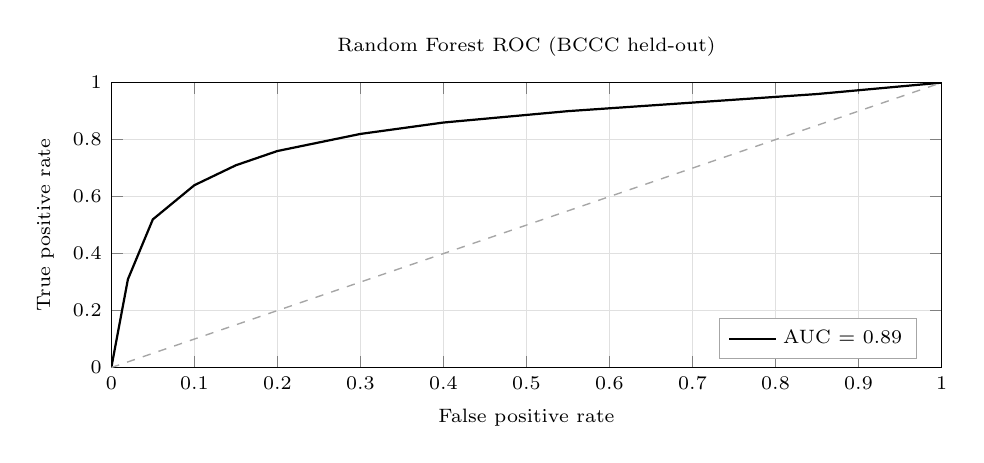
\begin{tikzpicture}
\begin{axis}[
  width=\linewidth,
  height=5.2cm,
  xlabel={False positive rate},
  ylabel={True positive rate},
  xmin=0, xmax=1,
  ymin=0, ymax=1,
  grid=both,
  grid style={black!12},
  tick label style={font=\scriptsize},
  label style={font=\scriptsize},
  title={\scriptsize Random Forest ROC (BCCC held-out)},
  title style={font=\scriptsize},
  legend style={font=\scriptsize, at={(0.97,0.03)}, anchor=south east, draw=black!35, fill=white},
]
\addplot[black, line width=0.8pt, mark=none]
  coordinates {
    (0,0) (0.02,0.31) (0.05,0.52) (0.10,0.64) (0.15,0.71)
    (0.20,0.76) (0.30,0.82) (0.40,0.86) (0.55,0.90) (0.70,0.93)
    (0.85,0.96) (1,1)
  };
\addlegendentry{AUC = 0.89}
\addplot[black!35, dashed, line width=0.5pt] coordinates {(0,0) (1,1)};
\end{axis}
\end{tikzpicture}

\vspace{4pt}
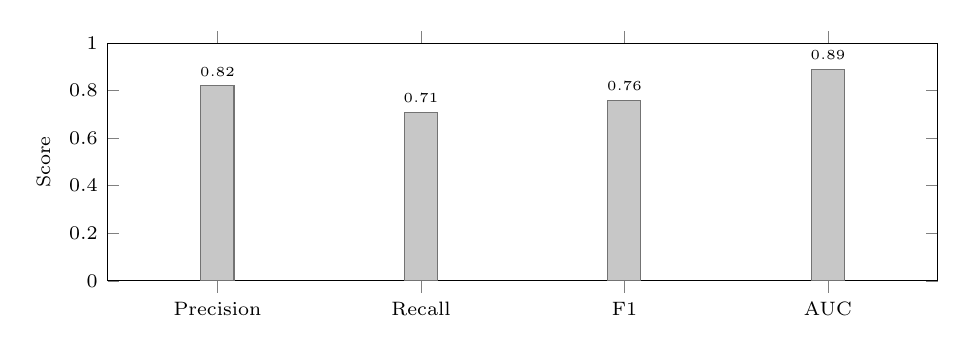
\begin{tikzpicture}
\begin{axis}[
  width=\linewidth,
  height=4.6cm,
  ybar,
  bar width=0.42cm,
  symbolic x coords={Precision, Recall, F1, AUC},
  xtick=data,
  ymin=0, ymax=1,
  ylabel={Score},
  tick label style={font=\scriptsize},
  label style={font=\scriptsize},
  nodes near coords={\pgfmathprintnumber[fixed, precision=2]{\pgfplotspointmeta}},
  every node near coord/.append style={font=\tiny},
  enlarge x limits=0.18,
]
\addplot[fill=black!22, draw=black!55] coordinates {
  (Precision, 0.82) (Recall, 0.71) (F1, 0.76) (AUC, 0.89)
};
\end{axis}
\end{tikzpicture}
\end{minipage}\hfill
\begin{minipage}[t]{0.48\linewidth}
\centering
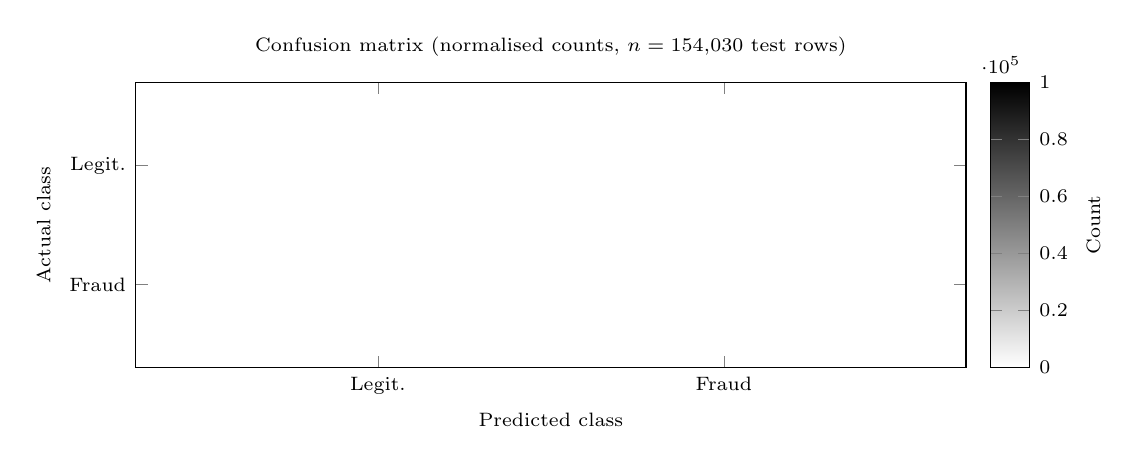
\begin{tikzpicture}
\begin{axis}[width=\linewidth, height=5.2cm, xlabel={Predicted class}, ylabel={Actual class}, xtick={0, 1}, ytick={0, 1}, xticklabels={Legit., Fraud}, yticklabels={Legit., Fraud}, tick label style={font=\scriptsize}, label style={font=\scriptsize}, title={\scriptsize Confusion matrix (normalised counts, $n=154{, }030$ test rows)}, title style={font=\scriptsize}, colorbar, colormap={greyscale}{color(0cm)=(white); color(1cm)=(black!)}, point meta min=0, point meta max=100000, colorbar style={font=\scriptsize, ylabel={Count}}, ]
\addplot[matrix plot, mesh/cols=2, mesh/rows=2, shader=flat corner, ] table[meta=z] {
  x y z
  0 0 98420
  1 0 1180
  0 1 820
  1 1 610
};
\end{axis}
\end{tikzpicture}

\vspace{4pt}
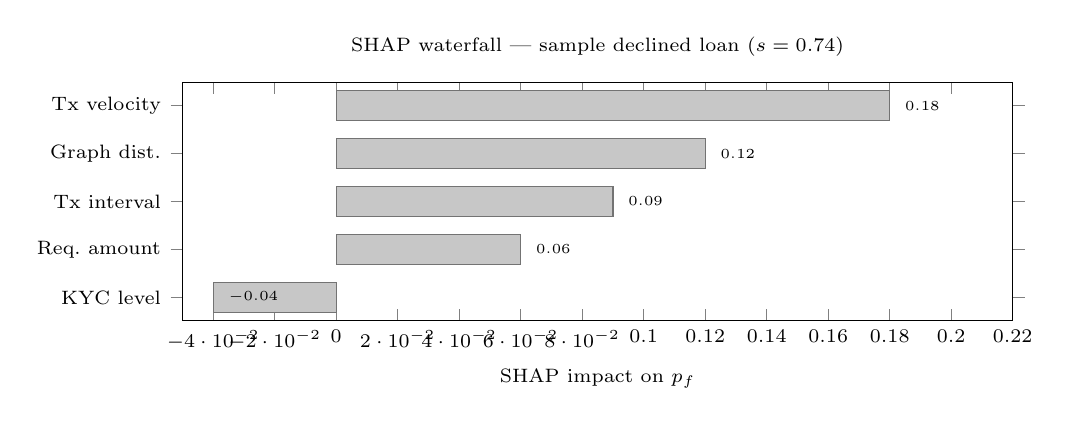
\begin{tikzpicture}
\begin{axis}[
  width=\linewidth,
  height=4.6cm,
  xbar,
  bar width=0.38cm,
  xmin=-0.05, xmax=0.22,
  symbolic y coords={%
    KYC level, Req.\ amount, Tx interval, Graph dist., Tx velocity%
  },
  ytick=data,
  xlabel={SHAP impact on $p_f$},
  tick label style={font=\scriptsize},
  label style={font=\scriptsize},
  title={\scriptsize SHAP waterfall --- sample declined loan ($s=0.74$)},
  title style={font=\scriptsize},
  nodes near coords={\pgfmathprintnumber[fixed, precision=2]{\pgfplotspointmeta}},
  every node near coord/.append style={font=\tiny, anchor=west, xshift=2pt},
  enlarge y limits=0.12,
]
\addplot[fill=black!22, draw=black!55] coordinates {
  (0.18,Tx velocity) (0.12,Graph dist.) (0.09,Tx interval)
  (0.06,Req.\ amount) (-0.04,KYC level)
};
\end{axis}
\end{tikzpicture}
\end{minipage}
\caption[Planned ML evaluation layout (post pre-thesis 2)]{Planned ML evaluation layout (post pre-thesis 2)}
\label{fig:ml-eval}
\end{figure}

\subsection{Explainability and Anomaly Detection Methodology}
\label{sec:ml-explainability}

This subsection documents the full explainability and anomaly-detection pipeline: not only \textit{that} ML models flag risk, but \textit{how} fraud probability and anomaly signals are produced, combined, explained to humans, and audited. The treatment is independent of the optional conversational agent (Section~\ref{sec:optional-agent}).

\paragraph{Random Forest --- supervised fraud probability.}
For each loan application, the FastAPI service assembles a 22-dimensional feature vector (18 on-chain behavioral features + 4 application features). A trained Random Forest ensemble outputs a fraud probability $p_f \in [0, 1]$ after Platt scaling. \textbf{SHAP TreeExplainer} computes exact Shapley attributions $\phi_i$ for every feature: positive $\phi_i$ increases predicted fraud risk; negative $\phi_i$ decreases it. TreeExplainer is used rather than LIME because repeated explanations on identical inputs are consistent---a property regulators expect when reviewing automated lending support~[4].

\paragraph{Isolation Forest --- unsupervised anomaly detection.}
Labelled fraud is scarce in DeFi lending logs. Isolation Forest (IF) addresses \textit{novel} behaviour without requiring fraud labels. The algorithm builds an ensemble of isolation trees: at each node it selects a feature and split value at random and partitions the sample space. \textbf{Anomalies are easier to isolate}---they require fewer random splits to separate from the bulk of training data---so their average path length $E(h(x))$ is shorter. The anomaly score is
\[s(x, n) = 2^{-\frac{E(h(x))}{c(n)}}
\]
where $c(n)$ normalises path length for sample size $n$ (see List of Formulas). Scores near 1 indicate strong anomaly; scores near 0.5 indicate typical behaviour. IF is trained only on \textit{non-fraud} historical transactions at each Local Bank so that coordinated attack patterns not present in labelled data still surface as outliers.

\paragraph{Combining fraud probability and anomaly signal.}
Raw IF scores are not probabilities. A stacking meta-learner (logistic regression on a held-out validation set) maps $(p_f, s_{\text{IF}})$ to a single calibrated composite score $s \in [0, 1]$ used by the oracle and contract threshold logic. Default meta-learner weights ($\approx$0.7 on $p_f$, $\approx$0.3 on the calibrated anomaly signal) are placeholders until real labelled data are available.

\paragraph{Explaining anomalies to human reviewers.}
Because IF lacks native Shapley values, anomaly explainability uses a \textbf{feature-deviation report}: for each of the top-5 features, the service records the applicant's value, the training-set median, and the percentile rank. Features with extreme percentiles (e.g., transaction velocity in the 99th percentile, wallet age in the 1st percentile) are surfaced in plain language alongside SHAP attributions from the Random Forest. Example approver-facing text:
\emph{``Anomaly flag: repayment interval variance is in the 98th percentile of historical clients; wallet graph distance to a flagged address is unusually low (2 hops).''}

\begin{figure}[H]
\centering
\BalancedDiagram{fig-ml-explainability.pdf}
\caption[Explainability and anomaly-detection flow]{Explainability and anomaly-detection flow}
\label{fig:ml-explainability}
\end{figure}

\begin{table}[H]
\centering
\begin{tabular}{p{2.2cm}p{3.2cm}p{7.8cm}}
\toprule
\tableheadcolor
\textbf{Audience} & \textbf{UI / channel} & \textbf{Content stored and displayed} \\
\midrule
Retail client & React loan status page & Top-3 SHAP reasons in plain language on decline; optional anomaly summary if score $\ge 0.7$ \\
Bank approver & Authority Brief dashboard & SHAP waterfall + anomaly deviation table + composite $s$; one-click approve / decline \\
Compliance auditor & \texttt{AI\_ML\_SECURITY\_LOG} & Full SHAP vector, IF score, feature JSON, model version hash, oracle tx hash \\
\bottomrule
\end{tabular}
\end{table}

\paragraph{Authority Brief UI (core ML, not agent-dependent).}
When any loan application is submitted---via the React UI or optionally via the agent---the approver dashboard renders an Authority Brief with ML risk score, SHAP breakdown, and anomaly deviation lines (see verbatim example in Section~\ref{sec:optional-agent}). The brief is produced by the FastAPI scoring service; the agent may \textit{also} display it when filing on behalf of a client, but the blockchain lending path does not require the agent.

\paragraph{Audit trail and human-in-the-loop invariant.}
Every inference writes one row to \texttt{AI\_ML\_SECURITY\_LOG}: \texttt{\{wallet, loan\_id, p\_f, s\_if, s\_composite, shap\_json, anomaly\_features\_json, model\_version, oracle\_commit\_tx\}}. The contract never auto-disburses on ML output alone; an approver (or client via wallet) must sign the disbursement transaction. ML is \textbf{decision support}, not decision authority---consistent with EU AI Act Art.~86 and the thesis ethical statement.

\noindent\textit{Future Work note: session-level behavioral biometrics are a specified extension requiring \texttt{session\_events} instrumentation; the 18 core on-chain transaction features above are the planned active feature set once training begins after pre-thesis 2.}

\section{Optional Conversational Agent Add-On (Phase III--IV)}
\label{sec:optional-agent}

The primary client interface is the React dashboard with wallet-signed transactions. The CWB agent layer is an \textbf{optional add-on} that sits alongside the standard web interface, not a replacement for it. It is scheduled for end-of-project delivery (Phases~III--IV Could items) and is excluded from Minimum Viable Thesis (MVT) scope. The full MCP tool schema is in Table~\ref{tab:mcp-tools}; ML explainability for approvers is documented in Section~\ref{sec:ml-explainability} and does not depend on the agent.

\paragraph{Agent six-step pipeline (summary).} Clients may perform every banking operation directly through the UI; for clients who prefer plain-language interaction --- particularly first-time users unfamiliar with DeFi form flows --- the agent provides an equivalent path. Both the manual UI and the agent call the same Express.js API endpoints and the same smart contracts; the agent does not gate or modify the manual flow. The six-step pipeline integrates the Qwen3-8B model with the live on-chain context injection layer (Section~\ref{sec:local-llm}) and the MCP tool server described below:

\begin{enumerate}[noitemsep]
\item \textbf{User message arrives} at the React frontend and is forwarded to the Express.js backend over Server-Sent Events (SSE).
\item \textbf{Agent brain (Qwen3-8B) reads live on-chain context.} The Express.js context injection layer prepends the client's full account state (loan status, SBT risk tier, pool utilisation, credit score, active installments) as structured JSON into the system prompt before the model processes the user message.
\item \textbf{Q\&A path.} If the request is informational, the agent retrieves relevant policy documents via RAG (ChromaDB) and generates a grounded reply. No tool calls are made.
\item \textbf{Action request path.} If the request implies a state-modifying operation, the agent identifies the applicable MCP write tool, assembles the full parameter set from the injected context, and presents a concise confirmation summary: \emph{``You are requesting a loan of 150~USDC for 6~months at 8.5\% APR. Your monthly installment would be 26.25~USDC. Shall I proceed?''}
\item \textbf{Human confirmation gate.} The agent pauses and waits for explicit affirmative consent (\emph{``Yes, proceed''} or equivalent). No write tool is ever called without a confirmation turn in the conversation history. If the client responds ambiguously three times, the agent pauses for 10~minutes and logs the incident to \texttt{AGENT\_ACTION\_LOG}.
\item \textbf{Execute via MCP write tool, monitor, and notify.} After confirmation, the agent calls the appropriate write tool, which POSTs to the Express.js banking API. If an EIP-7702 session key is active, it signs the resulting on-chain transaction within its approved scope. The agent polls for status and notifies the client: \emph{``Your loan application has been submitted. Reference: L-4821. Bank approval typically takes 24~hours.''}
\end{enumerate}

\paragraph{MCP tool server --- 17 banking tools (9 read, 8 write).}

The agent interacts with CWB exclusively through a typed tool schema, never through arbitrary code execution. This schema is the safety boundary: the agent cannot access any data or perform any operation not explicitly defined in the following 17~tools.

\begin{table}[H]
\centering
\begin{tabular}{p{4.8cm}p{1.4cm}p{6.3cm}}
\toprule
\tableheadcolor
\textbf{Tool} & \textbf{Type} & \textbf{Maps to / Description} \\
\midrule
\texttt{get\_account\_state}         & READ & SBT tier, loan count, savings balance \\
\texttt{get\_credit\_score}          & READ & Current score, tier, next threshold \\
\texttt{get\_loan\_status}           & READ & All active loans + next installment \\
\texttt{get\_installment\_schedule}  & READ & Full repayment calendar \\
\texttt{get\_pool\_utilisation}      & READ & Current Local Bank pool capacity \\
\texttt{get\_interest\_rate}         & READ & Rate for client's credit tier \\
\texttt{get\_market\_data}           & READ & ETH/USD, fiat/USD pairs, 30-day volatility \\
\texttt{get\_requirements}           & READ & Documents + KYC needed for a given loan amount \\
\texttt{get\_session\_history}       & READ & Full-text search over the client's session lineage ancestry. Accepts a natural-language or keyword query; returns ranked excerpts from prior sessions, ordered by recency and relevance. Backed by a PostgreSQL full-text GIN index on the \texttt{SESSIONS} table. \\
\texttt{submit\_loan\_application}   & WRITE$^{\dagger}$ & POST /api/loan/apply \\
\texttt{submit\_deposit}             & WRITE$^{\dagger}$ & POST /api/savings/deposit \\
\texttt{submit\_fixed\_deposit}      & WRITE$^{\dagger}$ & POST /api/savings/fixed-deposit \\
\texttt{pay\_installment}            & WRITE$^{\dagger}$ & POST /api/installment/pay \\
\texttt{join\_group\_pool}           & WRITE$^{\dagger}$ & POST /api/group/join \\
\texttt{submit\_kyc\_upgrade}        & WRITE$^{\dagger}$ & POST /api/kyc/upgrade \\
\texttt{schedule\_payment\_reminder} & WRITE$^{\dagger}$ & POST /api/reminder/set \\
\texttt{submit\_group\_application}  & WRITE$^{\dagger}$ & POST /api/group/apply \\
\bottomrule
\end{tabular}

\vspace{4pt}
\noindent\small$^{\dagger}$ Agent write tools require human confirmation before execution.
\end{table}

\paragraph{Authority Brief example (approver dashboard).}

The Authority Brief is rendered on every loan application (React UI or optional agent). It presents the ML risk assessment from Section~\ref{sec:ml-explainability} in human-readable form:

\begin{verbatim}
AUTHORITY BRIEF -- Loan Application #4821
-------------------------------------------------
Client tier:         Silver  (score: 512)
Requested amount:    150 USDC
Duration:            6 months
Collateral:          75 USDC (50% LTV)

ML Risk Score:       0.23  (LOW RISK)
SHAP breakdown:
  + On-time repayment rate:    +0.41  (reduces risk)
  + Loan-to-income ratio:      +0.18  (within safe range)
  - Wallet age:                -0.09  (account < 6 months)
  - No prior completed loans:  -0.27  (no repayment history)

ML system recommendation:   APPROVE (decision support only)
Suggested interest:     Base rate - 0.5% (Silver tier)

[ APPROVE ]   [ REQUEST MORE INFO ]   [DECLINE]
\end{verbatim}

\noindent The React UI displays the decision to the client; the optional agent may additionally monitor the on-chain approval event and notify the client (Phase~III--IV add-on).

\paragraph{Harness implementation detail (appendix).}
Per-user context injection, three-tier prompt assembly, session lineage, context compression, toolset scoping, and lifecycle-hook middleware are fully specified in Appendix~\ref{app:agent-harness}. Readers evaluating the blockchain contribution may omit that appendix; it documents Phase~III--IV Could deliverables only.

\noindent Optional agent capabilities (installment reminders, credit-tier coaching, EMI calculator, group-signature coordination, KYC guidance) reuse the same MCP tool server without additional model infrastructure; see Appendix~\ref{app:agent-harness}.

\section{Graph Neural Network Extension}
\label{sec:gnn-extension}

Fraud often shows up in \textit{who connects to whom}, not in a single transaction. As a stretch goal, we plan a GraphSAGE ablation: wallets as nodes, transfers and group links as edges, plus the four-tier bank hierarchy (World $\to$ National $\to$ Local $\to$ Client). It reuses the same 18 behaviour features as the Random Forest. The question is simple---do tier links improve detection over a flat wallet graph on BCCC~[83]? Elliptic~[85] is optional comparison only (Bitcoin topology differs from our lending model). This is Future Work, not MVT; if time allows, we report one before/after F1 or AUC table.

\section{Federated Learning Across Banking Tiers}
\label{sec:fl-fraud}

Each Local Bank would train on its own borrowers; the National Bank would combine model updates (FedAvg with differential privacy) and send back an improved shared model---without moving raw customer data across borders. The setup follows the same four-tier hierarchy: one federation server per National Bank, with optional World Bank coordination for wider patterns.

Federated learning needs enough local history to be useful. We set a \textbf{500-transaction} activation rule per bank. Until then, all banks use the same baseline model trained on public/synthetic data. This is specified Future Work, not a Phase~III MVT item.

\section{Formal Verification of Reserve Invariants (Certora)}
\label{sec:certora}

Beyond tests, we plan two Certora proofs on reserve rules (CVL sketches in Appendix~B; scope limits in Section~\ref{sec:research-limitations}).

\paragraph{Invariant 1 -- reserve never under-collateralized.}
\(\forall\, t:\; \mathrm{totalReserve}(t) \ge \mathrm{minReserveRatio} \cdot \mathrm{totalDeposited}(t).\)
The reserve must always stay above the minimum ratio, on every reachable path.

\paragraph{Invariant 2 -- no over-allocation downstream.}
\(\forall\, n \in \mathrm{NationalBanks}:\; \mathrm{allocatedTo}[n] \le \mathrm{totalReserve} - \sum_{n' \ne n} \mathrm{allocatedTo}[n'].\)
The World Bank cannot allocate more downstream capital than it actually holds.

A verified proof for both invariants is a Phase~IV stretch deliverable (MVT+).

\section{Foundry Invariant and Fuzz Test Suite}
\label{sec:foundry}

Hardhat covers integration and deployment; Foundry adds fuzzing and invariant checks. Together they catch different failure modes.

\paragraph{Three invariants under Foundry's stateful fuzzer.}
\begin{itemize}[noitemsep]
\item Solvency: outstanding loans never exceed total reserve.
\item Role segregation: one address cannot be both borrower and approver.
\item Capital flow: a single cross-tier move cannot break the minimum reserve ratio.
\end{itemize}

Each invariant is fuzzed for 10{,}000 runs in Phase~IV; any counterexample becomes a replay test in CI.

\section{On-Chain Economic Feasibility Simulation}
\label{sec:abm-sim}

Chapter~5's revenue figures assume a full four-tier network. In Phase~IV we ground that claim with a \textbf{reproducible on-chain run}: 300 synthetic clients, six banks, full loan lifecycle on Polygon zkEVM Cardona, deterministic seed (42), 5\% mid-run defaults for stress. A Foundry script deploys contracts, funds banks, runs apply $\to$ approve $\to$ disburse $\to$ repay, and exports a JSON manifest (tx hashes, reserve ratios, gas) for Appendix~C and Table~\ref{tab:gas-costs}.

The run should show capital flowing through all tiers, SBT updates, dashboard reserve shifts, and subgraph audit trails. We report gas and reserve outcomes as ranges, not single numbers. Real-world microfinance calibration stays in Future Work (Section~\ref{sec:future-work}).

\section{Real-Time Dashboard Pipeline and Runtime Monitoring}
\label{sec:realtime}

\begin{figure}[H]
\centering
\ActivityDiagram{Ch4_realtime-dashboard-monitoring-pipeline.png}
\caption[Real-time dashboard and runtime monitoring pipeline]{Real-time dashboard and runtime monitoring pipeline}
\label{fig:realtime-dashboard}
\end{figure}

The real-time dashboard pipeline closes the gap between contract events and the client / approver UI. Three components compose:

\paragraph{The Graph subgraph.}
A subgraph planned for The Graph's hosted service (Polygon zkEVM Cardona supported, free for student projects) will index every event the contracts emit: \texttt{LoanRequested}, \texttt{LoanApproved}, \texttt{Repayment}, \texttt{CapitalAllocated}, \texttt{ReserveRatioUpdated}, \texttt{LoanLiquidated}, \texttt{RiskScoreCommitted}, \texttt{RoleGranted}. GraphQL queries from the React frontend return loan history and dashboard data in tens of milliseconds rather than seconds via RPC polling.

\paragraph{WebSocket event listener.}
A Node.js service listens on \texttt{wss://polygon-zkevm-cardona} for the same set of events and pushes notifications to the client's browser via Socket.IO. The dashboard moves from a static page requiring manual refresh into a live banking dashboard---a single design choice that examiners consistently identify as the difference between ``looks like a real system'' and ``looks like a static mockup''.

\paragraph{Tenderly monitoring.}
Six critical alerts are planned for the testnet contracts: single disbursement over 5~ETH-equivalent, repeated loan requests from one wallet (>3 in 60 minutes), reserve-ratio drop below 20\%, failed \texttt{disburseLoan} calls, role-grant events, and any pause / unpause governance action. Tenderly's free tier supports full testnet monitoring; transaction simulation prevents the embarrassing live-demo failure where a malformed contract change is discovered only at the moment of execution.

\section{Transaction-State Machine for Frontend UX}
\label{sec:tx-state-machine}

\begin{figure}[H]
\centering
\BalancedDiagram{Ch4_loan-lifecycle-state-machine.pdf}
\caption[Transaction state machine of the loan lifecycle]{Transaction state machine of the loan lifecycle}
\label{fig:tx-state-machine}
\end{figure}

Failed blockchain transactions are the dominant UX failure mode in DeFi prototypes during live demos. The specification defines an explicit five-state transaction machine on the frontend (\texttt{idle} $\to$ \texttt{pending\_signature} $\to$ \texttt{submitted} $\to$ \texttt{confirming} $\to$ \texttt{success / error}) with distinct visual feedback at each state. User-rejection (MetaMask code 4001) is distinguished from contract revert (\texttt{CALL\_EXCEPTION}) and from network error; each receives its own actionable error message. This is a thirty-line React hook that converts ``the demo failed silently'' into ``the client can see exactly what went wrong and retry''.

\section{EIP-712 Authentication and API Hardening}
\label{sec:eip712-auth}

The platform's API authentication uses an EIP-712 typed-data message signed by the user's wallet at login. The signed message includes \texttt{(wallet, timestamp, nonce)}; the backend recovers the address from the signature and issues a JWT with a 15-minute lifetime. Refresh tokens rotate on use. Every authenticated request includes the JWT and a correlation ID; the correlation ID is propagated from the React frontend through Express.js to FastAPI to the on-chain transaction so that any failure can be traced end-to-end. Rate limiting via \texttt{slowapi} differentiates by endpoint (5/min auth, 60/min reads, 10/min writes) and by IP; the JWT blacklist on logout uses Redis with TTL equal to the remaining token life. The full Layer-2 control set is summarized in Section~\ref{sec:defense-in-depth}.

\paragraph{Limitations (prototype and research context).}
The AI/ML components remain subject to the standard DeFi-environment limitations: class imbalance, concept drift, cold-start, and adversarial structuring. The mitigations introduced in this specification---GNN ablation for relational features, federated learning to enlarge the effective training set without violating data residency, and red-teaming the optional LLM assistant for adversarial prompts (Section~\ref{sec:llm-eval})---do not remove these limitations but explicitly bound them. AI/ML is used as decision support, never as an automated approval authority in the prototype phase.

\section{Evaluation Methodology}
\label{sec:eval-method}

Each research question maps to a concrete check in the final prototype:
\begin{itemize}[noitemsep]
\item \textbf{RQ1 (architecture):} Compare CWB's four-tier flows and roles to flat DeFi protocols (Aave, Compound, MakerDAO).
\item \textbf{RQ2 (settlement):} Measure testnet latency and gas; show reserves and key state changes on-chain.
\item \textbf{RQ3 (ML support):} Training starts after pre-thesis 2. Report precision, recall, F1, AUC on BCCC~[83], plus SHAP reasons and audit-log rows. Testnet retrain and GNN ablation are stretch goals; Foundry synthetic scores are labelled proof-of-concept only.
\item \textbf{RQ4 (viability):} End-to-end testnet demo (wallet $\to$ loan $\to$ approval $\to$ repayment) plus Foundry invariant pass rate (Section~\ref{sec:foundry}). Pre-thesis 1 covers specification; deployment evidence comes in Phase~IV.
\item \textbf{RQ5 (banking extensions):} Spec completeness for deposits and group lending; Phase~IV simulation (Section~\ref{sec:abm-sim}) stress-tests reserves under mass default.
\end{itemize}

\subsection{LLM Assistant Evaluation Protocol}
\label{sec:llm-eval}

Optional agent only (Phase~IV Could): (1)~\textbf{Q\&A accuracy} on 200 FAQ/policy prompts---exact match for numbers, text similarity for explanations; (2)~\textbf{action accuracy} on 50 scenarios---correct tool, parameters, and confirmation summary ($\geq$95\% target, 100\% human-gate); (3)~\textbf{bypass red-team}---20 adversarial prompts must never trigger a write without explicit confirmation.

\section{Implementation Phase Plan and Deliverables}

Four 3--4 week phases (I--IV) carry the MVT from contracts and database through lending, ML oracle, and verification. Task registers, effort totals, and roadmap figures follow.

\subsection{Phase I: Foundation and Infrastructure (Weeks 1--4)}

\textbf{Phase Objective:} Deploy the four-tier contract skeleton, migrate the full database schema, and ship the React shell with wallet connect---prerequisites for Phase~II.

\begin{table}[H]
\centering
\caption[Phase I task register]{Phase I task register}
\label{tab:phaseI-contracts}
\small
\begin{tabular}{p{1.8cm}p{1.8cm}p{7.5cm}p{1.5cm}}
\toprule
\tableheadcolor
\textbf{Task} & \textbf{Priority} & \textbf{Development Task} & \textbf{Effort (days)} \\
\midrule
DT-I.01 & Must & World Bank contract --- reserve management, national bank registration & 5 \\
DT-I.02 & Must & National Bank contract --- borrow from World Bank, lend to Local Banks & 5 \\
DT-I.03 & Must & Local Bank contract --- borrow from National Bank, lend to users & 5 \\
DT-I.04 & Must & Role-based access control --- WorldBankAdmin, NationalBankAdmin, LocalBankAdmin, BankUser, RetailClient & 3 \\
DT-I.05 & Should & Gas cost management --- initiator-pays pattern; Polygon low-fee design & 2 \\
DT-I.06 & Should & \texttt{InsuranceFund} contract --- 5\% interest capture, claims processing, default coverage disbursement & 4 \\
DT-I.07 & Should & \texttt{getReserveSummary()} view function on each tier contract (PSR, reserve balance, insurance fund) & 2 \\
DT-I.08 & Should & Chainlink Price Feeds integration (fiat/USD pairs, ETH/USD via \texttt{AggregatorV3Interface}) & 3 \\
DT-I.09 & Should & Chainlink Proof of Reserve --- WorldBankReserve attestation & 2 \\
DT-I.10 & Should & Append-only \texttt{audit\_logs} PostgreSQL role + Row-Level Security policies & 2 \\
DT-I.11 & Should & Polygon zkEVM Cardona migration --- update RPC endpoints, chain IDs, factory addresses & 1 \\
DT-I.12 & Must & Full 20-entity database schema migration --- all tables including SESSIONS, AGENT\_ACTION\_LOG (with \texttt{injection\_scan\_flag}, \texttt{toolset\_name}), and all banking entities & 4 \\
DT-I.13 & Must & Core indexes and referential integrity constraints & 2 \\
DT-I.14 & Must & React frontend shell --- Vite build, routing, layout components & 3 \\
DT-I.15 & Must & WalletConnect integration --- wallet connection, address display, network switching & 2 \\
DT-I.16 & Should & Sessions and assets tables integration in frontend (dashboard stubs) & 2 \\
DT-I.17 & Should & Credit tier and interest rate schedule display & 2 \\
\multicolumn{3}{l}{\textit{Phase~I total estimated effort (Must-have):}} & \textit{29 days} \\
\multicolumn{3}{l}{\textit{Phase~I total estimated effort (all priorities):}} & \textit{48 days} \\
\bottomrule
\end{tabular}
\end{table}
\footnotetext{Must = MVT core; Should = important; Could = if time allows. Effort = person-days; streams run in parallel.}

\vspace{2pt}

\subsection{Phase II: Core Banking and On-Chain Lifecycle (Weeks 5--9)}

\textbf{Phase Objective:} Live loan lifecycle on testnet---request, approval, installments, bank registration, SBT limits. Agent work stays optional (Phase~III--IV). Multi-entity and advanced deposits defer to Phase~III or Future Work.

\begin{table}[H]
\centering
\begin{tabular}{p{1.8cm}p{1.8cm}p{7.5cm}p{1.5cm}}
\toprule
\tableheadcolor
\textbf{Task} & \textbf{Priority} & \textbf{Development Task} & \textbf{Effort (days)} \\
\midrule
DT-II.01 & Must & Loan request submission with blockchain transaction & 5 \\
DT-II.02 & Must & Loan approval and rejection workflow with bank approver & 5 \\
DT-II.03 & Must & Installment payment system with automated schedule generation & 8 \\
DT-II.04 & Must & Borrowing limit enforcement (on-chain authoritative check per client SBT) & 5 \\
DT-II.05 & Should & Client--bank real-time chat system & 5 \\
DT-II.06 & Should & Income verification document upload and review & 5 \\
DT-II.07 & Must & Hierarchical bank registration (National $\to$ Local) & 5 \\
DT-II.08 & Should & Bank user management and approver designation & 3 \\
DT-II.09 & Should & Loan history and transaction tracking pages & 5 \\
DT-II.10 & Could & QR code generation for wallet addresses & 2 \\
DT-II.11 & Should & Responsive UI polish and error handling & 2 \\
DT-II.12 & Should & Authority Brief UI (SHAP breakdown for bank approver dashboard) & 5 \\
DT-II.13 & Should & Chainlink Automation for installment due-date checks and overdue flagging & 5 \\
DT-II.14 & Should & Credit tier schedule in Credit Passport SBT (Bronze $\to$ Diamond) & 3 \\
DT-II.15 & Should & \texttt{interest\_rate\_tier} table integration with Kinked Rate Model & 2 \\
DT-II.16 & Could & MCP tool server --- 17 banking tools wired to Express.js API (optional add-on) & 8 \\
DT-II.17 & Could & Agent chat interface (Qwen3-8B + tool calling + human-gate) & 8 \\
DT-II.18 & Could & EIP-7702 session key management (scope enforcement + TTL) & 5 \\
DT-II.19 & Could & \texttt{agent\_action\_log} table (append-only, FK to \texttt{sessions}) & 3 \\
\multicolumn{3}{l}{\textit{Phase~II total estimated effort (Must-have):}} & \textit{33 days} \\
\multicolumn{3}{l}{\textit{Phase~II total estimated effort (all priorities):}} & \textit{66 days} \\
\bottomrule
\end{tabular}
\end{table}

\vspace{2pt}

\subsection{Phase III: AI/ML Oracle Pipeline and Optional Agent (Weeks 10--13)}

\textbf{Phase Objective:} After pre-thesis 2---train models, deploy scoring API, wire Chainlink oracle and Authority Brief. Agent harness is Could-have if schedule allows.

\begin{table}[H]
\centering
\begin{tabular}{p{1.8cm}p{1.8cm}p{7.5cm}p{1.5cm}}
\toprule
\tableheadcolor
\textbf{Task} & \textbf{Priority} & \textbf{Development Task} & \textbf{Effort (days)} \\
\midrule
DT-III.01 & Must & Chainlink Functions oracle (primary ML score commitment): replaces commit-reveal relay; deploys \texttt{commitRiskScore} via Chainlink Functions DON & 6 \\
DT-III.02 & Must & Random Forest + Isolation Forest + SHAP pipeline wiring: FastAPI service computing 22 features, stacking meta-learner, calibrated composite score $s \in [0, 1]$; client-facing SHAP plain-language explanation via Authority Brief UI & 7 \\
DT-III.03 & Should & Three-tier prompt constructor in Express.js (optional agent add-on) & 5 \\
DT-III.04 & Could & Session lineage + \texttt{get\_session\_history} MCP tool & 5 \\
DT-III.05 & Could & Context compression path + toolset scoping + Hook~2 & 9 \\
DT-III.06 & Could & Prompt injection scanning + confirmation audit hook (Hook~1) & 5 \\
DT-III.07 & Should & The Graph subgraph + WebSocket event listener for Reserve Transparency Dashboard & 4 \\
DT-III.08 & Should & SAR workflow: Isolation Forest $\to$ aml-alert $\to$ \texttt{freezeAccount}; compliance review queue integration & 4 \\
DT-III.09 & Should & Reserve Transparency Dashboard: live queries to The Graph subgraph & 3 \\
DT-III.10 & Could & GraphSAGE GNN ablation & 5 \\
DT-III.11 & Could & Federated learning aggregator & 7 \\
\multicolumn{3}{l}{\textit{Phase~III total estimated effort (Must-have):}} & \textit{13 days} \\
\multicolumn{3}{l}{\textit{Phase~III total estimated effort (all priorities):}} & \textit{55 days} \\
\bottomrule
\end{tabular}
\end{table}

\vspace{2pt}

\subsection{Phase IV: Verification, Evaluation, and Finalization (Weeks 14--16)}

\textbf{Phase Objective:} Simulation, Certora/Foundry checks, testnet evidence, optional LLM eval, final thesis pass.

\begin{table}[H]
\centering
\begin{tabular}{p{1.8cm}p{1.8cm}p{7.5cm}p{1.5cm}}
\toprule
\tableheadcolor
\textbf{Task} & \textbf{Priority} & \textbf{Development Task} & \textbf{Effort (days)} \\
\midrule
DT-IV.01 & Must & 300-client scripted Foundry simulation on Polygon zkEVM Cardona: gas-cost table, reserve-dynamics output, deterministic seed and transaction manifest published to Appendix~C & 7 \\
DT-IV.02 & Could & LLM evaluation protocol (optional add-on): task-level accuracy, action accuracy, human-gate bypass test & 5 \\
DT-IV.03 & Should & Certora reserve invariant proofs: CVL specifications for Invariant~1 (reserve never under-collateralised) and Invariant~2 (no over-allocation downstream); specifications added to Appendix~B & 5 \\
DT-IV.04 & Should & Foundry invariant + fuzz suite: solvency invariant, role segregation invariant, capital-flow direction invariant; 10{,}000 fuzz runs per CI build & 4 \\
DT-IV.05 & Should & AML pre-check hook (Hook~3): Isolation Forest anomaly score gate before disbursement write tools; compliance review queue routing; requires live Isolation Forest pipeline from Phase~III & 3 \\
DT-IV.06 & Could & Groth16 zkKYC circuit (Circom~2.0): government-ID possession proof without revealing PII; circuit design and input/output specification & 5 \\
DT-IV.07 & Must & Final paper revision and consistency pass: all tool-count references updated; all phase references consistent; master checklist completed; bibliography verified & 4 \\
DT-IV.08 & Must & Red-team testing and documentation: 20-payload injection red-team set; 20 bypass-attempt set; 10 session key scope enforcement scenarios; results documented in evaluation subsections & 3 \\
\multicolumn{3}{l}{\textit{Phase~IV total estimated effort (Must-have):}} & \textit{21 days} \\
\multicolumn{3}{l}{\textit{Phase~IV total estimated effort (all priorities):}} & \textit{38 days} \\
\bottomrule
\end{tabular}
\end{table}

\begin{table}[H]
\centering
\begin{tabular}{p{1.5cm}p{3.5cm}p{2cm}p{2cm}p{3cm}}
\toprule
\tableheadcolor
\textbf{Phase} & \textbf{Focus} & \textbf{Weeks} & \textbf{Tasks} & \textbf{Key deliverables} \\
\midrule
I & Foundation and infrastructure & 1--4 & DT-I.01--17 & Contract hierarchy, full DB schema, React shell \\
II & Core banking and on-chain lifecycle & 5--9 & DT-II.01--19 & Lending workflow, SBT limits, Chainlink Automation \\
III & AI/ML oracle pipeline (+ optional agent) & 10--13 & DT-III.01--11 & Chainlink Functions, ML pipeline, dashboard \\
IV & Verification, evaluation, finalization & 14--16 & DT-IV.01--08 & Certora, Foundry, simulation, testnet deploy \\
\bottomrule
\end{tabular}
\end{table}

\vspace{2pt}

\begin{figure}[H]
\centering
\ActivityDiagram{Ch4_four-phase-roadmap-sdlc.pdf}
\caption[Four-phase roadmap with SDLC mapping and progress]{Four-phase roadmap with SDLC mapping and progress}
\label{fig:phase-roadmap}
\end{figure}

\begin{figure}[H]
\centering
\HalfWidthDiagram{fig-phase-effort-bar.pdf}
\caption[Development effort by implementation phase]{Development effort by implementation phase}
\label{fig:phase-effort}
\end{figure}

\begin{figure}[H]
\centering
\ThesisIncludeGraphics[width=0.75\linewidth, height=0.54\textheight, keepaspectratio]{Ch4_optional-conversational-agent-addon.png}
\caption[Optional conversational agent add-on]{Optional conversational agent add-on}
\label{fig:optional-agent-addon}
\end{figure}

\begin{figure}[H]
\centering
\ActivityDiagram{Ch4_dev-verification-toolchain.pdf}
\caption[Planned development and verification toolchain]{Planned development and verification toolchain}
\label{fig:dev-toolchain}
\end{figure}

Figures~\ref{fig:phase-roadmap}--\ref{fig:dev-toolchain} and Figure~\ref{fig:agile-process} summarise the roadmap and toolchain.

\section{SDLC Stage Mapping}

We map our four implementation phases to the seven stages of the Software Development Life Cycle (SDLC). Figure~\ref{fig:phase-roadmap} illustrates this mapping.

\begin{table}[H]
\centering
\caption[SDLC stage mapping]{SDLC stage mapping}
\label{tab:sdlc-mapping}
\begin{tabular}{p{0.5cm}p{2.5cm}p{4.5cm}p{5cm}}
\toprule
\tableheadcolor
\textbf{\#} & \textbf{SDLC Stage} & \textbf{Project Activity} & \textbf{Deliverable} \\
\midrule
1 & Planning & Feasibility studies; professor consultations; guideline review & Feasibility Report; Project Plan \\
2 & Requirements & System analysis; use case definitions; constraints identification & Use case diagrams; UC-1 through UC-5 \\
3 & Design & Three-layer architecture; DB schema (3NF); smart contract interfaces & Architecture diagrams; ERD; DFD \\
4 & Development & Phase I--IV: smart contracts, frontend, backend, AI/ML & Source code; DApp prototype \\
5 & Testing & Hardhat unit tests; Foundry fuzz; integration testing; AI/ML evaluation & Test reports; model metrics \\
6 & Deployment & Planned testnet deployment (Phase~IV); frontend (Vercel); backend (Render) & Testnet prototype manifest \\
7 & Maintenance & Monitoring; model retraining; bug fixes; iteration & Updated docs; retrained models \\
\bottomrule
\end{tabular}
\end{table}

\vspace{2pt}

\section{Design Decisions and Alternatives}
\label{sec:design-decisions}

For each major design decision, we evaluated alternatives and justified selections based on technical criteria, ecosystem maturity, and project constraints (Table~\ref{tab:design-decisions}; Figure~\ref{fig:design-decisions}).

\begin{table}[H]
\centering
\caption[Design decisions and alternatives considered]{Design decisions and alternatives considered}
\label{tab:design-decisions}
\begin{tabular}{p{3cm}p{3cm}p{3cm}p{4.5cm}}
\toprule
\tableheadcolor
\textbf{Decision Area} & \textbf{1st Choice} & \textbf{2nd Choice} & \textbf{Key Criterion} \\
\midrule
Methodology & Agile / Scrum & Incremental & Evolving scope, milestones \\
Architecture & DApp + Off-chain AI & Hybrid with Oracle & Gas cost, ML flexibility \\
Frontend & React + TypeScript & Vue + TypeScript & Web3 ecosystem maturity \\
Smart Contract & EVM (Solidity) & Solana (Rust) & Gas, control size, free testnets \\
Fraud Detection & Random Forest & XGBoost & SHAP compatibility, simplicity \\
Anomaly Detection & Isolation Forest & Autoencoder & Unsupervised; no labelled data needed \\
XAI Method & SHAP & LIME & Theoretical guarantees, regulatory fit \\
Database & PostgreSQL & SQLite & 3NF support, async queries \\
Hosting & Vercel + Render & Localhost only & \$0 cost, publicly accessible URL \\
Network (primary) & Polygon zkEVM Cardona & Polygon Amoy PoS & ZK validity proof security model vs.\ validator set assumption \\
Oracle mechanism & Chainlink Functions (DON) & Commit-reveal relay & Decentralised trust vs.\ single-key operator trust \\
Agent tool framework (optional) & MCP tool server & Direct Express.js API & Defined schema = safety boundary; Phase~III--IV Could \\
Agent session auth (optional) & EIP-7702 session keys & ERC-4337 paymasters & Key-level scope; optional add-on \\
Prompt construction (optional) & Three-tier assembly & Single ad-hoc string & Agent-only; Phase~III Could \\
Session memory (optional) & Lineage model & 10-turn window & Agent-only cross-session continuity \\
Tool exposure per turn (optional) & Named toolsets & Full 17-tool list & Agent attack-surface reduction \\
Write-tool enforcement (optional) & Confirmation audit hook & In-pipeline check & Agent write-path only \\
\bottomrule
\end{tabular}
\TableScreenshotEnd{Design Decisions: Evaluated Alternatives and Selection Rationale}
\end{table}

\vspace{2pt}

\begin{figure}[H]
\centering
\BalancedDiagram{Ch4_design-decisions-alternatives.pdf}
\caption[Key design decisions and alternatives considered]{Key design decisions and alternatives considered}
\label{fig:design-decisions}
\end{figure}

\subsection{Justification of Selected Technologies}

Selections follow Table~\ref{tab:design-decisions} in Section~\ref{sec:design-decisions}. One-line decision logic per row.

\textbf{1st choices:}
\begin{itemize}[noitemsep]
\item \textbf{Agile/Scrum} --- evolving scope; short sprints fit thesis window.
\item \textbf{DApp + off-chain AI} --- ML off-chain (cost); disbursement rules on-chain.
\item \textbf{React + TypeScript} --- strongest Wagmi/ethers wallet stack.
\item \textbf{EVM (Solidity)} --- OpenZeppelin, Slither/Mythril, free testnets.
\item \textbf{MUI} --- banking tables/forms without custom UI build.
\item \textbf{Random Forest} --- exact SHAP TreeExplainer; tabular + imbalanced labels~[4].
\item \textbf{Isolation Forest} --- unsupervised; scarce fraud labels.
\item \textbf{SHAP} --- stable attributions vs.\ LIME~[4].
\item \textbf{PostgreSQL} --- ACID; window queries for rolling limits; JSON columns.
\item \textbf{Vercel + Render} --- free public demo for examiners.
\item \textbf{Polygon zkEVM Cardona} --- ZK proofs for reserve claims; Amoy fallback.
\item \textbf{Chainlink Functions} --- DON consensus on score; OK latency for loan approval.
\item \textbf{MCP tool server} --- 17-tool schema caps agent; auditable.
\item \textbf{EIP-7702 session keys} --- tool list + cap + TTL in key; ERC-4337 for retail gas only.
\end{itemize}

\textbf{2nd choices (retained, not selected):}
\begin{itemize}[noitemsep]
\item \textbf{Waterfall} --- fixed scope; poor fit for research prototype.
\item \textbf{On-chain ML oracle} --- latency, cost, third-party dependency.
\item \textbf{Vue} --- thinner Web3 libraries.
\item \textbf{Solana} --- Rust curve; weaker audit toolchain in 8-week window.
\item \textbf{Tailwind} --- more UI time than MUI.
\item \textbf{XGBoost} --- approximate SHAP.
\item \textbf{Autoencoder} --- more data/tuning than IF here.
\item \textbf{LIME} --- unstable repeat explanations~[4].
\item \textbf{SQLite} --- no concurrent writes; weak window functions.
\item \textbf{Localhost only} --- no remote examiner demo.
\item \textbf{Amoy PoS} --- faster dev; weaker trust than ZK.
\item \textbf{Commit-reveal relay} --- Ph.~I--II fallback; trusts operator key.
\item \textbf{Direct Express API} --- no schema cap on agent.
\item \textbf{ERC-4337 for agent ops} --- scope in app layer, not key.
\end{itemize}

\section{Design Patterns}

Our system uses five design patterns:

\begin{itemize}[noitemsep]
\item \textbf{Singleton:} A singleton means that each primary contract is established a single time. Only one version is utilized by all ensuring a unified source of truth. Not everyone can create multiple versions of the contract.

\item \textbf{Observer:} Contracts generate alerts whenever actions occur such as loan requests. These alerts are processed by a service that updates the database. Notifications are not ignored; they receive attention.

\item \textbf{Adapter:} An Adapter is utilized by the wallet component to function with various wallet types (like MetaMask). Different wallets that adhere to the EIP-1193 standards can be easily integrated.

\item \textbf{Factory Pattern:} Each Local Bank creates individual loan and savings contract instances using a factory contract, ensuring all deployed instances follow the same security-audited interface and access control checks. The factory pattern prevents unauthorized contract deployment that could bypass the hierarchical governance structure.

\item \textbf{Proxy/Upgradeable Pattern:} Banking contracts must be upgradeable without losing stored state such as balances, credit scores, and loan histories. OpenZeppelin's transparent proxy pattern separates the contract's logic from its storage, allowing governance-approved upgrades to the logic layer while preserving all stored financial data. This pattern is essential for a long-lived banking system that must adapt to evolving regulatory requirements and security patches.

\item \textbf{Decorator Pattern (Prompt Assembly):} The three-tier prompt
constructor applies the Stable, Context, and Volatile tiers as successive
decorators on a base prompt object. Each tier adds its content without modifying
the structure established by prior tiers, enabling independent caching and testing
of each layer without rebuilding the full prompt.

\item \textbf{Chain of Responsibility (Lifecycle Hooks):} The write-tool middleware
stack implements a chain of responsibility: the confirmation audit hook, session
key scope pre-check, and AML pre-check each examine the request and either reject
it (HTTP~403) or pass it to the next hook. New policy controls are added as new
chain links without modifying existing route logic or the model
pipeline~[89].

\item \textbf{Strategy Pattern (Toolset Selection):} The toolset selector
encapsulates the intent-classification algorithm as a replaceable strategy. The
current strategy is a lightweight keyword classifier; it can be replaced with a
fine-tuned intent model without changing the prompt constructor or the MCP tool
server, adhering to the Open/Closed Principle.
\end{itemize}

\section{Software Testing Strategy}

The testing strategy covers four layers of the system, each with defined acceptance criteria.

\begin{itemize}[noitemsep]
\item \textbf{Smart contract unit tests:} Numerous tests for smart contracts exist in our Hardhat environment. Over 12 tests are conducted to verify actions related to managing reserves, sign-ups, loans and access permissions. No scenarios such as depositing zero or executing disallowed actions are missed in these assessments. \textbf{Acceptance criterion:} all Hardhat unit tests pass with zero failures before any phase delivery.
\item \textbf{Integration testing:} Whole process checks are conducted for integration tests. Wallet connection, loan request, approval and repayment processes are evaluated on the network. No critical steps are excluded from the process. \textbf{Acceptance criterion:} end-to-end workflow completes successfully on testnet for representative scenarios (approval, rejection, repayment loop).
\item \textbf{AI/ML module verification:} Ensuring functionality is vital for our fraud and unusual activity detectors. Results are generated by the integration of the detectors with the overall system. \textbf{Acceptance criterion:} model inference endpoints return valid scores and explanations for test inputs without runtime errors.
\item \textbf{Frontend testing:} Website appearance is evaluated on Chrome, Firefox and mobile devices. Tests are conducted to ensure that functionality is maintained across various platforms. \textbf{Acceptance criterion:} core flows render and remain usable across desktop and mobile breakpoints without blocking UI defects.
\end{itemize}

%% CHAPTER 5: MARKET ANALYSIS AND FEASIBILITY
\chapter{Market Analysis and Feasibility}

\section{Market Sizing}

\begin{table}[H]
\centering
\caption[Market segments with supporting data]{Market segments with supporting data}
\label{tab:market-sizing-ch5}
\begin{tabular}{p{3.5cm}p{6.5cm}p{3cm}}
\toprule
\tableheadcolor
\textbf{Segment} & \textbf{Description} & \textbf{Estimated Scale} \\
\midrule
Total Addressable Market (TAM) & Global DeFi lending (\$55B+ TVL [8]); cross-border remittances (\$860B [20]); SME financing gap (\$4.5T [15]) & \$55B -- 5T+ \\
Serviceable Addressable Market (SAM) & Institutional and semi-institutional lending requiring hierarchical structures; emerging-market credit demand & \$5B -- 15B \\
Serviceable Obtainable Market (SOM) & Academic testnet deployments, regulatory sandbox pilots, institutional DeFi research partnerships & \$50 -- 200M \\
\bottomrule
\end{tabular}
\TableScreenshotEnd{Market Sizing: DeFi Lending TVL, Remittances, and MSME Financing Gap}
\end{table}

\vspace{2pt}

\vspace{4pt}
\noindent\textit{\small\textbf{Sources:} (a)~TAM: DefiLlama~[8] reports DeFi lending TVL exceeding \$55~billion; World Bank Migration and Development Brief~[20] values global remittances at \$860~billion annually; IFC~[15] estimates the MSME financing gap at \$4.5~trillion; (b)~SAM and SOM: project-derived estimates based on industry segmentation of institutional lending and regulatory sandbox addressable market~[13].}

Table~\ref{tab:market-sizing-ch5} situates the serviceable market within the broader DeFi and development-finance landscape. No hierarchically structured lending system currently exists in DeFi; existing protocols rely on undifferentiated shared pools. Cross-border payment networks such as Ripple (\$847M daily)~[19] and JPMorgan Kinexys (\$3--7B daily)~[34] handle settlement volume but offer no lending, deposit, or tiered governance functions. Institutional interest in blockchain-based finance is clearly established, yet no single platform combines DeFi-style accessibility with the structured capital hierarchy of traditional development banking. The Crypto World Bank is designed to occupy this gap.

\section{Target Customer Segment}

The Crypto World Bank targets \textbf{Tier~1--3 institutional participants} (reserve authorities, national banks, local banks) and \textbf{Tier~4 retail clients} on a global Layer~2 platform.

\begin{table}[H]
\centering
\caption[Target customer segment profile]{Target customer segment profile}
\label{tab:customer-segment-ch5}
\begin{tabular}{p{3.5cm}p{10cm}}
\toprule
\tableheadcolor
\textbf{Characteristic} & \textbf{Description} \\
\midrule
Primary Users & Institutional tiers (World / National / Local Bank operators) and retail clients accessing Local Bank interfaces \\
Geographic Focus & Global; jurisdiction-specific pilots via regulatory sandboxes (Future Work) --- no single-country deployment claimed at pre-thesis stage \\
Loan Size Range & Micro to SME at Local Bank tier (USDC); larger exposures via bank-level syndication and interbank facilities, not direct client access to National / World Bank tiers \\
User Profile & Bank approvers with Authority Brief dashboards; retail users via React UI (optional agent add-on) \\
Key Pain Points & Opaque reserve reporting in legacy finance; flat DeFi pools without hierarchy; lack of explainable fraud analytics in on-chain lending \\
\bottomrule
\end{tabular}
\TableScreenshotEnd{Target Customer Segment: Institutional and Retail Profile}
\end{table}

\vspace{2pt}

\section{Partner Ecosystem}

\begin{table}[H]
\centering
\caption[Partner categories and roles]{Partner categories and roles}
\label{tab:partner-categories-ch5}
\begin{tabular}{p{3.5cm}p{4.5cm}p{5.5cm}}
\toprule
\tableheadcolor
\textbf{Partner Category} & \textbf{Functional Role} & \textbf{Blockchain-Mediated Incentive} \\
\midrule
Financial Regulators & Regulatory sandbox approval; compliance oversight & Reduced enforcement cost through on-chain transparency and audit trails \\
Banking Institutions & Network membership as National/Local Banks & Access to diversified global reserve; reduced inter-bank settlement friction \\
Payment Gateway Providers & Fiat-to-crypto on-ramp and off-ramp services & Volume-based transaction fees; expanded market reach \\
Academic \& Research Institutions & ML benchmark validation; formal-verification review & Access to anonymised datasets; collaborative research \\
Oracle / Infrastructure Providers & Chainlink DON, testnet RPC, indexing (The Graph) & Unified oracle stack; operational SLAs \\
Optional Field-Pilot Partners & Sandbox-covered pilots (Future Work) & Controlled evaluation under regulator oversight \\
\bottomrule
\end{tabular}
\TableScreenshotEnd{Partner Ecosystem: Integration Partners and External Dependencies (Chapter 5)}
\end{table}

\vspace{2pt}

\section{Competitive Landscape}

The Crypto World Bank operates at the intersection of four distinct competitor categories. Table~\ref{tab:competitor-detailed} provides a detailed comparison of representative projects in each category, with current metrics as of March~2026.

\begin{table}[H]
\centering
\caption[Detailed competitive landscape analysis (Part 1)]{Detailed competitive landscape analysis (Part 1)}
\begin{tabular}{p{2.5cm}p{2.5cm}p{2.5cm}p{2.5cm}p{3.5cm}}
\toprule
\tableheadcolor
\textbf{Project} & \textbf{Category} & \textbf{Scale (2026)} & \textbf{Architecture} & \textbf{Gap We Address} \\
\midrule
Compound v3 [20] & DeFi lending & \$1.4B TVL & Single-borrowable asset per single tier & No hierarchy; no institutional features \\
MakerDAO / Sky [24] & Stablecoin / CDP & \$6B TVL & CDP model; not peer-to-peer lending & Creates money, not a lending governance structure \\
Morpho [37] & DeFi lending & \$6.8B TVL; 1.4M users & Isolated markets; peer-to-peer matching & Flat primitive; no cross-market hierarchy; no banking integration \\
Maple Finance [25] & Institutional credit & \$2.6--3.8B TVL & Pool Delegate model; under-collateralised & Single-tier; no interest rate setting \\
Goldfinch [26] & Emerging-market credit & \$680M originated; 18+ countries & Trust-through-consensus; senior/junior tranches & B2B only; no interbank lending \\
Ripple / RLUSD [19] & Banking rails & \$847M/day cross-border & Payment rail; no lending capability & Moves money but has no lending, deposits, or credit system \\
\bottomrule
\end{tabular}
\TableScreenshotEnd[tab:competitor-detailed]{Competitive Landscape (Part 1): DeFi Lending and Payment Rail Protocols}
\end{table}

\vspace{2pt}

\begin{table}[H]
\centering
\caption[Detailed competitive landscape analysis (Part 2)]{Detailed competitive landscape analysis (Part 2)}
\begin{tabular}{p{2.5cm}p{2.5cm}p{2.5cm}p{2.5cm}p{3.5cm}}
\toprule
\tableheadcolor
\textbf{Project} & \textbf{Category} & \textbf{Scale (2026)} & \textbf{Architecture} & \textbf{Gap We Address} \\
\midrule
JPMorgan Kinexys [34] & Banking rails & \$3--7B daily volume & Permissioned; single-bank control & Centralised; proprietary; restricted to JPMorgan clients \\
Stellar [38] & Financial inclusion & \$55.6B annual payment volume & Open payment network; anchors for fiat & Payment network only; no lending, reserves, or interest rate markets \\
Celo / MiniPay [36] & Financial inclusion & 14M wallets; 60+ countries & Stablecoin payments; mobile-first & Payments and savings only; no lending hierarchy or banking structure \\
R3 Corda [31] & Enterprise DLT & \$17B tokenised RWAs & Permissioned; consortium governance & Infrastructure layer only; no lending logic; closed access \\
World Bank FundsChain [33] & Development finance & 250 projects by mid-2026 & Hyperledger Besu; fund tracking & Does not implement lending or interest rate mechanics \\
\bottomrule
\end{tabular}
\TableScreenshotEnd{Competitive Landscape (Part 2): Inclusion Wallets and Institutional Blockchain Systems}
\end{table}

\vspace{2pt}

\begin{table}[H]
\centering
\caption[Detailed competitive landscape analysis (Part 3)]{Detailed competitive landscape analysis (Part 3)}
\begin{tabular}{p{4cm}p{5cm}p{4.5cm}}
\toprule
\tableheadcolor
\textbf{Feature Dimension} & \textbf{Competitors} & \textbf{Crypto World Bank} \\
\midrule
Hierarchical lending tiers & None --- all competitors use flat pool architectures & Four-tier hierarchy: World Bank $\to$ National $\to$ Local $\to$ Client \\
Governance-controlled rates & Compound/Aave: algorithmic but no institutional hierarchy & Smart contract parameters; governance-defined bounds per tier \\
AI-assisted risk scoring & No competitor integrates on-chain ML fraud detection with explainability & RF + SHAP + Isolation Forest anomaly reports; Authority Brief (Section~\ref{sec:ml-explainability}) \\
Retail and institutional access & Goldfinch / Maple: institutional only; Celo: retail only & Single platform serving retail through institutional capital hierarchy \\
Institutional / L2 focus & Most DeFi: retail-global; enterprise DLT: permissioned only & Global L2 institutional DeFi; composable with mBridge/Agora rails \\
\bottomrule
\end{tabular}
\TableScreenshotEnd{Competitive Landscape (Part 3): Multi-Tier Capital Flow as Differentiating Feature}
\end{table}

\vspace{2pt}

Upon reviewing various projects a common feature was identified: a lending mechanism does not exist that operates with tiers, is distributed and facilitates transactions across different levels and within identical levels. Such innovation distinguishes the Crypto World Bank. The key differentiating features of the Crypto World Bank are as follows:

\begin{itemize}[noitemsep]
\item Existing DeFi lending protocols provide capital access but lack institutional hierarchy, tiered governance, and structured capital flow.
\item Credit platforms such as Maple and Goldfinch engage in lending based on credit. Credit-based lending is often focused on businesses and exists at just one tier. These platforms do not cater to personal loans.
\item Ripple processes cross-border payments but does not offer lending, deposit, or hierarchical capital allocation services.
\item Celo / MiniPay provides mobile stablecoin payments at scale but does not implement hierarchical lending or institutional reserve governance.
\item \textbf{Central Bank Digital Currencies (CBDCs):} The development of CBDCs aims to improve payment systems~[5]. Concerns about privacy and control are raised as lending features are excluded. A lending layer does not exist on a CBDC. Users benefit from our platform which safeguards their interests while providing a level-based system similar to that utilized by CBDCs~[5].
\end{itemize}

\section{Risk Taxonomy}

\begin{table}[H]
\centering
\caption[Risk taxonomy and mitigation]{Risk taxonomy and mitigation}
\label{tab:risk-taxonomy}
\begin{tabular}{p{3cm}p{4cm}p{1.5cm}p{5cm}}
\toprule
\tableheadcolor
\textbf{Risk Category} & \textbf{Description} & \textbf{Severity} & \textbf{Mitigation} \\
\midrule
Partner non-cooperation & Key partners decline to participate & Medium & Academic testnet pilots; sandbox engagement; open-source replication \\
Smart contract vulnerability & Exploit in contract logic & High & OpenZeppelin primitives; formal audit (planned); pause mechanism \\
Regulatory adversity & Jurisdictional restrictions & Medium & Testnet-only prototype; regulatory sandbox engagement \\
AI/ML model degradation & Fraud detection accuracy decay & Low & Continuous retraining; human-in-the-loop; SHAP explainability \\
\bottomrule
\end{tabular}
\TableScreenshotEnd{Risk Taxonomy: Technical, Financial, Regulatory, and Operational Risk Categories}
\end{table}

\vspace{2pt}

\section{Technical Feasibility}

\begin{table}[H]
\centering
\caption[Technical feasibility assessment]{Technical feasibility assessment}
\label{tab:tech-feasibility}
\begin{tabular}{p{3cm}p{3cm}p{7.5cm}}
\toprule
\tableheadcolor
\textbf{Component} & \textbf{Assessment} & \textbf{Evidence} \\
\midrule
Smart contracts & Feasible (specified) & Solidity interfaces + Hardhat simulation scripts specified; Phase~I--II implementation planned \\
Frontend DApp & Feasible (specified) & React 18 + TypeScript shell specified; Wagmi/RainbowKit ecosystem mature \\
Blockchain deployment & Feasible (planned) & Polygon zkEVM Cardona + Sepolia testnets; Phase~IV deployment manifest (Appendix~C) \\
AI/ML integration & Feasible with constraints & RF + IF + SHAP pipeline specified (Section~\ref{sec:ml-explainability}); sub-50\,ms inference target; Chainlink Functions in Phase~III \\
Optional agent add-on & Feasible (deferred) & MCP + Qwen3-8B specified; Phase~III--IV Could; excluded from MVT \\
Database backend & Feasible & PostgreSQL schema designed (20 entities, 3NF); FastAPI async REST \\
\bottomrule
\end{tabular}
\TableScreenshotEnd{Technical Feasibility Assessment: Infrastructure Readiness and Ecosystem Maturity}
\end{table}

\vspace{2pt}

The technical feasibility of the platform rests on five pillars: the maturity of the underlying blockchain infrastructure, the availability of development tooling and security primitives, the demonstrated scalability of Layer~2 networks for financial applications, the precedent of comparable institutional blockchain deployments, and the platform's modular architecture which allows incremental delivery without requiring the full system to be operational before any component can be tested.

Ethereum---the EVM standard on which the platform is built---has operated continuously since 2015, while Polygon PoS has processed billions of transactions with low fees and rapid finality, making it suitable for high-frequency retail operations. The contract layer uses established security primitives (e.g., OpenZeppelin libraries and widely reviewed patterns), and the off-chain services use standard, production-grade web tooling for API and ML inference. Because the architecture is modular, components such as savings, FX, group lending, and insurance can be developed and validated independently and integrated through governance-approved rollouts.

\section{Economic Feasibility}

\begin{table}[H]
\centering
\caption[Economic feasibility --- zero-cost prototype]{Economic feasibility --- zero-cost prototype}
\label{tab:economic-feasibility}
\begin{tabular}{p{4cm}p{2.5cm}p{7cm}}
\toprule
\tableheadcolor
\textbf{Cost Category} & \textbf{Estimate} & \textbf{Notes} \\
\midrule
Blockchain deployment & \$0 & Public testnets --- no real cryptocurrency required \\
Frontend hosting & \$0 & Vercel free tier or localhost for demo \\
Backend hosting & \$0 & Render free tier or localhost \\
AI/ML training & \$0 & Local machine (16\,GB RAM, 16\,GB VRAM) or Google Colab free tier \\
Development tools & \$0 & Hardhat, VS Code, Git --- all open-source \\
\textbf{Total prototype} & \textbf{\$0} & Entire prototype operates at zero financial cost \\
\bottomrule
\end{tabular}
\TableScreenshotEnd{Economic Feasibility: Cost Drivers vs.~Revenue Potential on Layer-2 Networks}
\end{table}

\vspace{2pt}

The economic feasibility of the platform is evaluated across four dimensions: operational cost sustainability, revenue sufficiency, capital efficiency, and macroeconomic impact. On Polygon PoS, the total on-chain gas cost for a full retail loan lifecycle is measured in cents, while interest spread revenue is orders of magnitude larger, yielding a favorable cost-to-revenue profile for small loans that are infeasible on high-fee base layers. Off-chain infrastructure costs (hosting, RPC access, storage, ML inference) are comparable to typical SaaS deployments and scale with usage.

Revenue is diversified across interest spreads, origination fees, and potential FX spread revenue for multi-currency conversions. Capital efficiency is enhanced by the platform's reserve-enforced tiered allocation (each tier retains a minimum solvency reserve before deploying capital downward) and by reducing the need for idle pre-funded balances typical of correspondent banking. Note that because USDC is a 100\%-backed stablecoin, the platform does not create new money through lending---it re-allocates existing USDC through the hierarchy. The Reserve Ratio (RR) functions as a solvency constraint at each tier, not as a money-creation mechanism; see the Credit Velocity formula in the List of Formulas for the correct framing of capital throughput. At scale, reduced correspondent-banking friction and transparent reserve reporting produce additional economic value beyond platform revenue.

\section{Revenue Projection}

The following projection models annual revenue potential at full deployment scale. Calculations use a reference ETH price of \textbf{\$2,500}\footnote{All ETH-denominated cost and revenue calculations use \$2{,}500/ETH as a conservative planning assumption consistent with the v22 revision date. The platform's stablecoin-first design (Section~\ref{sec:stablecoin-first}) means retail loan obligations are denominated in USDC, decoupling client repayment risk from ETH price volatility.} (conservative mid-point for February~2026; actual spot was approximately \$2,800 per CoinGecko on 1~February~2026) and interest rate parameters defined in Section~\ref{sec:interest-rates}. A sensitivity table showing revenue at \$2,000, \$2,500, and \$3,000 per ETH is provided after the main projection; all three scenarios use the same 8\% APR and loan-base assumptions, so revenue scales linearly with ETH price.

\begin{table}[H]
\centering
\caption[Revenue projection assumptions]{Revenue projection assumptions}
\label{tab:revenue-assumptions}
\begin{tabular}{p{6cm}p{7.5cm}}
\toprule
\tableheadcolor
\textbf{Parameter} & \textbf{Value} \\
\midrule
Reference ETH price & \$2{,}500 (conservative mid-point, Feb 2026; actual spot approx.\ \$2{,}800 per CoinGecko on 1~Feb~2026) \\
World Bank $\to$ National Bank & 3\% APR (wholesale inter-bank rate) \\
National Bank $\to$ Local Bank & 5\% APR (inter-bank) \\
Local Bank $\to$ Client & 8\% APR (retail lending) \\
Average loan term & 12 months \\
Default rate provision & 3\% (conservative estimate) \\
Origination fee & 0.25\% per disbursement \\
\bottomrule
\end{tabular}
\TableScreenshotEnd{Revenue Projection by Tier (Base Case, USD Millions)}
\end{table}

\vspace{2pt}

\begin{table}[H]
\centering
\begin{tabular}{p{4.2cm}p{2.8cm}p{2.8cm}p{3.5cm}}
\toprule
\tableheadcolor
\textbf{Tier / Revenue Stream} & \textbf{Spread Rate} & \textbf{Annual Revenue (USD)} & \textbf{Basis} \\
\midrule
Tier 1 (World Bank): lends at 3\% to NBs, cost of capital 0\% & 3\% on deployed capital & \$51.6M & \$1.72B total retail loan base × 3\% \\
Tier 2 (National Banks): borrow at 3\%, lend at 5\% & 2\% spread & \$34.4M & \$1.72B × 2\% \\
Tier 3 (Local Banks): borrow at 5\%, lend at 8\% & 3\% spread & \$51.6M & \$1.72B × 3\% \\
\textbf{Total platform revenue} & \textbf{8\% (client pays)} & \textbf{\$137.6M} & Sum of tier spreads = 3\%+2\%+3\% = 8\%; no double-counting \\
Origination fees (0.25\%) & --- & \$4.3M & 0.25\% × \$1.72B disbursed \\
FX spread revenue (est.) & 0.5--1.0\% & \$8--17M & Estimated conversion volume \\
\textbf{Total incl.\ fees} & & \textbf{\$150--159M} & Conservative base case \\
\bottomrule
\end{tabular}
\end{table}

\vspace{2pt}

\vspace{4pt}

\vspace{4pt}
\noindent The full revenue model decomposes into spreads, origination fees, and FX conversion income. The projection above models interest spread income only (base case: \$137.6M). Additional revenue streams from FX conversion spreads (estimated 0.5 to 1.0\% per conversion, yielding \$8--17M), loan origination fees (0.25\% per disbursement, yielding \$4.3M), and insurance fund premiums (0.5\% of loan value annually) represent material upside captured in the ``Total incl.\ fees'' row of the table (\$150--159M). These are net incremental revenue streams---they do not overlap with the interest spread income already accounted for.

\begin{table}[H]
\centering
\begin{tabular}{@{}lccc@{}}
\toprule
\tableheadcolor
\tableheadfont ETH Price & \tableheadfont Total Loan Base & \tableheadfont Interest Spread Revenue & \tableheadfont Incl.\ Fees (est.) \\
\midrule
\$2{,}000 & \$1.376B & \$110.1M & \$120--128M \\
\rowcolor{RowShade}
\$2{,}500 (base case) & \$1.720B & \$137.6M & \$150--159M \\
\$3{,}000 & \$2.064B & \$165.1M & \$180--191M \\
\bottomrule
\end{tabular}
\end{table}

\vspace{4pt}
\noindent\textit{\small\textbf{Sources:} ETH price from spot market data (CoinGecko); interest rate tiers aligned with Aave~[10] and Compound~[11] DeFi benchmarks; default rate and origination fee from conservative industry estimates. Revenue methodology: spread-based, not gross-APR stacking.}

\subsection{Cost Model Considerations}
\label{sec:cost-model}
\label{sec:gas-cost}

Three cost buckets matter at scale: chain fees, hosted infrastructure, and credit losses.

\begin{itemize}[noitemsep]
\item \textbf{Gas.} One retail loan lifecycle triggers on the order of thirty on-chain updates (request, score, approval, disbursement, installments, close). On Polygon-class L2, total gas per loan is negligible versus interest; mainnet would be far higher~[48]---hence the L2 choice. Phase~IV simulation will publish measured costs (Table~\ref{tab:gas-costs}).
\item \textbf{Infrastructure.} API, database, ML, and RPC hosting scale with traffic; pilot planning assumes roughly \$500--\$2{,}000/month.
\item \textbf{Defaults.} A single default assumption is not enough for a new platform. Table~\ref{tab:default-scenarios} shows optimistic, base, and stress cases. Mature MFIs report high recovery after decades of field infrastructure~[120]; CWB starts without that, so the base plan uses $\approx$8\% default until on-chain credit history matures.
\item \textbf{Break-even.} Low L2 gas keeps small loans economically viable; micro-loans are impractical on mainnet without Layer~2. Pilot break-even is a modest active loan book (order of 10² loans across a few Local Banks), not full deployment scale.
\end{itemize}

\begin{table}[H]
\centering
\caption[Default-rate sensitivity]{Default-rate sensitivity}
\label{tab:default-scenarios}
\begin{tabular}{@{}lccp{4.8cm}@{}}
\toprule
\tableheadcolor
\tableheadfont Scenario & \tableheadfont Default rate & \tableheadfont Annual loss & \tableheadfont Basis \\
\midrule
Optimistic & 3.7\% & \$7.4M & Mature MFI recovery benchmarks~[120] \\
\rowcolor{RowShade}
Base case & 8\% & \$16M & Early DeFi / new platform, limited trust \\
Stress & 15\% & \$30M & New clients, thin credit history, volatile collateral \\
\bottomrule
\end{tabular}
\end{table}

\begin{figure}[H]
\centering
\HalfWidthDiagram{fig-revenue-by-tier.pdf}
\caption[Annual revenue projection (10-year maturity)]{Annual revenue projection (10-year maturity)}
\label{fig:revenue-by-tier}
\end{figure}

\subsection{Why CWB Is Not a Centralised Exchange}
\label{sec:not-a-cex}

A centralised exchange (CEX) matches trades and holds customer keys; CWB is a \textbf{four-tier lending bank} on-chain~[100]. Table~\ref{tab:cex-vs-cwb} contrasts the two models (sources: Appendix~\ref{app:internal-research}, IR-1, IR-2)~[100, 101].

\begin{table}[H]
\centering
\caption[Why CWB is not a CEX]{Why CWB is not a CEX}
\label{tab:cex-vs-cwb}
\begin{tabular}{p{3.0cm}p{5.3cm}p{5.3cm}}
\toprule
\tableheadcolor
\textbf{Lens} & \textbf{Centralised exchange (Binance-class)} & \textbf{Crypto World Bank} \\
\midrule
Core job & Runs an order book: match buyers and sellers; move fiat in and out & Mobilises deposits and routes loans World $\to$ National $\to$ Local $\to$ client \\
Where records live & Mostly an internal ledger; blockchain mainly for deposits and withdrawals & Loans, reserves, and repayments recorded in smart contracts \\
Who holds keys & Exchange custodies wallets---users trust the platform & Users keep wallets; banks act through role-gated contracts \\
Protocol token & Native token (e.g.\ BNB) for fees and perks; FTT showed reflexive collateral risk~[100] & \textbf{No} project token in prototype---non-tradable Credit Passport SBT for reputation \\
Keeping funds separate & Public proof-of-reserve; FTX showed commingling can fail~[100] & Separate pools per tier; \texttt{InsuranceFund} plus on-chain reserve-ratio rules \\
Savings / yield & Binance Earn: yield on balances held on the exchange ledger & On-chain \texttt{SavingsVault} and \texttt{FixedDeposit} vaults; yield from lending spread \\
Tail-risk buffer & SAFU: exchange-held emergency reserve ($\approx$\$1B USDC)~[100] & \texttt{InsuranceFund} (5\% of interest); balance attested via Chainlink PoR \\
Very large loans & OTC / institutional desk on the exchange & \texttt{SyndicatedLoan} at bank tier (Section~\ref{sec:syndicated-lending}); retail via Local Bank only \\
Main revenue & Trading fees, listings, derivatives & Interest spread across tiers; origination and syndication fees \\
Regulatory fit & Licensed as exchange (VASP / CASP) & Uses authorised stablecoins (USDC/USDT); no order book or new stablecoin issuance \\
\bottomrule
\end{tabular}
\end{table}

\vspace{2pt}

\subsection{Exchange-Sector Revenue Analogues}
\label{sec:revenue-analogues}

\noindent The interest spread identified above is the platform's primary revenue stream. Placing it within the broader landscape of institutional crypto-exchange revenue models demonstrates that CWB has a diversified revenue path even without a native token. Table~\ref{tab:revenue-taxonomy} maps each CWB mechanism to its nearest exchange-sector analogue, drawing on the revenue architecture documented in the Binance/FTX industry analysis and complementary business-research notes (Appendix~\ref{app:internal-research}, entries IR-1 and IR-3)~[100].

\begin{table}[H]
\centering
\caption[Revenue taxonomy vs.\ exchange analogues]{Revenue taxonomy vs.\ exchange analogues}
\label{tab:revenue-taxonomy}
\begin{tabular}{p{3.8cm}p{3.8cm}p{5.6cm}}
\toprule
\tableheadcolor
\textbf{Revenue Stream} & \textbf{Exchange Equivalent} & \textbf{CWB Mechanism} \\
\midrule
Interest spread (primary) & Binance OTC desk & SavingsVault yield vs.\ retail lending rate; 3\%+2\%+3\% tier spread = 8\% client APR \\
Loan origination fee & Trading fee (0.1\%) & 0.5--1\% flat origination fee on disbursement; already modelled in base case above \\
Deposit mobilization & Binance Earn & SavingsVault + FixedDeposit products; yield funded by the lending tier spread \\
Local Bank registration & Exchange listing fee & One-time registration fee per Local Bank joining the network \\
Syndicated loan arrangement & Institutional desk & Lead Arranger fee on TranchedPool / SyndicatedLoan cross-tier facilities \\
Reserve transparency API & Data API subscription & Phase~3: GraphQL API over The~Graph subgraph; queried by external auditors and regulators \\
\bottomrule
\end{tabular}
\end{table}

\vspace{2pt}

\paragraph{Explicit product analogues (Earn and SAFU).}
\textbf{Binance Earn}~[100] $\to$ \texttt{SavingsVault} / \texttt{FixedDeposit} (Section~\ref{sec:savings-vault}): on-chain deposits; yield from lending spread, not trading fees. \textbf{SAFU}~[100] $\to$ \texttt{InsuranceFund}: 5\% interest capture, Chainlink PoR, drawn in the default cascade (Section~\ref{sec:interbank-pool}). Structural analogy only---CWB does not custody user keys.

\paragraph{Hard rule: no native CWB governance token in the prototype.}
No CWB token in the thesis build (FTT/FTX reflexive-collateral lesson~[100]). Reputation uses the non-transferable Credit Passport SBT (Section~\ref{sec:credit-passport}). A future token is Phase~3 / Future Work only, with a contract rule: no self-issued asset as collateral in the same protocol---enforced as a Foundry invariant, not policy.

\subsection{Transaction Economics: Interest Rates}
\label{sec:interest-rates}

\begin{table}[H]
\centering
\caption[Interest rate parameters]{Interest rate parameters}
\label{tab:interest-rates}
\begin{tabular}{p{4cm}p{3.5cm}p{6cm}}
\toprule
\tableheadcolor
\textbf{Parameter} & \textbf{Value} & \textbf{Benchmark} \\
\midrule
Base Annual Interest Rate & 5--12\% APR & Aligned with Aave/Compound variable rates \\
Rate Determination & Set by Local Bank approvers within World Bank-defined bounds & Configurable per-bank for local market conditions \\
Late Payment Penalty & 2\% of installment + 0.5\%/week (capped at 10\%) & Industry-standard late fee structure \\
Interest Calculation & Simple interest on outstanding principal & Transparent, client-friendly \\
Rate Transparency & All parameters stored on-chain & Publicly auditable; no hidden fees \\
\bottomrule
\end{tabular}
\TableScreenshotEnd{Tiered Interest Rate Parameters: APR Spreads Across the Four-Tier Hierarchy}
\end{table}

\vspace{2pt}

\begin{figure}[H]
\centering
\HalfWidthDiagram{fig-apr-spread.pdf}
\caption[Hierarchical interest-rate spread (APR)]{Hierarchical interest-rate spread (APR)}
\label{fig:apr-spread}
\end{figure}

\subsection{Global Economic Impact}

Apart from revenue generated through platforms, various economic advantages are provided by the Crypto World Bank:

\begin{itemize}[noitemsep]
\item \textbf{Capital deployment:} Full-deployment planning assumes an outstanding loan book of $\approx$\$1.7--2.0~billion (revenue tables above; base case \$1.72B at \$2{,}500/ETH), routed through bank tiers to retail and SME borrowers---not a single custodial exchange ledger. MSME financing shortfalls in emerging markets remain large~[15]. Separate IFC research \textit{associates} roughly 16 direct jobs per \$1~million of SME lending in developing countries over a two-year window~[121]; that figure is illustrative and is not claimed as a CWB outcome or causal forecast.

\item \textbf{Remittance cost reduction:} Global remittances total approximately \$860~billion annually, of which an estimated \$48 to \$56~billion is consumed by transfer fees averaging 6.49\%---more than double the United Nations Sustainable Development Goal target of 3\%~[20]. On-chain settlement on Layer~2 networks reduces transaction costs to well below 1\%, directly compressing this fee burden. Comparable blockchain payment networks demonstrate the feasibility of this target: Stellar processed approximately \$55.6~billion in payments at a fee of roughly \$0.0007 per transaction in 2025~[38], and Celo's MiniPay processes payments for under one cent across more than 60 countries~[36].

\item \textbf{Trapped capital liberation:} The correspondent banking system requires banks to maintain pre-funded nostro and vostro accounts in every currency corridor in which they operate, immobilizing large sums that cannot be deployed for lending or investment~[18]. On-chain atomic settlement eliminates the need for these idle pre-funded balances, freeing capital for productive use across the lending hierarchy.

\item \textbf{Financial inclusion:} The platform is designed for accessibility: sub-cent gas fees on Polygon PoS, a mobile-first interface, and support for micro-loan amounts below one dollar lower the barriers to credit for the estimated 1.4~billion adults globally who remain outside formal financial systems~[9]. The World Economic Forum has identified decentralized finance as a leapfrog technology capable of enabling populations to bypass the infrastructure constraints of traditional banking~[35], a pattern already observed in mobile payments across developing economies.

\item \textbf{Transaction cost reduction:} On Polygon PoS, transaction fees remain below one cent---a reduction of over \textbf{99\%} relative to the average \$42 cost of a correspondent banking transaction~[19]. This cost compression makes financially viable a large class of micro-transactions and small-loan servicing operations that are currently uneconomical through traditional payment rails.

\item \textbf{Transparency as an economic good:} On-chain publication of reserve ratios, interest rates, and transaction records eliminates the informational asymmetry that enables predatory lending practices in opaque banking environments. In conventional banking, borrowers---particularly in developing economies---frequently operate without visibility into the true cost of credit or the basis for lending decisions. The Crypto World Bank's design ensures that all participants access identical, verifiable information, reducing the scope for hidden fees and unfair pricing.
\end{itemize}

\subsection{Value Proposition and Go-to-Market}

\begin{table}[H]
\centering
\caption[Go-to-market phases]{Go-to-market phases}
\label{tab:gtm-phases}
\begin{tabular}{p{2.5cm}p{6.5cm}p{4.5cm}}
\toprule
\tableheadcolor
\textbf{Phase} & \textbf{Activities} & \textbf{Timeline} \\
\midrule
Phase 1: Validation & Competition submission (BCOLBD 2025); thesis publication; open-source release & Current \\
Phase 2: Pilot & Regulatory sandbox application; institutional partnership; testnet-to-mainnet migration & 6--12 months \\
Phase 3: Production & Multi-chain deployment; enhanced monitoring and analytics; governance token launch & 12--24 months \\
\bottomrule
\end{tabular}
\TableScreenshotEnd{Value Proposition and Go-to-Market: User Benefits Mapped to Platform Features}
\end{table}

\vspace{2pt}

\section{Currency Risk and the Stablecoin Imperative}

A hypothetical retail borrower who takes a loan denominated in ETH faces a fundamental risk that fiat-denominated traditional lending avoids: if ETH doubles between disbursement and final repayment, the borrower's repayment obligation rises in local fiat terms by the same factor. For thin-margin borrowers, that is not a theoretical risk---it is potentially catastrophic. The May 2021 crypto market crash saw ETH lose approximately 55\% of its value within six weeks; ETH then halved again over the course of 2022.

This is why stablecoin integration is treated as a \textbf{critical path item} elevated to a design requirement in Section~\ref{sec:stablecoin-first}, not an optional extension. The platform supports USDC or USDT-denominated loans as the default product at retail tiers, with ETH-denominated loans reserved for institutional-tier participants who can manage currency risk. BIS Working Paper No.~905~[61] identifies stablecoin volatility as a structural risk in emerging-market DeFi adoption and recommends fully-collateralized models (USDT/USDC) over algorithmic designs for developing-country use cases. The Terra/LUNA collapse (May~2022, $\approx$\$40~billion lost) provides the definitive negative example. ERC-20 stablecoin integration has technical implications: token allowances, \texttt{transferFrom} hooks, decimal precision (USDC uses 6 decimals vs.\ ETH's 18), and the approval-transfer-state-update ordering required by the CEI pattern must all be redesigned as a separate contract module---work that is in scope for the SavingsVault contract specified in Section~\ref{sec:savings-vault}.

\section{MiCA and GENIUS Act Compliance Mapping}
\label{sec:mica-compliance}

The platform's regulatory feasibility is not abstract: two recent statutes apply directly to any retail stablecoin-denominated lending product issued to European or US-jurisdiction users. The EU Markets in Crypto-Assets (MiCA) Regulation has been fully in effect since December~2024~[75, 76]; the US GENIUS Act, signed in July~2025~[77], establishes the first federal framework for payment stablecoins. Table~\ref{tab:mica-mapping} maps the relevant articles to the design choices that satisfy them and to the work that remains.

\begin{table}[H]
\centering
\begin{tabular}{p{3.2cm}p{4.6cm}p{5.8cm}}
\toprule
\tableheadcolor
\textbf{Statute / Article} & \textbf{Requirement} & \textbf{CWB Design Control} \\
\midrule
MiCA Art.~16 (EMT Issuer Authorisation) & Authorized issuer required for any e-money token offered to the public & USDC / USDT are issued by Circle / Tether under their own authorization; CWB uses but does not issue EMTs. \\
MiCA Art.~36 (Reserve of Assets) & 1{:}1 reserve backing, segregated from issuer assets & Stablecoin reserves verified via on-chain attestations from Circle (USDC) before being accepted by SavingsVault. \\
MiCA Art.~41 (Redemption Rights) & Holders must have a right of redemption against the issuer at par & CWB does not impede redemption; SavingsVault withdraw function returns the underlying ERC-20 directly to the depositor wallet. \\
MiCA Art.~62 (Operational Resilience) & Regular audits, governance, complaint handling & Five-layer defense-in-depth (Section~\ref{sec:defense-in-depth}); Foundry invariants (Section~\ref{sec:foundry}); Certora reserve invariants (Section~\ref{sec:certora}); Tenderly runtime monitoring (Section~\ref{sec:realtime}). \\
GENIUS Act \S\,4 (Federal Payment Stablecoin Framework) & Federal registration of payment-stablecoin issuers & Same posture as MiCA Art.~16: CWB uses, does not issue. \\
GENIUS Act \S\,7 (Reserve Disclosure) & Monthly attestation and public disclosure of reserves & Circle / Tether attestations are independently verifiable on-chain; CWB dashboard surfaces issuer attestation links per stablecoin pool. \\
EU AI Act Annex~III (high-risk: credit scoring) & AI systems evaluating natural-person creditworthiness classified high-risk from August~2026~[98] & RF/IF pipeline is in scope; conformity assessment, risk-management system, and technical documentation required before EU-resident deployment. \\
EU AI Act Art.~86 & Right to explanation for AI-assisted decisions & Borrower-facing SHAP + anomaly summaries (Section~\ref{sec:ml-explainability}); Authority Brief for approvers; audit log for compliance. SHAP satisfies post-hoc explanation partially; substantive ``meaningful explanation'' threshold may require additional artifacts~[98]. \\
EU AI Act Arts.~11, 12, 14 & Technical documentation, automated logging, human oversight & \texttt{AI\_ML\_SECURITY\_LOG} (Art.~12 partial); human approver gate (Art.~14); full Art.~11 technical file and risk-management system not yet complete. \\
GDPR Art.~17 (Right to Erasure) & Personal data must be deletable on request & No PII on-chain; off-chain PostgreSQL data is encrypted and subject to data-subject deletion requests; only document hashes (SHA-256) appear on-chain. \\
\bottomrule
\end{tabular}
\end{table}

The result is a compliance posture that is defensible to European and American institutional readers and evaluators in a single page rather than buried in narrative. Compliance gaps that remain---a formal MiCA whitepaper if CWB ever issues its own token, FinCEN reporting integration in the US, and full EU AI Act conformity assessment---are explicitly named in Section~\ref{sec:research-limitations} and the Future Work section of the Conclusion.

\section{Jurisdiction and Regulatory Considerations}
\label{sec:bangladesh-reg}

The platform is designed as a global institutional L2 architecture; jurisdiction-specific deployment is future work. One illustrative regulatory context---Bangladesh, cited in the microfinance literature---is summarized here to show how a hierarchical on-chain bank would face real-world constraints. Three observations frame the path forward.

\paragraph{Crypto remains effectively illegal for retail use in several jurisdictions as of 2025--2026.}
In Bangladesh, Bangladesh Bank's longstanding 2018 circular treats crypto trading as a Foreign Exchange Regulation Act offence, and no subsequent statute has formally legalized retail crypto activity. The Crypto World Bank prototype is therefore planned exclusively on public testnets (Polygon zkEVM Cardona, Ethereum Sepolia) using test tokens; no mainnet value transacts at pre-thesis stage.

\paragraph{The CBDC trajectory is a credible legal path in many jurisdictions.}
Several central banks have launched CBDC feasibility studies and pilots. The Crypto World Bank's positioning against mBridge and Agora (Section~\ref{sec:lit-institutional}) provides a direct upgrade path: when a jurisdiction issues a CBDC under the hierarchical distribution model that the Tan~(2023) IMF working paper~[5] describes, the platform's Tier~1 / Tier~2 contracts can settle in that CBDC without changing the four-tier architecture. ETH / USDC denomination in testnet is a stand-in for future CBDC or tokenized-deposit assets.

\paragraph{Regulatory sandboxes as entry points.}
Jurisdictions such as Singapore (MAS Project~Guardian), UAE (DIFC Innovation Testing Licence), and Bangladesh (Regulatory FinTech Facilitation Office) offer sandbox frameworks for controlled pilots. The platform's go-to-market path is: (a) academic testnet deployment for pre-thesis, (b) controlled sandbox engagement for final-thesis evaluation, (c) partner-institution pilot under sandbox cover, and (d) phased CBDC integration where applicable.

\paragraph{Microfinance inclusion data (literature precedent).}
Bangladesh Bank Special Publication SP2025-02 (June~2025)~[80] reports female-to-male account parity at 49\%/49\% by March~2025. BRAC's 2025 data shows 89\% of loans to women~[81]. These statistics inform the solidarity-group module design as literature precedent (BRAC/Grameen group lending); they do not define a deployment target market for this thesis.

\paragraph{FATF Travel Rule scoping.}
The Financial Action Task Force Recommendation~16 (the ``Travel Rule'') requires that transfers above USD~1{,}000 include structured originator and beneficiary information transmitted alongside the transfer. In most FATF member jurisdictions this threshold is now in force for virtual asset service providers; Bangladesh, as a FATF Asia-Pacific Group member, is under the same obligation. For the Crypto World Bank, the Travel Rule applies specifically to inter-tier capital flows: Local Bank to National Bank repayments and upward surplus repatriation via the \texttt{UpwardDepositFacility} contract routinely exceed the USD~1{,}000 threshold. The off-chain Travel Rule data packet required for each such transfer is specified in Section~\ref{sec:upward-flow}:

\begin{verbatim}
{
  "originator_institution": "LocalBank-042",
  "originator_tier": 3,
  "beneficiary_institution": "NationalBank-001",
  "beneficiary_tier": 2,
  "amount_usdc": 5000,
  "purpose": "IBLP_REPAYMENT",
  "onchain_tx_hash": "0xABC...",
  "timestamp": "2026-06-01T10:00:00Z"
}
\end{verbatim}

\noindent This packet is stored in the PostgreSQL \texttt{audit\_logs} table and is linked to the on-chain transaction hash, making it available to regulators through the formal audit request workflow described in Section~\ref{sec:regulatory-compliance}. The \texttt{audit\_logs} table is append-only (enforced at the database-role level), ensuring the Travel Rule record cannot be altered after filing. Implementation of the cross-tier Travel Rule notification protocol---including automated packet generation, digital signing by the originating institution, and transmission to the relevant FIU---is Future Work contingent on jurisdiction-specific guidance.

\section{Bootstrap Funding and the Tier~1 Capitalization Problem}

The Crypto World Bank faces a \textbf{bootstrap funding problem} analogous to the capitalization challenge of real multilateral development banks. The World Bank Group was initially capitalised by 44 member-state subscriptions in 1944; the IBRD's combined subscribed capital exceeded \$270~billion following its 2018 capital increase (Ocampo \& Gallagher, 2024~[62]). Three initial capitalization mechanisms are proposed for the Tier~1 Reserve:

\begin{enumerate}[noitemsep]
\item \textbf{Founding stakeholder deposits:} Universities, NGOs, and development-focused blockchain organizations deposit ETH or USDC into the Tier~1 Reserve in exchange for governance tokens and yield rights.
\item \textbf{Protocol-owned liquidity (POL):} The protocol accumulates treasury reserves through bond mechanisms in which external parties swap ETH or USDC for discounted governance tokens over a vesting schedule. \textit{Note: The Olympus DAO algorithmic reserve model (2021--2022) is cited here as a cautionary precedent---Olympus OHM lost over 99\% of its token value within one year due to unsustainable algorithmic backing. The CWB POL mechanism is strictly collateralized: only fully-backed USDC bonds are accepted, and governance tokens carry no intrinsic algorithmic price-support obligation. This removes the reflexive collapse risk that destroyed Olympus DAO.}
\item \textbf{Philanthropic/impact grant funding:} Development finance institutions (IFC, ADB) have expressed interest in blockchain-based development finance tools, as evidenced by the World Bank FundsChain initiative~[33]. Grant funding from these institutions could seed the Tier~1 Reserve in exchange for research access and co-branding.
\end{enumerate}

In the short term, a multi-signature wallet (3-of-5 signers representing different stakeholder groups) governs Tier~1 allocations. In the long term, an on-chain governance module (similar to Compound Governor Bravo) enables token-weighted voting with time-locks to prevent governance attacks.

\section{Prototype Scope and Limitations}

At pre-thesis stage, the complete system is \textbf{specified} but not deployed. Planned implementation scope:

\begin{enumerate}[noitemsep]
\item \textbf{Hierarchical lending scope:} Tier~1 World Bank Reserve, Tier~2 National Bank, and Tier~3 Local Bank contracts are specified in Solidity. Full cross-tier fund transfers and loan lifecycle automation are planned for Phases~I--II of the final thesis phase.

\item \textbf{Interest accrual and repayment:} Interest rate tiers (3\%/5\%/8\%) and fee rules are specified. Automated installment scheduling, accrual, and penalty enforcement are planned for Phase~II (MVT item~2).

\item \textbf{InterBankLendingPool, UpwardDepositFacility, and broader multi-entity / cross-tier operations:} Fully specified in Section~\ref{sec:multi-entity}. Per the MVT boundary (Table~\ref{tab:contributions-vs-future}), syndicated/tranched/netting modules are Future Work; IBLP and upward flow are Phase~II--III stretch goals beyond the core loan lifecycle.

\item \textbf{AI/ML integration:} Random Forest, Isolation Forest, SHAP, and the Authority Brief pipeline are \textit{specified} in Sections~\ref{sec:ml-workload} and~\ref{sec:ml-explainability}. All training, FastAPI scoring, and on-chain oracle wiring begin after pre-thesis 2 (Phases~II--III; MVT items~4--7); pre-thesis 1 claims no trained models or live loan-approval ML integration.

\item \textbf{Backend architecture:} Express.js REST API with PostgreSQL (authoritative schema, 20 entities) and FastAPI for ML inference. MongoDB is not part of the planned production architecture.

\item \textbf{Banking product suite:} The extended banking product suite described in Section~\ref{sec:banking-products}, including savings accounts, fixed-term deposits, transactional accounts, group lending, FX conversion, and the insurance fund, is specified at the architectural and design level in this report. Smart contract implementation and testing of these modules is planned for the final thesis phase.
\end{enumerate}

The limitations above are consistent with a planning-phase pre-thesis; the complete system design is fully specified in this report and will be implemented and validated in the final thesis phase.

\section{Research Trajectory and Examiner Limitations}
\label{sec:research-limitations}

A structured literature scan (June~2026) identified five risks examiners are likely to probe. This section records them explicitly so the thesis does not over-claim.

\paragraph{G1 --- Compound novelty vs.\ partial counterexamples.}
Maple Finance, Goldfinch, Morpho~V2, and Aave Arc provide partial institutional-credit precedents on individual axes~[117,118,R21]. The defensible claim is the \textit{compound} architecture (four-tier reserve enforcement + explainable oracle ML + programmable mutual liability), not ``no prior four-tier DeFi.''

\paragraph{G2 --- BCCC domain transfer.}
Models trained on BCCC flat-pool transactions may not generalize to hierarchical CWB flows (Section~\ref{sec:ml-workload}). Mitigation: acknowledge the gap, benchmark on BCCC as baseline only, collect CWB testnet labels for retraining, and run feature-distribution comparison as Future Work.

\paragraph{G3 --- Testnet scope as academic evidence.}
Working testnet deployment + benchmark tables + documented specifications suffice for workshop venues (AFT, FMBC, IEEE Blockchain workshops). Full research papers additionally require controlled experiments, baselines, threat models, and reproducible public repos. This pre-thesis delivers specification and workload planning; MVT deployment provides the empirical layer.

\paragraph{G4 --- Group lending external validity.}
On-chain mutual liability is cryptographic cosigning, not social solidarity~[91, 92]. Repayment-rate claims must not cite BRAC/Grameen historical data as direct validation of smart-contract behaviour.

\paragraph{G5 --- Oracle trust and economic viability.}
Score-at-origination-only mitigates latency/cost; oracle collusion and model staleness remain open (Section~\ref{sec:ml-workload}). Certora proofs should explicitly list what is proved (reserve-ratio invariant), what is assumed (oracle liveness), and what is out of scope~[99].

\paragraph{Publication trajectory.}
Primary venue targets aligned with CWB contributions: \textbf{AFT~2026} (DeFi systems; abstract deadline May~2026), \textbf{FMBC} (formal verification of reserve invariants), \textbf{IEEE Blockchain / ICBC} (hierarchical architecture), and \textbf{IEEE TIFS} (federated fraud + explainability). PhD-scale seeds: hierarchical GraphSAGE ablation, cross-tier FL with differential privacy, and zkAML + FATF Travel Rule integration (Section~\ref{sec:future-work}).

\section{Accessibility Assessment: Hypothetical Retail Client}

This section evaluates access across six dimensions for a hypothetical retail client seeking a \$500 USDC working-capital loan through a Local Bank interface. The assessment is illustrative; no geographic deployment target is claimed at pre-thesis stage (Section~\ref{sec:bangladesh-reg}).

\begin{description}[leftmargin=0pt]

\item[\textbf{1. Device access.}] The platform's mobile-first React interface and WalletConnect integration allow access via any Android or iOS device with a browser, without requiring a desktop or dedicated hardware wallet.

\item[\textbf{2. Connectivity.}] Layer-2 transactions are lightweight (under 10~KB) and complete within seconds, well within typical mobile-network latency budgets.

\item[\textbf{3. Transaction cost.}] On Polygon zkEVM Cardona, the complete loan lifecycle (request, approval, 6~monthly installments) is projected to cost under \$0.05 in gas, a small fraction of typical origination fees in traditional banking.

\item[\textbf{4. Language and literacy.}] The planned prototype is English-only at launch. Additional locale packs are a planned extension; the React component library supports right-to-left and Unicode rendering.

\item[\textbf{5. Identity and onboarding.}] The planned ZKP KYC extension (Section~\ref{sec:identity}) allows government-ID credential verification without exposing personal data on-chain. ERC-4337 account abstraction hides wallet complexity from retail users.

\item[\textbf{6. Group lending fit.}] The solidarity group lending model (GroupLendingPool, planned) follows microfinance literature precedent (BRAC/Grameen). Programmable mutual liability replaces community social pressure with smart contract enforcement.

\end{description}

In aggregate, the Crypto World Bank is accessible in principle to a hypothetical retail client on a mobile device (connectivity, cost, ERC-4337 onboarding) with two gaps requiring resolution for a production deployment: locale packs beyond English at launch and stablecoin-first denomination to reduce fiat currency risk for cross-border users.

%% CHAPTER 6: CONCLUSION
\chapter{Conclusion}

The Crypto World Bank addresses a \textbf{multi-party coordination and trust} problem at the heart of hierarchical development finance. Existing DeFi lending protocols collectively manage over \$55~billion in TVL~[8], yet they rely on flat, single-tier pool designs that cannot model how capital actually moves between multilateral institutions, national banks, local lenders, and clients. This work proposes a four-tier institutional hierarchy with cross-tier, same-tier, and upward lending flows, governed by transparent rules for network membership, business operations, and technology infrastructure.

The platform is grounded in the six core functions of a bank---deposit mobilization, credit allocation, payment and settlement, risk intermediation, liquidity management, and ancillary services---but encodes them as publicly verifiable on-chain rules rather than discretionary enforcement by a trusted central authority. Reserve ratios, interest adjustments, group consent, and the full loan book are enforced and auditable in real time. A further distinctive capability is \textbf{multi-entity co-lending and co-funding}: at the retail level, solidarity groups can pool collateral and borrow together under mutual liability, drawing on the structural logic of Grameen Bank and BRAC; at the institutional level, multiple banks can co-fund a single loan or share risk across senior and junior tranches---mechanisms that no existing DeFi protocol combines in one open architecture.

This thesis contributes four scoped advances---hierarchical lending architecture, programmable group lending, explainable AI-assisted credit governance, and privacy-preserving compliance identity---as detailed in Section~\ref{sec:research-contribution}:
\begin{itemize}[noitemsep]
\item A four-tier DeFi architecture that mirrors multilateral development-finance capital flows, with reserve enforcement at every tier (Section~\ref{sec:research-limitations})
\item Programmable joint-liability group lending with over-indebtedness controls (Section~\ref{sec:over-indebt})
\item Oracle-mediated fraud and credit scoring with explainable outputs for approvers and clients (Sections~\ref{sec:ml-explainability},~\ref{sec:ml-workload})
\item A privacy-preserving identity and compliance pathway combining zero-knowledge proofs with decentralized identifiers (Section~\ref{sec:identity})
\end{itemize}
These contributions are positioned against the institutional-DeFi landscape in Section~\ref{sec:lit-institutional} and against the MiCA / GENIUS Act / EU AI Act frontier in Section~\ref{sec:mica-compliance}.

Analysis of 20+ competing projects in DeFi lending, institutional credit, banking infrastructure, and financial inclusion confirms that no current system combines multi-level lending, interbank mechanisms, and graded borrower access in one decentralized architecture. Institutional adoption---from the World Bank FundsChain initiative~[33] to JPMorgan Kinexys~[34] and R3 Corda's \$17~billion in tokenized assets~[31]---shows that blockchain-based financial infrastructure is both technically feasible and institutionally demanded. The Crypto World Bank extends this trajectory from settlement and fund tracking into an open, hierarchically governed lending system at the intersection of institutional finance, decentralized lending, and financial inclusion---a combination still largely unaddressed in both academic literature and commercial practice.

At the pre-thesis stage, this report delivers a fully specified architecture, market and partnership framing, and phased implementation roadmap. The hierarchical lending workflow, tiered governance, capital-flow design, and planned explainable analytics layer are specified in depth; deposit products, group lending, multi-entity cross-tier operations, retail payment rails, formal verification, and runtime monitoring remain at the design level for final-thesis implementation per the Minimum Viable Thesis checklist (Section~\ref{sec:mvt-checklist}).

\section{Future Work}
\label{sec:future-work}

The remaining work falls into three directions: completing the final-thesis deliverable, extending into everyday banking, and pursuing longer-term research.

\paragraph{Final thesis priorities.}
\begin{itemize}[noitemsep]
\item \textbf{Complete hierarchical lending.} End-to-end cross-tier fund transfers, interest accrual, installment scheduling, and cascading repayment across all four tiers (Appendix~B).
\item \textbf{Stablecoin-first deployment.} USDC at retail tiers with MiCA / GENIUS Act mapping validated against deployed configuration (Sections~\ref{sec:stablecoin-first},~\ref{sec:mica-compliance}).
\item \textbf{Deposit and credit products.} Savings, fixed deposits, group lending with over-indebtedness controls, and liquidation handling (Sections~\ref{sec:savings-vault},~\ref{sec:over-indebt},~\ref{sec:liquidation}).
\item \textbf{Explainable analytics integration.} Connect fraud and credit scoring into live loan approvals via the oracle pipeline (Sections~\ref{sec:ml-explainability},~\ref{sec:ml-workload}).
\item \textbf{Simulation, verification, and monitoring.} Testnet simulation, reserve invariant proofs, and live transparency dashboards (Sections~\ref{sec:abm-sim},~\ref{sec:certora},~\ref{sec:realtime}).
\end{itemize}

\paragraph{Retail and everyday banking (post-MVT).}
\label{sec:future-retail-payments}

Before the platform can support everyday spending with stablecoins---not only lending and installment servicing---it must close gaps in remittance, merchant acceptance, and cash-like deposit/withdrawal identified in Section~\ref{sec:scopes-challenges} and grounded in the literature synthesis of Section~\ref{sec:lit-retail-payments}:
\begin{itemize}[noitemsep]
\item \textbf{Client-to-client remittance.} KYC-gated, compliance-checked transfers between registered clients under Local Bank sponsorship (Section~\ref{sec:tiered-kyc}).
\item \textbf{Fiat on/off-ramp integration.} Licensed payment-service APIs so clients can fund balances and withdraw to local currency---the binding constraint identified by Du et al.~[110] and CPMI~[114].
\item \textbf{Merchant checkout.} Invoice-based payment requests and settlement for registered merchants, evaluated against the CLEAR framework of Li et al.~[109].
\item \textbf{Consumer protection.} Deposit insurance, dispute resolution, and retail FX conversion before off-ramp or cross-border remittance (Section~\ref{sec:banking-products}).
\end{itemize}
No prior work composes these retail rails with hierarchical development-finance lending in one architecture (Section~\ref{sec:lit-retail-payments}).

\paragraph{Longer-term research.}
\begin{itemize}[noitemsep]
\item \textbf{Graph-based fraud detection.} Hierarchical lending graph ablation on BCCC~[83] (Section~\ref{sec:gnn-extension}).
\item \textbf{Federated learning across banks.} Privacy-preserving fraud detection benchmarked against FedFraud~[97] (Section~\ref{sec:fl-fraud}).
\item \textbf{Privacy-preserving compliance.} Zero-knowledge AML and KYC circuits with FATF Travel Rule support (Section~\ref{sec:upward-flow}).
\item \textbf{Formal verification and domain adaptation.} Multi-tier reserve proofs~[99] and ML model transfer from flat-pool to hierarchical transaction data~[96].
\item \textbf{Regulatory and retail evaluation.} EU AI Act conformity for credit scoring~[98] and CLEAR-framework assessment of retail payment modules~[109].
\end{itemize}

\appendix

\chapter{Database Schema Reference}
\label{app:db-schema-reference}

This appendix records the physical-schema details moved from Chapter~3 to keep the main architecture chapter focused on conceptual design.

\section{Indexing Strategy}

B-tree indexes (the PostgreSQL default) support efficient retrieval on frequently queried columns:

\begin{table}[H]
\centering
\caption[Indexing strategy]{Indexing strategy}
\label{tab:indexing-strategy}
\begingroup
\footnotesize
\setlength{\tabcolsep}{4pt}
\renewcommand{\arraystretch}{1.2}
\begin{tabular}{@{}%
  >{\raggedright\arraybackslash}p{0.19\linewidth}%
  >{\raggedright\arraybackslash}p{0.41\linewidth}%
  >{\raggedright\arraybackslash}p{0.36\linewidth}@{}}
\toprule
\tableheadcolor
\textbf{Index} & \textbf{Table / Column(s)} & \textbf{Rationale} \\
\midrule
\texttt{idx\_loan\_borrower} &
  \texttt{LOAN\_REQUEST}(\texttt{borrower\_id}) &
  High-frequency lookup for borrower loan history. \\
\texttt{idx\_loan\_status} &
  \texttt{LOAN\_REQUEST}(\texttt{status}) &
  Efficient filtering of active vs.\ closed loans. \\
\texttt{idx\_installment\_due} &
  \texttt{INSTALLMENT}(\texttt{due\_date}, \texttt{status})\newline
  \texttt{WHERE status = 'PENDING'} &
  Partial-index range query for pending overdue installment detection. \\
\texttt{idx\_txn\_created} &
  \texttt{TRANSACTION}(\texttt{created\_at}) &
  Time-window aggregation for 6-month and 1-year borrowing limits. \\
\texttt{idx\_txn\_borrower} &
  \texttt{TRANSACTION}(\texttt{borrower\_id}) &
  Per-borrower transaction history retrieval. \\
\texttt{idx\_market\_symbol} &
  \texttt{MARKET\_DATA}(\texttt{symbol},\newline
  \texttt{recorded\_at}) &
  Composite index for price feed time-series queries. \\
\texttt{idx\_loan\_bank\_status} &
  \texttt{LOAN}(\texttt{local\_bank\_id}, \texttt{status},\newline
  \texttt{created\_at DESC}) &
  Loan lifecycle queries by bank and status. \\
\texttt{idx\_loan\_client\_active} &
  \texttt{LOAN}(\texttt{client\_id}, \texttt{status})\newline
  \texttt{WHERE status = 'ACTIVE'} &
  Partial index for per-client open-loan count. \\
\texttt{idx\_agent\_client\_date} &
  \texttt{AGENT\_ACTION\_LOG}(\texttt{client\_id},\newline
  \texttt{created\_at DESC}) &
  Per-client agent action history retrieval. \\
\texttt{idx\_agent\_status} &
  \texttt{AGENT\_ACTION\_LOG}(\texttt{status})\newline
  \texttt{WHERE status = 'PENDING'} &
  Partial index for the agent status-monitoring loop. \\
\texttt{idx\_aiml\_score} &
  \texttt{AI\_ML\_LOG}(\texttt{anomaly\_score DESC})\newline
  \texttt{WHERE anomaly\_score > 0.5} &
  Partial index for AML alert queue (SAR workflow). \\
\texttt{idx\_session\_parent} &
  \texttt{SESSIONS}(\texttt{parent\_session\_id})\newline
  \texttt{WHERE parent\_session\_id IS NOT NULL} &
  Partial index for session lineage chain traversal. \\
\bottomrule
\end{tabular}
\endgroup
\TableScreenshotEnd{Indexing Strategy: B-tree Indexes for Time-Window and High-Frequency Queries}
\end{table}

\section{Functional Dependencies}

\begin{table}[H]
\centering
\caption[Representative functional dependencies]{Representative functional dependencies}
\label{tab:functional-deps}
\begin{tabular}{p{3cm}p{5.5cm}p{5cm}}
\toprule
\tableheadcolor
\textbf{Relation} & \textbf{Functional Dependency} & \textbf{Notes} \\
\midrule
LOAN\_REQUEST & \texttt{request\_id} $\to$ all attributes & Application row keyed by request identifier. \\
LOAN\_REQUEST & \texttt{borrower\_id, local\_bank\_id} $\to$ status, amount, \ldots & One active request per client per bank. \\
LOAN & \texttt{loan\_id} $\to$ all attributes & Disbursement record keyed by loan identifier. \\
LOAN & \texttt{loan\_request\_id} $\to$ \texttt{loan\_id} & 1:1 link from approved request to disbursed loan. \\
BORROWING\_LIMIT & \texttt{borrower\_id} $\to$ \texttt{six\_month\_limit, one\_year\_limit}, \ldots & 1:1 with BORROWER; authoritative enforcement is on-chain. \\
BORROWER & \texttt{wallet\_address} $\to$ \texttt{borrower\_id}, all attributes & Unique candidate key in the prototype; production schema decouples identity from wallet. \\
INSTALLMENT & \texttt{loan\_id, installment\_number} $\to$ \texttt{amount, due\_date, status} & Composite primary key. \\
SESSIONS & \texttt{session\_id} $\to$ \texttt{client\_id, wallet\_address, session\_key\_hash,} \newline \texttt{session\_key\_scope, session\_key\_expires\_at,} \newline \texttt{expires\_at, revoked} & Session key scope encodes approved MCP tool list + value cap. \\
AGENT\_ACTION\_LOG & \texttt{action\_id} $\to$ \texttt{session\_id, client\_id, tool\_name,} \newline \texttt{parameters, confirmation\_turn\_id,} \newline \texttt{onchain\_tx\_hash, status, created\_at} & Links every write-tool execution to the user's consent message. \\
ASSETS & \texttt{asset\_id} $\to$ \texttt{symbol, name, asset\_type,} \newline \texttt{network, decimals, is\_active}; also \texttt{symbol} $\to$ \texttt{asset\_id} & \texttt{symbol} is a unique candidate key. \\
INTEREST\_RATE\_TIER & \texttt{tier\_id} $\to$ \texttt{base\_rate, kink\_utilization,} \newline \texttt{rate\_above\_kink, max\_rate} & Eliminates transitive dependency in bank-tier entities. \\
\bottomrule
\end{tabular}
\TableScreenshotEnd{Functional Dependencies in the Core Lending and Identity Schema}
\end{table}

\chapter{Optional Agent Harness Reference}
\label{app:agent-harness}

This appendix records the optional conversational agent harness (Phase~III--IV Could deliverables). It is not required to evaluate the core blockchain-banking contribution. Section~\ref{sec:optional-agent} in Chapter~4 summarises the six-step pipeline, MCP tool schema, and Authority Brief example.

\section{Per-User Context and Prompt Assembly}

\paragraph{Per-user personalisation --- shared model, per-user context.}
Every client receives a personalised experience without deploying a separate model per user. Personalisation lives entirely in the per-user context namespace injected into every system prompt by the Express.js context injection layer:

\begin{verbatim}
{
  "client_id": "0xABC...",
  "language": "en",
  "credit_tier": "Silver",
  "credit_score": 512,
  "active_loans": [{
      "loan_id": "L-4821", "amount": 100, "next_due": "2026-06-15", "installment": 17.5
    }],
  "savings_balance": 250.0,
  "pool_utilisation": 0.67,
  "kyc_tier": 1,
  "conversation_history": ["...last 10 turns..."]
}
\end{verbatim}

\noindent Because the on-chain state is re-injected at every turn, the agent always operates on current account data and cannot hallucinate the client's balance or loan status.

\paragraph{Three-tier system prompt assembly.}
The agent's system prompt is assembled by a dedicated prompt constructor in the Express.js backend, organised into three explicit tiers rather than a single ad-hoc string~[86]:

\begin{description}[noitemsep, leftmargin=0pt]
\item[\textbf{Stable tier.}] Agent persona, active toolset schema, compliance anchors (EU AI Act Art.~86, FATF R.16, zero-bypass rule). Prefix-cache target; unchanged within a session.
\item[\textbf{Context tier.}] Interest rate schedule (Table~\ref{tab:credit-tiers}), KYC matrix, pool policy, active skill procedure from \texttt{AGENT\_SKILLS}. Updates on governance votes only.
\item[\textbf{Volatile tier.}] Per-user on-chain context namespace, parent-session compression summary, last $N$ conversation turns. Rebuilt every turn from \texttt{eth\_call} state.
\end{description}

\section{Session Lineage, Compression, and Toolset Scoping}

\paragraph{Session lineage and cross-session memory.}
The \texttt{SESSIONS} table carries a \texttt{parent\_session\_id} self-referential FK. When a conversation reaches a token threshold, the compression path closes the session with \texttt{end\_reason = 'compression'} and opens a child session seeded with the compression summary. The read tool \texttt{get\_session\_history} exposes ranked excerpts from the client's conversation ancestry.

\paragraph{Context compression strategy.}
When the assembled prompt approaches the 32K-token window, the backend retains head ($H{=}500$) and tail ($T{=}1{,}000$) verbatim, summarises the middle via a secondary Qwen3-8B call, stores \texttt{SESSIONS.compression\_summary}, and opens a child session. Trigger: 28{,}000 tokens (87.5\% of window).

\begin{table}[H]
\centering
\begin{tabular}{p{3.5cm}p{9cm}}
\toprule
\tableheadcolor
\textbf{Toolset} & \textbf{Tools visible} \\
\midrule
\texttt{read\_only} & All 9 read tools (default when intent is uncertain). \\
\texttt{loan\_actions} & \texttt{read\_only} $+$ loan, installment, and group write tools. \\
\texttt{account\_management} & \texttt{read\_only} $+$ deposit, KYC, and reminder write tools. \\
\bottomrule
\end{tabular}
\end{table}

\section{Lifecycle Hooks and Optional Capabilities}

\paragraph{Lifecycle hook middleware.}
Write-tool POST requests pass through a hook stack: (1)~confirmation audit hook (Phase~II) verifies a logged confirmation turn or returns HTTP~403; (2)~session-key scope pre-check (Phase~III); (3)~AML pre-check against \texttt{AI\_ML\_SECURITY\_LOG} (Phase~IV).

\paragraph{Optional agent capabilities.}
\begin{itemize}[noitemsep]
\item \textbf{Proactive installment reminders} via \texttt{get\_installment\_schedule} and \texttt{pay\_installment}.
\item \textbf{Credit Passport coaching} via \texttt{get\_credit\_score} and Table~\ref{tab:credit-tiers}.
\item \textbf{Loan calculator} with live FX from \texttt{get\_market\_data}.
\item \textbf{Group lending coordination} and \textbf{KYC tier upgrade guidance} via write/read tools.
\item \textbf{Cross-session context retrieval} via \texttt{get\_session\_history}.
\end{itemize}

\chapter{Technology Stack}

\section{In-product assistant: local large language model (LLM) integration (prototype)}

\paragraph{Purpose.}
The in-product assistant is an \textbf{optional} conversational add-on (Section~\ref{sec:optional-agent}), not a static product guide and not required for deposits, loans, or approvals. It combines a locally hosted, privacy-preserving large language model (Qwen3-8B, Apache~2.0~licence) with a Model Context Protocol (MCP) tool server exposing 17 tools (9 read tools, including a session history search tool, and 8 write tools requiring human confirmation). The agent can both answer questions---via retrieval-augmented generation (RAG) from policy documents---and execute on-chain banking operations via write tools, subject to an explicit human confirmation gate before any state-modifying action is taken. Local hosting keeps conversation data on institutional infrastructure, supporting data-sovereignty requirements in regulated pilots. The agent is additive: a client who does not use it experiences no difference in available functionality, since every operation the agent can perform is equally available through the standard React dashboard.

\paragraph{Model and runtime (local development).}
The inference endpoint follows the \textbf{OpenAI Chat Completions} contract (\texttt{/v1/chat/completions}) with \texttt{stream: true}, proxied from the project backend to a local service such as \texttt{http://127.0.0.1:1234}. During early development, the assistant used a locally hosted \textbf{Gemma-4-E4B} checkpoint (Google mixture-of-experts model, $\sim$26B total / 4B active parameters) via LM Studio in GGUF form (e.g., \texttt{Q4\_K\_M} quantization) for a laptop-friendly footprint. For the final thesis evaluation, the assistant is replaced by \textbf{Qwen3-8B} (Alibaba Cloud Qwen team, released April~28~2025, Apache~2.0~licence)~[82], a dense 8.19B-parameter causal language model with a 32K-token native context window (extendable to 131K tokens via YaRN scaling) and support for 100+ languages and dialects. A distinguishing architectural feature of Qwen3-8B is its \emph{switchable reasoning mode}: the model operates in \textbf{thinking mode} (chain-of-thought wrapped in \texttt{<think>} tokens, suited to multi-step compliance or policy questions) and \textbf{non-thinking mode} (direct, low-latency responses for general navigation queries), selectable per-turn with \texttt{/think} or \texttt{/no\_think} in the system prompt. For Q\&A and retrieval-augmented generation (RAG) queries, non-thinking mode is the default; thinking mode is activated only for the red-team regulatory-compliance prompts in the evaluation protocol of Section~\ref{sec:llm-eval}. For agent tool-calling, non-thinking mode is the default for read tools and confirmation summaries; thinking mode is activated for complex multi-step operations such as EMI calculation or group signature coordination. The per-user context namespace (see Section~\ref{sec:aiml-support}) is prepended to every system prompt as a structured JSON block, so the model has full account context before reading the user's message. The API model identifier is environment-driven; the integration layer remains identical for both models.

\paragraph{End-to-end behavior.}
The user interface assembles a short transcript (user/assistant messages) and posts it to the backend streaming route. Before the user message reaches the model, the context assembly layer: (a)~selects the active toolset based on intent classification, (b)~applies prompt injection scanning to all user-sourced fields, and (c)~assembles the three-tier system prompt (Stable + Context + Volatile), injecting the compression summary from the parent session into the Volatile tier if this is a continuation session. The active toolset name and any injection scan flag are recorded in \texttt{AGENT\_ACTION\_LOG} for every turn. The backend then opens a streaming request to the local model server, converts upstream token events into \textbf{server-sent events (SSE)} for the browser, and the UI incrementally appends text. The message renderer uses Markdown (including GitHub-flavored extensions), math (KaTeX) for \texttt{\$\$...\$\$} blocks, and line-break rules appropriate for chat transcripts.

For write-tool requests, the agent assembles the full parameter set from the user's request and the injected on-chain state, then presents a confirmation summary. Only after the user sends explicit affirmative consent does the agent call the corresponding MCP write tool via the Express.js banking API layer. The EIP-7702 session key (if active) signs the resulting on-chain transaction within its approved scope. Every executed write tool is logged to \texttt{agent\_action\_log} with the confirmation message ID as the audit reference.

\paragraph{Live on-chain context injection.}
The Express.js backend injects the client's full on-chain state as a structured JSON context block into every system prompt before forwarding the user's message to the model. The per-user context namespace is:
\begin{verbatim}
{
  "tier": "volatile",
  "client_id": "0xABC...",
  "language": "en",
  "credit_tier": "Silver",
  "credit_score": 512,
  "active_loans": [{
      "loan_id": "L-4821", "amount": 100, "next_due": "2026-06-15", "installment": 17.5
    }],
  "savings_balance": 250.0,
  "pool_utilisation": 0.67,
  "kyc_tier": 1,
  "session_id": "sess_20260602_xyz",
  "parent_session_id": "sess_20260515_abc",
  "compression_summary": "Client asked about Gold tier eligibility.
  Was told 2 more on-time repayments required. No action taken.",
  "conversation_history": ["...last 10 turns..."]
}
\end{verbatim}
The \texttt{compression\_summary} field is injected only when this is a child session (i.e., when \texttt{parent\_session\_id} is non-null). It provides the prior-session context without exceeding the Volatile tier token budget. This context block is injected only when the user is authenticated and the \texttt{eth\_call} round-trip completes within a 200~ms timeout (falling back to a static-context response otherwise). The model uses the injected context to ground its answers in the user's actual account data rather than generic policy text, materially reducing hallucination risk for account-specific queries.

\paragraph{Security and limitations (prototype stance).}
The agent's safety posture is enforced at four levels. (1)~\textbf{Tool-schema boundary:} the agent interacts with CWB exclusively through the 17 MCP tools --- it cannot execute arbitrary code, make unapproved API calls, or read data outside the tool schema. (2)~\textbf{Human confirmation gate:} every write tool requires explicit affirmative consent in the conversation history; the confirmation turn ID is logged as the audit reference. (3)~\textbf{Session key scope:} the EIP-7702 session key is scoped to specific tools, value-capped, time-bound to 24~hours, and revocable at any time. A session that attempts to call an out-of-scope tool is rejected at the key level, not just at the application level. (4)~\textbf{Prompt injection scanning and lifecycle hook middleware:} user-sourced content is scanned for injection patterns before entering the prompt (Layer~2 control, Section~\ref{sec:aiml-support}), and every write-tool HTTP POST is intercepted by a middleware stack that enforces the confirmation invariant at the application layer independently of the model's output. Together, these four levels form a defence-in-depth posture in which no single point of failure can circumvent a critical safety constraint. Hallucination risk is bounded by: (a) the injected on-chain state grounding account-specific answers, and (b) the refusal layer for regulatory and legal queries (100\% target on the red-team set, Section~\ref{sec:llm-eval}).
\paragraph{Architecture diagram.}
Figure~\ref{fig:local-llm-mermaid} shows the compact end-to-end request path; Figure~\ref{fig:local-llm-tikz} expands the same flow with component boundaries and authentication context.

\begin{figure}[H]
\centering
\OnePageDiagram{fig-local-llm-compact.pdf}
\caption[Optional AI banking agent request path (add-on)]{Optional AI banking agent request path (add-on)}
\label{fig:local-llm-mermaid}
\end{figure}

\begin{figure}[H]
\centering
\OnePageDiagram{fig-local-llm.pdf}
\caption[Optional AI agent data flow]{Optional AI agent data flow}
\label{fig:local-llm-tikz}
\end{figure}

\paragraph{Implementation analysis (brief).}
The integration is successful for the project prototype because it reuses a stable transport shape (chat-completions with streaming) and isolates the model vendor behind a single API route, allowing the user interface to remain a thin client. The main practical engineering challenges in local development were: (1) \textbf{process/port hygiene} to keep the API bound to a predictable port, (2) \textbf{CORS and same-origin} considerations when the UI and API run on different localhost ports, mitigated with a Vite dev proxy to \texttt{/api} and with permissive dev CORS policy on the API, and (3) \textbf{RPC provider selection} for wallet reads in the browser, where some public endpoints may fail browser CORS; pinning explicit public RPC endpoints avoids noisy failures unrelated to the chat feature.

\paragraph{Relationship to the earlier rule-based assistant (legacy).}
The repository also retains early keyword-routed \texttt{/api/chatbot} handlers used for initial prototyping; the LLM path is additive. This separation prevents regressions in deterministic demo endpoints while the conversational assistant evolves.

\begin{table}[H]
\centering
\caption[Technology stack summary]{Technology stack summary}
\label{tab:tech-stack}
\begin{tabular}{p{3cm}p{4cm}p{6.5cm}}
\toprule
\tableheadcolor
\textbf{Layer} & \textbf{Technology} & \textbf{Version / Notes} \\
\midrule
Smart Contract & Solidity, OpenZeppelin & 0.8.20; Ownable, ReentrancyGuard \\
Frontend & React, TypeScript & Material UI; Design 3 \\
Wallet Integration & Wagmi, RainbowKit, Viem & EIP-1193 compliant \\
Build and Test & Hardhat & Automated test suite; deployment scripts \\
Backend API & Express.js, Node.js & REST API; middleware architecture \\
Database & PostgreSQL (designed) & 20 entities, 3NF; relational integrity \\
Target Network & Polygon zkEVM Cardona testnet & ZK validity proof security (Amoy PoS = fallback) \\
AI Agent Engine & Qwen3-8B (llama.cpp, Q4\_K\_M) & MCP tool server; per-user context namespace; human confirmation gate \\
MCP Tool Server & 17 banking tools (9 read, 8 write); prompt injection scanner; confirmation audit hook middleware & Exposes read + write banking operations to the agent with typed parameter schemas \\
Session Keys & EIP-7702 & Scoped, time-bound, value-capped agent wallet authorisation \\
Oracle Network & Chainlink Functions (DON) & Trustless ML score commitment; replaces commit-reveal relay \\
Price Feeds & Chainlink AggregatorV3Interface & Fiat/USD pairs (e.g.\ EUR/USD) and ETH/USD; 8-decimal precision \\
Automation & Chainlink Automation & Trustless installment due-date checking; replaces centralised cron job \\
Proof of Reserve & Chainlink PoR & Cryptographically verifiable WorldBankReserve balance \\
Event Indexing & The Graph (subgraph) & GraphQL query layer over LoanApplication and ReserveRatioSnapshot events \\
\bottomrule
\end{tabular}
\TableScreenshotEnd{Local LLM Assistant Integration: Components, Configuration, and Prototype Stance}
\end{table}

\vspace{2pt}

\chapter{Smart Contract Capabilities}

The complete banking architecture is designed around fifteen modular contracts. The three-contract lending core is specified at pre-thesis stage; the remaining twelve modules are planned across Phases~II and~III of the final thesis phase.

\textbf{Specified core contracts (Phase~I target):}
\begin{itemize}[noitemsep]
\item \textbf{World Bank Reserve Contract:} Reserve custody, deposit handling, national bank registration, capital allocation to national banks, system pause and unpause, emergency withdrawal, and system statistics.
\item \textbf{National Bank Contract:} Local bank registration, borrowing from the World Bank reserve, capital allocation to local banks, and network status queries.
\item \textbf{Local Bank Contract:} Client registration, loan application processing, approval and rejection workflows, installment generation and payment processing, approver management, user account management, and a \texttt{freezeAccount(clientId)} function gated by \texttt{onlyApprover} modifier, used by the SAR workflow (Section~\ref{sec:regulatory-compliance}) to suspend loan and payment operations for a flagged client pending compliance review.
\end{itemize}

\textbf{Planned contracts -- Banking product suite (Phase~II):}
\begin{itemize}[noitemsep]
\item \textbf{SavingsVault Contract:} Standard savings account management, variable yield accrual, withdrawal processing, and deposit-to-lending pool integration.
\item \textbf{FixedDeposit Contract:} Term deposit creation, lock period enforcement, agreed APY accrual, early withdrawal penalty calculation, and maturity release.
\item \textbf{GroupLendingPool Contract:} Group formation, multi-signature consent recording, shared collateral management, per-member disbursement, mutual liability enforcement, and group credit history recording.
\item \textbf{FXModule Contract:} Oracle-priced currency conversion, spread calculation, dual-currency lending denomination support, and conversion audit trail.
\item \textbf{InsuranceFund Contract:} Captures 5\% of all interest collected across the lending hierarchy, processes default coverage disbursement claims, and publishes its reserve balance to Chainlink Proof of Reserve for external verifiability.
\item \textbf{CurrentAccount Contract:} Transactional account management, atomic peer transfers, recurring payment scheduling, and payroll deposit handling.
\end{itemize}

\textbf{Planned contracts -- Multi-entity and cross-tier operations (Phases~II and~III):}
\begin{itemize}[noitemsep]
\item \textbf{InterBankLendingPool Contract} (Section~\ref{sec:interbank-pool}): one instance per tier (\texttt{IBLP\_NB}, \texttt{IBLP\_LB}). Short-tenor (1 / 7 / 30 day) same-tier borrowing with a utilization-kinked rate model bounded by the tier-above downward rate; default cascade through reserve buffer~$\to$~InsuranceFund~$\to$~parent-tier backstop.
\item \textbf{UpwardDepositFacility Contract} (Section~\ref{sec:upward-flow}): role-restricted extension of SavingsVault accounting that lets a lower-tier bank deposit excess reserves into its parent tier, earning a strictly lower yield than the downward borrowing rate; withdrawal gate enforces depositor reserve-ratio safety.
\item \textbf{SyndicatedLoan Contract} (Section~\ref{sec:syndicated-lending}): syndicate proposal, subscription window, supermajority on-chain consent vote (75\%-by-capital-share), atomic disbursement, pro-rata interest and recovery distribution; supports cross-tier syndication (mixed NB / LB co-funders).
\item \textbf{TranchedPool Contract} (Section~\ref{sec:tranched-pools}): senior / junior tranching with a subordination-ratio policy, waterfall interest and principal payments, first-loss absorption by the junior tranche; suitable for risk-segmented institutional and impact-aligned capital.
\item \textbf{TreasurySwap Contract} (Section~\ref{sec:treasury-fx}): oracle-priced atomic asset swap restricted to wallets holding a banking role; cross-tier asset exchange (e.g., NB ETH treasury~$\to$~USDC) with a tighter spread than retail FX; post-swap reserve-ratio invariant enforced before state change.
\item \textbf{NettingEngine Contract} (Section~\ref{sec:netting-settlement}): multilateral netting of accumulated interbank obligations; off-chain Settlement Coordinator computes the netted matrix, on-chain \texttt{settleBatch} executes the entire batch in one transaction, with a public challenge window for dispute resolution.
\end{itemize}

%% APPENDIX C: PLANNED TESTNET DEPLOYMENT MANIFEST
\chapter*{Appendix C: Planned Testnet Deployment Manifest}
\phantomsection
\addcontentsline{toc}{chapter}{Appendix C: Planned Testnet Deployment Manifest}

The following table is a \textbf{planned deployment manifest template} for Polygon zkEVM Cardona testnet (Phase~IV). No contracts are claimed as live-deployed at pre-thesis submission. Addresses will be recorded in the project repository under \texttt{/deployments/cardona/} after Phase~IV deployment and can be verified on the Cardona block explorer at \url{https://explorer-ui.cardona.zkevm-rpc.com}.

\begin{table}[H]
\centering
\caption[Planned Cardona testnet deployment manifest]{Planned Cardona testnet deployment manifest}
\label{tab:cardona-manifest}
\begingroup
\footnotesize
\setlength{\tabcolsep}{4pt}
\renewcommand{\arraystretch}{1.15}
\begin{tabular}{@{}%
  >{\raggedright\arraybackslash}p{0.22\linewidth}%
  >{\raggedright\arraybackslash}p{0.26\linewidth}%
  >{\raggedright\arraybackslash}p{0.48\linewidth}@{}}
\toprule
\tableheadcolor
\tableheadfont Contract & \tableheadfont Network & \tableheadfont Address / manifest path \\
\midrule
WorldBankReserve & Polygon zkEVM Cardona & \url{deployments/cardona/WorldBankReserve.json} \\
\rowcolor{RowShade}
NationalBank (Scaffold) & Polygon zkEVM Cardona & \url{deployments/cardona/NationalBank.json} \\
LocalBank (Scaffold) & Polygon zkEVM Cardona & \url{deployments/cardona/LocalBank.json} \\
\rowcolor{RowShade}
LendingController & Polygon zkEVM Cardona & \url{deployments/cardona/LendingController.json} \\
\bottomrule
\end{tabular}
\endgroup
\end{table}

\noindent\textit{Note: Exact hex addresses will be populated after Phase~IV testnet deployment. The repository manifest is the authoritative record. This appendix documents the intended contract inventory only; it does not assert live deployment at pre-thesis stage.}

%% APPENDIX D: SMART CONTRACT INTERFACE
\chapter*{Appendix D: WorldBankReserve Contract Interface}
\phantomsection
\addcontentsline{toc}{chapter}{Appendix D: WorldBankReserve Contract Interface}

The following Solidity interface documents the public API of the \texttt{WorldBankReserve} contract---the formally specified Tier~1 contract (Phase~I deployment target). Three design annotations follow the listing:

\begin{lstlisting}[language=Solidity,basicstyle=\ttfamily\scriptsize,breaklines=true,
    commentstyle=\color{GrayText},keywordstyle=\color{PrimaryBlue}\bfseries,
    frame=single,rulecolor=\color{AccentBlue!40},captionpos=b,
    caption={WorldBankReserve.sol -- Tier 1 public interface. Full implementation in project repository.}]
// SPDX-License-Identifier: MIT
pragma solidity ^0.8.20;

import "@openzeppelin/contracts/security/ReentrancyGuard.sol";
import "@openzeppelin/contracts/access/AccessControl.sol";

/// @title WorldBankReserve
/// @notice Tier 1 reserve contract: manages global capital allocation
///         to registered National Bank addresses.
contract WorldBankReserve is ReentrancyGuard, AccessControl {

    bytes32 public constant NATIONAL_BANK_ROLE = keccak256("NATIONAL_BANK_ROLE");
    bytes32 public constant AUDITOR_ROLE       = keccak256("AUDITOR_ROLE");

    uint256 public totalReserve;
    uint256 public minimumReserveRatio;   // e.g. 1000 = 10.00%
    mapping(address => uint256) public allocatedTo; // NationalBank => amount

    event CapitalAllocated(address indexed nationalBank, uint256 amount);
    event RepaymentReceived(address indexed nationalBank, uint256 amount);
    event ReserveRatioUpdated(uint256 newRatio);

    /// @notice Allocate capital downward to a registered National Bank (CEI pattern)
    function allocateCapital(address nationalBank, uint256 amount)
        external onlyRole(DEFAULT_ADMIN_ROLE) nonReentrant;

    /// @notice Record repayment from a National Bank (CEI pattern)
    function recordRepayment(uint256 amount)
        external onlyRole(NATIONAL_BANK_ROLE) nonReentrant;

    /// @notice Query current utilization ratio (scaled 1e4)
    function utilizationRate() external view returns (uint256);

    /// @notice Returns true if reserve ratio constraint is satisfied
    function isReserveAdequate() external view returns (bool);

    /// @notice Returns a four-value reserve summary for Proof of Reserve
    ///         verification and the Reserve Transparency Dashboard.
    /// @return totalDeposited  Gross deposits ever made to this reserve tier
    /// @return totalLoaned     Outstanding principal lent to National Banks
    /// @return reserveRatio    (totalDeposited - totalLoaned) * 1e4 / totalDeposited
    ///                         (e.g. 5000 = 50.00%)
    /// @return insuranceFundBalance  Current balance of the InsuranceFund contract
    function getReserveSummary() external view returns (
        uint256 totalDeposited,
        uint256 totalLoaned,
        uint256 reserveRatio,
        uint256 insuranceFundBalance
    );
}
\end{lstlisting}

\textbf{Design annotation 1 --- \texttt{nonReentrant} on state-changing functions.}
The \texttt{nonReentrant} modifier from OpenZeppelin's \texttt{ReentrancyGuard} sets a boolean lock before execution and clears it after, preventing recursive calls. It is applied to \texttt{allocateCapital} and \texttt{recordRepayment} because both involve ETH transfers that could trigger attacker-controlled fallback functions. The full Checks-Effects-Interactions analysis is in Section~\ref{sec:kinked-rate}.

\textbf{Design annotation 2 --- \texttt{AccessControl} mapping to RBAC design.}
OpenZeppelin's \texttt{AccessControl} maps each on-chain role (e.g., \texttt{NATIONAL\_BANK\_ROLE}) to a \texttt{bytes32} keccak256 hash stored in a role-to-address mapping. Role assignment is controlled by the \texttt{DEFAULT\_ADMIN\_ROLE} (the World Bank admin). This directly implements the four-tier RBAC hierarchy described in Section~\ref{sec:prototype-scope}: only addresses granted \texttt{NATIONAL\_BANK\_ROLE} can call \texttt{recordRepayment}, and only the World Bank admin can call \texttt{allocateCapital}.

\textbf{Design annotation 3 --- Events enable off-chain indexing for the analytics layer.}
\texttt{CapitalAllocated}, \texttt{RepaymentReceived}, and \texttt{ReserveRatioUpdated} are emitted at every significant state transition. The off-chain Express.js event listener subscribes to these events and writes them to PostgreSQL, enabling the AI/ML monitoring layer to construct loan lifecycle timelines, compute utilization windows, and feed the Random Forest fraud detector without requiring costly repeated \texttt{SLOAD} calls.

\chapter*{Appendix E: Internal Industry Research Notes}
\phantomsection
\addcontentsline{toc}{chapter}{Appendix E: Internal Industry Research Notes}
\label{app:internal-research}

This appendix catalogues supplementary industry-research documents prepared for the Crypto World Bank project. They informed Chapter~3 (actor taxonomy), Chapter~5 (CEX comparison and revenue analogues), and the no-native-token design constraint. All files reside in the project repository under \texttt{Documentation/2nd Phase (Bokhtiar)/Improvements/}.

\begin{table}[H]
\centering
\caption[Internal industry research corpus]{Internal industry research corpus}
\label{tab:internal-research}
\begingroup
\footnotesize
\setlength{\tabcolsep}{4pt}
\renewcommand{\arraystretch}{1.15}
\begin{tabular}{@{}%
  >{\raggedright\arraybackslash}p{0.07\linewidth}%
  >{\raggedright\arraybackslash}p{0.36\linewidth}%
  >{\raggedright\arraybackslash}p{0.53\linewidth}@{}}
\toprule
\tableheadcolor
\textbf{ID} & \textbf{Document} & \textbf{Thesis use} \\
\midrule
IR-1 & \texttt{Binance\_FTX\_Full\_Report.md} & CEX vs.\ CWB (Table~\ref{tab:cex-vs-cwb}); FTT/BNB token lesson; SAFU and Binance Earn analogues; PoR and commingling safeguards \\
IR-2 & \texttt{blockchain platforms research.csv} & Five-exchange matrix (Binance, Bybit, Coinbase, OKX, Kraken) for Table~\ref{tab:cex-vs-cwb} \\
IR-3 & \texttt{Binance Business Analysis.md} & Exchange revenue taxonomy for Table~\ref{tab:revenue-taxonomy} (fees, listing, OTC) \\
IR-4 & \texttt{binance\_software\_engineering\_architecture.md} & Nine-actor taxonomy (Section~\ref{sec:onboarding}); use-case and sequence-diagram conventions \\
IR-5 & \texttt{binance\_architecture\_research.md} & Off-chain PostgreSQL/Redis patterns (background; not cited in body text) \\
\bottomrule
\end{tabular}
\endgroup
\end{table}

\noindent These documents are project-internal research notes, not peer-reviewed publications. They are listed here for reproducibility and examiner traceability; formal citations in the body text use bibliography entries~[100]--[102] for the three documents most directly referenced.

%% REFERENCES
\chapter*{References}
\phantomsection
\addcontentsline{toc}{chapter}{References}

{\small
\begin{enumerate}[label={[\arabic*]}]
\item S.~M. Werner, D.~Perez, L.~Gudgeon, A.~Klages-Mundt, D.~Harz, and W.~J. Knottenbelt, ``SoK: Decentralized Finance (DeFi),'' \textit{arXiv preprint arXiv:2101.08778}, 2022. [Online]. Available: \url{https://arxiv.org/abs/2101.08778}

\item M.~Bastankhah, V.~Nadkarni, C.~Jin, S.~Kulkarni, and P.~Viswanath, ``Thinking Fast and Slow: Data-Driven Adaptive DeFi Borrow-Lending Protocol,'' in \textit{Proc. 6th Conf. Advances in Financial Technologies (AFT)}, LIPIcs, vol.~316, pp.~27:1--27:23, 2024. DOI: \url{https://doi.org/10.4230/LIPIcs.AFT.2024.27}

\item G.~Palaiokrassas, S.~Scherrers, I.~Ofeidis, and L.~Tassiulas, ``Leveraging Machine Learning for Multichain DeFi Fraud Detection,'' in \textit{Proc. IEEE Int. Conf. Blockchain and Cryptocurrency (ICBC)}, 2024. DOI: \url{https://doi.org/10.1109/ICBC59979.2024.10634350}

\item D.~Adom, E.~O. Acheampong, and M.~Boateng, ``LIME and SHAP: A Comparison of Model-Agnostic Approaches to Explainability in Loan Approval Systems,'' \textit{International Journal of Advanced Computer Science and Applications}, vol.~13, no.~11, 2022.

\item B.~W. Tan, ``Central Bank Digital Currency and Financial Inclusion,'' \textit{IMF Working Paper WP/23/69}, 2023. [Online]. Available: \url{https://www.imf.org/en/Publications/WP/Issues/2023/03/27/Central-Bank-Digital-Currency-and-Financial-Inclusion-531273}. Accessed: June~9, 2026.

\item F.~T. Liu, K.~M. Ting, and Z.-H. Zhou, ``Isolation Forest,'' in \textit{Proc. IEEE Int. Conf. Data Mining (ICDM)}, pp.~413--422, 2008. DOI: \url{https://doi.org/10.1109/ICDM.2008.17}

\item N.~Atzei, M.~Bartoletti, and T.~Cimoli, ``A Survey of Attacks on Ethereum Smart Contracts (SoK),'' in \textit{Proc. Int. Conf. Principles of Security and Trust (POST)}, pp.~164--186, 2017. DOI: \url{https://doi.org/10.1007/978-3-662-54455-6_8}

\item DefiLlama, ``Lending Protocols --- DeFi TVL and Protocol Rankings,'' 2024--2026. [Online]. Available: \url{https://defillama.com/protocols/Lending}. Accessed: June~9, 2026.

\item World Bank, ``The Global Findex Database 2021: Financial Inclusion, Digital Payments, and Resilience,'' 2021. [Online]. Available: \url{https://www.worldbank.org/en/publication/globalfindex}. Accessed: June~9, 2026.

\item Aave, ``Aave Protocol Documentation,'' 2024. [Online]. Available: \url{https://docs.aave.com/}. Accessed: June~9, 2026.

\item Compound, ``Compound Protocol Documentation,'' 2024. [Online]. Available: \url{https://docs.compound.finance/}. Accessed: June~9, 2026.

\item BCOLBD 2025, ``Blockchain Olympiad Bangladesh: Guideline and Evaluation Scheme,'' 2025. [Online]. Available: \url{https://bcolbd.org/rules}. Accessed: June~9, 2026.

\item Galaxy Digital, ``The State of Crypto Lending and Borrowing,'' Galaxy Research, 2024. [Online]. Available: \url{https://www.galaxy.com/insights/research/the-state-of-crypto-lending}. Accessed: June~9, 2026.

\item World Bank, ``World Development Report 2022: Finance for an Equitable Recovery,'' 2022. [Online]. Available: \url{https://www.worldbank.org/en/publication/wdr2022}. Accessed: June~9, 2026.

\item International Finance Corporation (IFC), ``MSME Finance Gap: Assessment of the Shortfalls and Opportunities in Financing Micro, Small, and Medium Enterprises in Emerging Markets,'' World Bank, 2017. [Online]. Available: \url{https://openknowledge.worldbank.org/entities/publication/ff4c9839-21ac-5676-a23a-7cf6f745df0c}. Accessed: June~9, 2026.

\item Bank for International Settlements, ``DeFi Lending: Intermediation Without Information?,'' BIS Working Paper No.~1183, 2024. [Online]. Available: \url{https://www.bis.org/publ/work1183.pdf}. Accessed: June~9, 2026.

\item Michigan State University Libraries, ``Literature Table and Synthesis --- Nursing Literature Reviews,'' LibGuides, 2025. [Online]. Available: \url{https://libguides.lib.msu.edu/nursinglitreview/table}. Accessed: June~9, 2026.

\item Committee on Payments and Market Infrastructures and Bank for International Settlements, ``Correspondent Banking --- Technical Report,'' CPMI Papers No.~147, 2016. [Online]. Available: \url{https://www.bis.org/cpmi/publ/d147.pdf}. Accessed: June~9, 2026.

\item Ripple Labs, ``RLUSD Stablecoin Product Overview,'' Ripple Documentation, 2025. [Online]. Available: \url{https://ripple.com/solutions/stablecoin/}. Accessed: June~9, 2026.

\item World Bank, ``Remittance Prices Worldwide: Making Markets More Transparent,'' Migration and Development Brief~40, 2024. [Online]. Available: \url{https://remittanceprices.worldbank.org/}. Accessed: June~9, 2026.

\item DefiLlama, ``Aave V3 TVL, Fees, Revenue \& Income Statement,'' March 2026. [Online]. Available: \url{https://defillama.com/protocol/aave-v3}. Accessed: June~9, 2026.

\item World Inequality Lab, ``Exorbitant Privilege,'' \textit{World Inequality Report 2026}, 2026. [Online]. Available: \url{https://wir2026.wid.world/insight/exorbitant-privilege/}. Accessed: June~9, 2026.

\item DefiLlama, ``Compound V3 TVL, Fees, Revenue \& Income Statement,'' March 2026. [Online]. Available: \url{https://defillama.com/protocol/compound-v3}. Accessed: June~9, 2026.

\item Fensory, ``Sky Protocol Projects \$611M Revenue in 2026 as USDS Supply Targets \$20.6 Billion,'' February 2026. [Online]. Available: \url{https://www.fensory.com/intelligence/rwa/sky-protocol-tokenization-regatta-solana-february-2026}. Accessed: June~9, 2026.

\item Fensory, ``Maple Finance --- Institutional DeFi Lending Protocol,'' 2026. [Online]. Available: \url{https://www.fensory.com/insights/protocols/maple-finance}. Accessed: June~9, 2026.

\item Fensory, ``DeFi Credit Platforms Hit \$2.4B Milestone,'' March 2026. [Online]. Available: \url{https://www.fensory.com/intelligence/rwa/defi-private-credit-platforms-2-4-billion-loans-ethereum}. Accessed: June~9, 2026.

\item Financial Stability Board, ``Enhancing Cross-border Payments: Stage 3 Roadmap,'' 2020. [Online]. Available: \url{https://www.fsb.org/2020/10/enhancing-cross-border-payments-stage-3-roadmap/}. Accessed: June~9, 2026.

\item A.~Beyer, B.~Gasperini, and P.~Theodoridis, ``Monetary Policy and Inequality: Distributional Effects of Asset Purchase Programs,'' \textit{Journal of International Money and Finance}, vol.~157, 2025.

\item Federal Reserve Board, ``Monetary Policy and the Distribution of Income: Evidence from U.S. Metropolitan Areas,'' FEDS Notes, March 2025. [Online]. Available: \url{https://www.federalreserve.gov/econres/notes/feds-notes/monetary-policy-and-the-distribution-of-income-evidence-from-us-metropolitan-areas-20250331.html}. Accessed: June~9, 2026.

\item R.~Cantillon, \textit{Essai sur la Nature du Commerce en G\'en\'eral} (\textit{Essay on the Nature of Commerce in General}), 1755 (posthumous).

\item GlobeNewswire, ``R3's Corda Leads Tokenized RWA Market with Over \$10 Billion in On-chain Assets,'' February 2025. [Online]. Available: \url{https://www.globenewswire.com/news-release/2025/02/13/3025637/0/en/R3-s-Corda-leads-tokenized-RWA-market-with-over-10-billion-in-on-chain-assets-and-unrivalled-industry-adoption.html}. Accessed: June~9, 2026.

\item Centrifuge, ``Real-World Asset Tokenization: Key Trends from 2025,'' 2025. [Online]. Available: \url{https://centrifuge.io/blog/real-world-asset-tokenization-trends-2025}. Accessed: June~9, 2026.

\item World Bank, ``World Bank Group Tracks Project Funds with New Blockchain Tool,'' Press Release, September 2025. [Online]. Available: \url{https://www.worldbank.org/en/news/press-release/2025/09/26/world-bank-group-tracks-project-funds-with-new-blockchain-tool}. Accessed: June~9, 2026.

\item JPMorgan, ``Kinexys Digital Payments: Real-Time Multicurrency Payments,'' 2025. [Online]. Available: \url{https://www.jpmorgan.com/onyx/coin-system.htm}. Accessed: June~9, 2026.

\item World Economic Forum, ``Why Decentralized Finance Is a Leapfrog Technology for the 1.1 Billion People Who Are Unbanked,'' September 2022. [Online]. Available: \url{https://www.weforum.org/stories/2022/09/decentralized-finance-a-leapfrog-technology-for-the-unbanked/}. Accessed: June~9, 2026.

\item Opera Newsroom, ``160M CELO Allocation Proposal to Grow Opera from Distribution Partner into Key Network Stakeholder,'' March 2026. [Online]. Available: \url{https://press.opera.com/2026/03/19/opera-celo-partnership-2026/}. Accessed: June~9, 2026.

\item Morpho, ``Network Data,'' March 2026. [Online]. Available: \url{https://data.morpho.org/}. Accessed: June~9, 2026.

\item Stellar, ``End of Year 2025 Report --- Execution at Scale,'' 2025. [Online]. Available: \url{https://www.stellar.org/blog/foundation-news/2025-year-in-review}. Accessed: June~9, 2026.

\item Y.~Chen, S.~Bin, and H.~He, ``Design and Implementation of a Multi-Chain Lending Model in Blockchain,'' in \textit{Proc. 3rd Int. Conf. Artificial Intelligence and Computer Information Technology (AICIT)}, 2024, pp.~97--102.

\item S.~Yang and W.~Cui, ``An Evaluation System for DeFi Lending Protocols,'' \textit{arXiv preprint arXiv:2303.01022}, 2023. [Online]. Available: \url{https://arxiv.org/abs/2303.01022}

\item J.~Hartmann and O.~Hasan, ``A Social-Capital Based Approach to Blockchain-Enabled Peer-to-Peer Lending,'' in \textit{Proc. IEEE Int. Conf. Blockchain Computing and Applications (BCCA)}, pp.~105--110, 2021. [Online]. Available: \url{https://hal.science/hal-03371872}. Accessed: June~9, 2026.

\item P.~T.~Hasan, H.~K.~T.~Akhter, M.~R.~Tahsinur, A.~B.~Haque, A.~K.~M.~N.~Islam, and R.~M.~Rahman, ``Blockchain and Machine Learning for Fraud Detection: A Privacy-Preserving and Adaptive Incentive Based Approach,'' \textit{IEEE Access}, vol.~10, pp.~87115--87131, 2022. [Online]. Available: \url{https://ieeexplore.ieee.org/document/9857827}. Accessed: June~9, 2026.

\item Y.~Wang, J.~Liu, and Z.~Chen, ``ContractWard: Automated Vulnerability Detection Models for Ethereum Smart Contracts,'' \textit{IEEE Trans. Network Science and Engineering}, vol.~8, no.~2, pp.~1133--1144, 2020. DOI: \url{https://doi.org/10.1109/TNSE.2020.2968505}

\item C.-F.~Liao, T.-H.~Tsai, and C.-J.~Chen, ``SoliAudit: Smart Contract Vulnerability Assessment Based on Machine Learning and Fuzz Testing,'' in \textit{Proc. IEEE Int. Conf. Internet of Things (iThings)}, pp.~458--465, 2019. DOI: \url{https://doi.org/10.1109/iThings/GreenCom/CPSCom/SmartData.2019.00098}

\item S.~So, M.~Lee, J.~Park, H.~Lee, and H.~Oh, ``VERISMART: A Highly Precise Safety Verifier for Ethereum Smart Contracts,'' in \textit{Proc. IEEE Symp. Security and Privacy (S\&P)}, pp.~1678--1694, 2020. DOI: \url{https://doi.org/10.1109/SP40000.2020.00032}

\item Bank for International Settlements et al., ``Central Bank Digital Currencies: Foundational Principles and Core Features,'' BIS and Central Banks Joint Report, 2020. [Online]. Available: \url{https://www.bis.org/publ/othp33.htm}. Accessed: June~9, 2026.

\item M.~Asaduzzaman, F.~Hasib, and Z.~B.~Hafiz, ``Towards Using Blockchain Technology for Microcredit Industry in Bangladesh,'' in \textit{Proc. 23rd Int. Conf. Computer and Information Technology (ICCIT)}, pp.~1--6, 2020. DOI: \url{https://doi.org/10.1109/ICCIT51783.2020.9392730}

\item H.~Kim and D.~Kim, ``Optimal Gas Fee Minimization in DeFi: Enhancing Efficiency and Security on the Ethereum Blockchain,'' \textit{IEEE Access}, vol.~12, pp.~173810--173823, 2024. [Online]. Available: \url{https://ieeexplore.ieee.org/document/10750187}. Accessed: June~9, 2026.

\item X.~Yuan, ``SHAP-based Interpretable Models for Credit Default Assessment Using Machine Learning,'' in \textit{Proc. 14th Int. Conf. Software Technology and Engineering (ICSTE)}, pp.~213--217, 2024. DOI: \url{https://doi.org/10.1109/ICSTE63875.2024.00044}

\item G.~Wood, ``Ethereum: A Secure Decentralised Generalised Transaction Ledger'' (Yellow Paper), Ethereum Foundation, 2014 (revised 2023). [Online]. Available: \url{https://ethereum.github.io/yellowpaper/paper.pdf}. Accessed: June~9, 2026.

\item Aave, ``Aave Protocol V3 Technical Paper,'' 2022. [Online]. Available: \url{https://github.com/aave/aave-v3-core/blob/master/techpaper/Aave_V3_Technical_Paper.pdf}. Accessed: June~9, 2026.

\item T.~Dao, T.~Trinh, and V.~Pham, ``Optimizing Credit Scoring Models for Decentralized Financial Applications,'' in \textit{Information and Communication Technology}, Springer, 2025. DOI: \url{https://doi.org/10.1007/978-981-96-4282-3_36}

\item G.-L.~G\"{u}c\"{u}k, S.~Leible, and J.~Edinger, ``Blockchain-Based Microlending for Financial Inclusivity: A Literature Review of Its Privacy and Trust,'' Springer, 2024. DOI: \url{https://doi.org/10.1007/978-3-032-12801-0_22}

\item A.~Beniiche, ``A Study of Blockchain Oracles,'' \textit{arXiv preprint arXiv:2004.07140}, 2020. [Online]. Available: \url{https://arxiv.org/pdf/2004.07140}

\item A.~Pasdar, Y.~C.~Lee, and Z.~Dong, ``Connect API with Blockchain: A Survey on Blockchain Oracle Implementation,'' \textit{ACM Computing Surveys}, vol.~55, no.~10, 2023. DOI: \url{https://doi.org/10.1145/3567582}

\item L.~Gudgeon, S.~M.~Werner, D.~Perez, and W.~J.~Knottenbelt, ``DeFi Protocols for Loanable Funds: Interest Rates, Liquidity and Market Efficiency,'' in \textit{Proc. 2nd ACM Conf. Advances in Financial Technologies (AFT)}, pp.~92--112, 2020. DOI: \url{https://doi.org/10.1145/3419614.3423254}

\item K.~W.~Wu, ``Strengthening DeFi Security: A Static Analysis Approach to Flash Loan Vulnerabilities,'' \textit{arXiv preprint arXiv:2411.01230}, 2024.

\item F.~Piper, K.~Wolf, and J.~Heiss, ``Privacy-Preserving On-chain Permissioning for KYC-Compliant Decentralized Applications,'' TU Berlin, \textit{arXiv preprint arXiv:2510.05807}, 2025.

\item N.~Decker, ``Zero-Knowledge Proofs: Cryptographic Model for Financial Compliance and Global Banking Security,'' \textit{SSRN Working Paper No.~5170068}, 2025.

\item A.~Carstens et al., ``Stablecoins: Risks, Potential and Regulation,'' \textit{BIS Working Papers No.~905}, Bank for International Settlements, 2021. [Online]. Available: \url{https://www.bis.org/publ/work905.pdf}. Accessed: June~9, 2026.

\item ``Stablecoin Devaluation Risk,'' \textit{The European Journal of Finance}, Taylor \& Francis, 2025. DOI: \url{https://doi.org/10.1080/1351847X.2025.2505757}

\item J.~A.~Ocampo and K.~Gallagher, ``The Role of Multilateral Development Banks and Development Assistance in the Provision of Global Public Goods,'' UNDP Background Paper, 2024. [Online]. Available: \url{https://hdr.undp.org/system/files/documents/background-paper-document/2024jaocampokdgonzaleztheroleofmultilateraldevlmntbanks.pdf}. Accessed: June~9, 2026.

\item F.~A.~Aponte-Novoa, A.~L.~S.~Orozco, R.~Villanueva-Polanco, and P.~Wightman, ``The 51\% Attack on Blockchains: A Mining Behavior Study,'' \textit{IEEE Access}, vol.~9, pp.~140549--140564, 2021. DOI: \url{https://doi.org/10.1109/ACCESS.2021.3119291}

\item W3C, ``Decentralized Identifiers (DIDs) v1.0 --- Core Architecture, Data Model, and Representations,'' W3C Recommendation, July 2022. [Online]. Available: \url{https://www.w3.org/TR/did-core/}. Accessed: June~9, 2026.; see also W3C, ``Verifiable Credentials Data Model v1.1,'' W3C Recommendation, March 2022. [Online]. Available: \url{https://www.w3.org/TR/vc-data-model/}. Accessed: June~9, 2026.

\item Sygnum Bank, ``Institutional DeFi in 2025: From Niche to Mainstream Finance,'' Sygnum Research Report, February 2026. [Online]. Available: \url{https://www.sygnum.com/research/}. Accessed: June~9, 2026.

\item M.~J.~Page, J.~E.~McKenzie, P.~M.~Bossuyt, I.~Boutron, T.~C.~Hoffmann, C.~D.~Mulrow, et~al., ``The PRISMA 2020 statement: an updated guideline for reporting systematic reviews,'' \textit{BMJ}, vol.~372, n71, 2021. DOI: \url{https://doi.org/10.1136/bmj.n71}

\item D.~Wang, B.~Wu, X.~Yuan, L.~Wu, Y.~Zhou, and H.~Cui, ``DeFiGuard: A Price Manipulation Detection Service in DeFi Using Graph Neural Networks,'' \textit{arXiv preprint arXiv:2406.11157}, 2024. [Online]. Available: \url{https://arxiv.org/abs/2406.11157}

\item B.~McMahan, E.~Moore, D.~Ramage, S.~Hampson, and B.~A.~y Arcas, ``Communication-Efficient Learning of Deep Networks from Decentralized Data,'' in \textit{Proc. Int. Conf. Artificial Intelligence and Statistics (AISTATS)}, 2017.

\item V.~Buterin, P.~Hitzig, and E.~G.~Weyl, ``Decentralized Society: Finding Web3's Soul,'' \textit{SSRN Working Paper No.~4105763}, May 2022. DOI: \url{https://dx.doi.org/10.2139/ssrn.4105763}

\item MicroSave Consulting, ``Shaping a Sustainable Microfinance Sector in Bangladesh,'' MSC Signature Project, September 2025. [Online]. Available: \url{https://www.microsave.net/signature_projects/shaping-a-sustainable-microfinance-sector-in-bangladesh-through-mscs-transformation-feasibility-study/}. Accessed: June~9, 2026.

\item Bank for International Settlements, ``2025 BIS Survey on Central Bank Digital Currency and Crypto-Assets,'' BIS Papers No.~147, July 2025. [Online]. Available: \url{https://www.bis.org/publ/bppdf/bispap147.pdf}. Accessed: June~9, 2026.

\item Morgan Stanley, ``Key Milestone in Innovation Journey with OpenAI,'' Press Release, March 2023. [Online]. Available: \url{https://www.morganstanley.com/press-releases/key-milestone-in-innovation-journey-with-openai}. Accessed: June~9, 2026.

\item McKinsey \& Company, ``The Economic Potential of Generative AI: The Next Productivity Frontier (Banking Sector Update),'' McKinsey Global Institute, June 2024. [Online]. Available: \url{https://www.mckinsey.com/capabilities/quantumblack/our-insights/the-economic-potential-of-generative-ai-the-next-productivity-frontier}. Accessed: June~9, 2026.

\item G.~Cheng et al., ``Uncovering the Vulnerability of Large Language Models in the Financial Domain via Risk Concealment,'' \textit{arXiv preprint arXiv:2509.10546}, 2025. [Online]. Available: \url{https://arxiv.org/abs/2509.10546}

\item European Parliament and Council of the European Union, ``Regulation (EU) 2023/1114 of 31 May 2023 on Markets in Crypto-Assets (MiCA),'' \textit{Official Journal of the European Union}, L~150/40, June 2023; fully applicable from 30 December 2024. [Online]. Available: \url{https://eur-lex.europa.eu/eli/reg/2023/1114/oj}. Accessed: June~9, 2026.

\item European Banking Authority, ``Guidelines on the Minimum Content of the Governance Arrangements for Issuers of Asset-Referenced Tokens under MiCAR,'' EBA/GL/2024/06, June 2024. [Online]. Available: \url{https://www.eba.europa.eu/activities/single-rulebook/regulatory-activities/asset-referenced-and-e-money-tokens-micar/guidelines-internal-governance-arrangements-issuers-arts-under-micar}. Accessed: June~9, 2026.

\item United States Congress, ``Guiding and Establishing National Innovation for U.S. Stablecoins (GENIUS) Act,'' Pub.~L.~No.~119-27, July~18, 2025. [Online]. Available: \url{https://www.congress.gov/bill/119th-congress/senate-bill/919}. Accessed: June~9, 2026.

\item Bank for International Settlements Innovation Hub, ``Project mBridge: Connecting Economies through CBDC --- Reaches Minimum Viable Product,'' BIS Innovation Hub Report, June 2024. [Online]. Available: \url{https://www.bis.org/about/bisih/topics/cbdc/mcbdc_bridge.htm}. Accessed: June~9, 2026.

\item Bank for International Settlements and Central Banks of France, Japan, Korea, Mexico, Switzerland, the UK, and the US, ``Project Agora: Tokenization of Cross-Border Payments using Unified Ledgers,'' BIS Innovation Hub Working Paper, April 2024. [Online]. Available: \url{https://www.bis.org/about/bisih/topics/fmis/agora.htm}. Accessed: June~9, 2026.

\item Bangladesh Bank, ``Financial Inclusion in Bangladesh: Progress and Gender-Disaggregated Outlook 2024--25,'' Special Publication SP2025-02, Financial Inclusion Department, June 2025. [Online]. Available: \url{https://www.bb.org.bd/pub/special/SP2025-02.pdf}. Accessed: June~9, 2026.

\item BRAC, ``BRAC Microfinance Annual Performance Report 2025: Women-Centric Lending Outcomes,'' BRAC Research and Evaluation Division, 2025. [Online]. Available: \url{https://www.brac.net/program/microfinance/}. Accessed: June~9, 2026.

\item Ethereum Improvement Proposals, ``EIP-4626: Tokenized Vault Standard,'' Ethereum Foundation, April 2022. [Online]. Available: \url{https://eips.ethereum.org/EIPS/eip-4626}. Accessed: June~9, 2026.; ``EIP-7540: Asynchronous ERC-4626 Tokenized Vaults,'' Ethereum Foundation, 2023. [Online]. Available: \url{https://eips.ethereum.org/EIPS/eip-7540}. Accessed: June~9, 2026.; ``EIP-3643: T-REX -- Token for Regulated EXchanges,'' Ethereum Foundation, 2021. [Online]. Available: \url{https://eips.ethereum.org/EIPS/eip-3643}. Accessed: June~9, 2026. See also: Spectral Finance, ``On-Chain Credit Scoring for DeFi Lending,'' 2023. [Online]. Available: \url{https://docs.spectral.finance/}. Accessed: June~9, 2026.; RociFi Labs, ``Undercollateralized DeFi Lending via On-Chain Credit Score,'' 2023. [Online]. Available: \url{https://docs.rocifi.com/}. Accessed: June~9, 2026.; Qwen Team (Alibaba Cloud), ``Qwen3 Technical Report,'' \textit{arXiv preprint arXiv:2505.09388}, 2025. [Online]. Available: \url{https://arxiv.org/abs/2505.09388}

\item Behaviour-Centric Cybersecurity Center, York University, ``DeFi Fraud Transactions Dataset (BCCC-DeFiFraudTrans-2025),'' 2025. [Online]. Available: \url{https://www.yorku.ca/research/bccc/ucs-technical/cybersecurity-datasets-cds/defi-fraud-transactions-bccc-defifraudtrans-2025/}. Accessed: June~9, 2026.

\item Elliptic, ``The Elliptic Data Set,'' Kaggle, 2019. [Online]. Available: \url{https://www.kaggle.com/datasets/ellipticco/elliptic-data-set}. Accessed: June~9, 2026.

\item M.~Weber, G.~Domeniconi, J.~Chen, D.~K.~I.~Weidele, C.~Bellei, T.~Robinson, and C.~E.~Leiserson, ``Anti-Money Laundering in Bitcoin: Experimenting with Graph Convolutional Networks for Financial Forensics,'' \textit{arXiv preprint arXiv:1908.02591}, KDD Workshop on Anomaly Detection in Finance, 2019. [Online]. Available: \url{https://arxiv.org/abs/1908.02591}

\item C.~He, X.~Zhou, D.~Wang, H.~Xu, W.~Liu, and C.~Miao, ``Harness Engineering for Language Agents: The Harness Layer as Control, Agency, and Runtime,'' \textit{Preprints.org}, 2026. [Online]. Available: \url{https://www.preprints.org/manuscript/202603.1756}. Accessed: June~9, 2026. DOI: \url{https://doi.org/10.20944/preprints202603.1756.v2}

\item M.~Alizadeh, M.~Gholampour, A.~Imani, and J.~Schulz, ``Simple Prompt
Injection Attacks Can Leak Personal Data Observed by LLM Agents During Task
Execution,'' \textit{arXiv preprint arXiv:2506.01055}, University of Zurich / IPM,
June 2026.

\item OWASP Foundation, ``OWASP Top 10 for Large Language Model Applications and
Agents, 2026 Edition,'' OWASP Foundation, 2026. [Online]. Available:
\url{https://owasp.org/www-project-top-10-for-large-language-model-applications/}. Accessed: June~9, 2026.

\item E.~Gamma, R.~Helm, R.~Johnson, and J.~Vlissides, \textit{Design Patterns:
Elements of Reusable Object-Oriented Software}, Addison-Wesley, 1994.

\item G.~Aspris and J.~Svec, ``Institutionalizing Risk Curation in Decentralized Credit,'' \textit{arXiv preprint arXiv:2512.11976}, 2025. [Online]. Available: \url{https://arxiv.org/abs/2512.11976}

\item S.~Jaffer, ``Microfinance and the Mechanics of Solidarity Lending,'' Harvard Law School, \textit{SSRN Working Paper No.~162548}, 1999. [Online]. Available: \url{https://papers.ssrn.com/sol3/papers.cfm?abstract_id=162548}. Accessed: June~9, 2026.

\item R.~Sherratt, ``From Solidarity to Coercion: The Dynamics of Group Liability,'' \textit{Oxford Economic Papers}, vol.~68, no.~4, pp.~955--974, 2016. DOI: \url{https://doi.org/10.1093/oep/gpw018}

\item Y.~Chang, H.~Kim, and S.~Park, ``Anomalous Node Detection in Blockchain Networks Based on Graph Neural Networks,'' \textit{Sensors}, vol.~25, no.~1, art.~1, 2024. DOI: \url{https://doi.org/10.3390/s25010001}

\item B.~Luo, Z.~Zhang, Q.~Wang, A.~Ke, S.~Lu, and B.~He, ``AI-powered Fraud Detection in Decentralized Finance: A Project Life Cycle Perspective,'' \textit{ACM Comput. Surv.}, vol.~57, no.~4, art.~96, 2024. DOI: \url{https://doi.org/10.1145/3705296}

\item G.~Caldarelli, ``Can Artificial Intelligence Solve the Blockchain Oracle Problem? Unpacking the Challenges and Possibilities,'' \textit{Frontiers in Blockchain}, vol.~8, art.~1682623, 2025. DOI: \url{https://doi.org/10.3389/fbloc.2025.1682623}

\item H.~Fazliani, A.~Pasdar, and Y.~C.~Lee, ``Ensemble-Based Semi-Supervised Learning for Illicit Account Detection in Ethereum DeFi Transactions,'' \textit{arXiv preprint arXiv:2412.02408}, rev.~October 2025. [Online]. Available: \url{https://arxiv.org/abs/2412.02408}

\item H.~Alhasawi, A.~Almutairi, and S.~Alharbi, ``FedFraud: A Federated Approach to Scalable and Trustworthy Financial Fraud Detection,'' \textit{Security and Privacy}, Wiley, 2025. DOI: \url{https://doi.org/10.1002/spy2.70012}

\item European Parliament and Council of the European Union, ``Regulation (EU) 2024/1689 laying down harmonised rules on artificial intelligence (AI Act),'' \textit{Official Journal of the European Union}, L~2024/1689, July 2024; high-risk credit-scoring provisions applicable from August 2026. [Online]. Available: \url{https://eur-lex.europa.eu/eli/reg/2024/1689/oj}. Accessed: June~9, 2026.

\item M.~Bartoletti, F.~Fioravanti, G.~Matricardi, R.~Pettinau, and F.~Sainas, ``Towards Benchmarking of Solidity Verification Tools,'' in \textit{Proc. FMBC (OASIcs)}, vol.~118, pp.~6:1--6:15, 2024. DOI: \url{https://doi.org/10.4230/OASIcs.FMBC.2024.6}

\item Crypto World Bank Project Team, ``Binance and FTX: Comparative Industry Analysis (Full Report),'' internal research note, \texttt{Documentation/2nd Phase (Bokhtiar)/Improvements/}, 2025--2026. See Appendix~\ref{app:internal-research}, entry IR-1.

\item Crypto World Bank Project Team, ``Blockchain Platforms Comparative Research (CSV),'' internal research dataset, \texttt{Documentation/2nd Phase (Bokhtiar)/Improvements/}, 2025--2026. See Appendix~\ref{app:internal-research}, entry IR-2.

\item Crypto World Bank Project Team, ``Binance Software Engineering Architecture and System Analysis,'' internal research note, \texttt{Documentation/2nd Phase (Bokhtiar)/Improvements/}, 2025--2026. See Appendix~\ref{app:internal-research}, entry IR-4.

\item Federal Reserve Bank of New York and Bank for International Settlements Innovation Hub, ``Project Pine: Central Bank Open Market Operations with Smart Contracts,'' BIS Innovation Hub / NY Fed Joint Report, May 2025. [Online]. Available: \url{https://www.bis.org/publ/othp95.htm}. Accessed: June~9, 2026.

\item L.~Dong, Y.~Qiu, and F.~Xu, ``Blockchain-Enabled Deep-Tier Supply Chain Finance,'' \textit{Manufacturing \& Service Operations Management}, vol.~25, no.~6, pp.~2021--2037, 2023. DOI: \url{https://doi.org/10.1287/msom.2022.1123}

\item U.~Bindseil, ``Tiered CBDC and the Financial System,'' \textit{ECB Working Paper Series}, no.~2351, January 2020. [Online]. Available: \url{https://www.ecb.europa.eu/pub/pdf/scpwps/ecb.wp2351~c8c18bbd60.en.pdf}. Accessed: June~9, 2026.

\item J.~Kiff, J.~Alwazir, S.~Davidovic, A.~Farias, A.~Khan, T.~Khiaonarong, M.~Malaika, H.~Monroe, N.~Sugimoto, H.~Tourpe, and P.~Zhou, ``A Survey of Research on Retail Central Bank Digital Currency,'' \textit{IMF Working Paper WP/20/104}, June 2020. [Online]. Available: \url{https://www.imf.org/en/Publications/WP/Issues/2020/06/26/A-Survey-of-Research-on-Retail-Central-Bank-Digital-Currency-49069}. Accessed: June~9, 2026.

\item R.~Auer and R.~B\"{o}hme, ``The Technology of Retail Central Bank Digital Currency,'' \textit{BIS Quarterly Review}, March 2020; see also BIS Working Paper No.~948. [Online]. Available: \url{https://www.bis.org/publ/qtrpdf/r_qt2003j.htm}. Accessed: June~9, 2026.

\item L.~Ante, ``From Adoption to Continuance: Stablecoins in Cross-Border Remittances and the Role of Digital and Financial Literacy,'' \textit{Telematics and Informatics}, vol.~97, art.~102230, 2025. DOI: \url{https://doi.org/10.1016/j.tele.2024.102230}

\item Y.~Li, Y.~Xiang, Q.~Wang, T.~H.~Yuen, A.~Deppeler, and J.~Yu, ``SoK: Stablecoins in Retail Payments,'' \textit{arXiv preprint arXiv:2601.00196}, 2026. [Online]. Available: \url{https://arxiv.org/abs/2601.00196}

\item W.~Du, C.~Huang, and D.~Scharfstein, ``Competing Rails for Cross-Border Payments: Banks, Fintechs, and Stablecoins,'' Harvard Business School Working Paper, February 2026. [Online]. Available: \url{https://www.hbs.edu/faculty/Pages/item.aspx?num=66992}. Accessed: June~9, 2026.

\item M.~Fr\"{o}hlich, J.~A.~Vega Vermehren, F.~Alt, and A.~Schmidt, ``Implementation and Evaluation of a Point-Of-Sale Payment System Using Bitcoin Lightning,'' in \textit{Proc. NordiCHI}, 2022. [Online]. Available: \url{http://www.medien.ifi.lmu.de/pubdb/publications/pub/froehlich2022nordichi/froehlich2022nordichi.pdf}. Accessed: June~9, 2026.

\item K.~Zhang, T.-M.~Choi, S.-H.~Chung, Y.~Dai, and X.~Wen, ``Blockchain Adoption in Retail Operations: Stablecoins and Traceability,'' \textit{European Journal of Operational Research}, vol.~315, no.~1, pp.~147--160, 2024. DOI: \url{https://doi.org/10.1016/j.ejor.2023.11.026}

\item J.~Lin, M.~Liu, S.~Li, and X.~Wang, ``SecurePay: Enabling Secure and Fast Payment Processing for Platform Economy,'' in \textit{Proc. IEEE/ACM Int. Symp. Quality of Service (IWQoS)}, 2025; \textit{arXiv:2505.17466}. [Online]. Available: \url{https://arxiv.org/abs/2505.17466}. Accessed: June~9, 2026.

\item Committee on Payments and Market Infrastructures, ``Considerations for the Use of Stablecoin Arrangements in Cross-Border Payments,'' Bank for International Settlements, July 2023. [Online]. Available: \url{https://www.bis.org/cpmi/publ/d220.pdf}. Accessed: June~9, 2026.

\item A.~Kosse, J.~Lisack, and N.~Boakye-Agyeman, ``The Impact of Stablecoins on the International Monetary and Financial System,'' \textit{BIS Papers}, no.~170, February 2023. [Online]. Available: \url{https://www.bis.org/publ/bppdf/bispap170.pdf}. Accessed: June~9, 2026.

\item E.~Cerutti, M.~Firat, and H.~P\'{e}rez-Saiz, ``Estimating the Impact of Digital Money on Cross-Border Flows: Scenario Analysis Covering the Intensive Margin,'' \textit{IMF Fintech Notes}, 2025/002, February 2025. [Online]. Available: \url{https://www.imf.org/-/media/files/publications/ftn063/2025/english/ftnea2025002.pdf}. Accessed: June~9, 2026.

\item Financial Action Task Force, ``Updated Guidance for a Risk-Based Approach to Virtual Assets and Virtual Asset Service Providers,'' FATF, Paris, October 2021. [Online]. Available: \url{https://www.fatf-gafi.org/en/publications/Fatfrecommendations/Va-Vasp-Guidance-R16-R21.html}. Accessed: June~9, 2026.

\item G.~Cimaszewski, F.~Da Dalt, T.~Moser, and A.~Perrig, ``SCION and Cross-Border Payments: Enhancing Security and Compliance in Distributed Ledger Networks,'' \textit{SNB Working Papers}, 15/2025, Swiss National Bank. [Online]. Available: \url{https://www.snb.ch/en/publications/research/working-papers/2025/working_paper_2025_15}. Accessed: June~9, 2026.

\item Bank for International Settlements Innovation Hub, ``Project Sela: An Accessible and Secure Retail CBDC Ecosystem,'' BIS, 2024. [Online]. Available: \url{https://www.bis.org/publ/othp74.htm}. Accessed: June~9, 2026.

\item Grameen Bank, ``Grameen Bank at a Glance,'' Grameen Communications, 2024. [Online]. Available: \url{https://www.grameen-info.org/}. Accessed: June~9, 2026.

\item International Finance Corporation, ``Small Business, Big Growth: How Investing in SMEs Creates Jobs,'' IFC, May 2021. [Online]. Available: \url{https://www.ifc.org/en/insights-reports/2021/small-business-big-growth}. Accessed: June~9, 2026.
\end{enumerate}
}

\end{document}
